\documentclass[12pt]{article}
%%%%%%%%%%%%%%%%%%%%%%%%%%%%%%%%%%%%%%%%%%%%%%%%%%%%%%%%%%%%%%%%%%%%%%%%%%%%%%%%%%%%%%%%%%%%%%%%%%%%%%%%%%%%%%%%%%%%%%%%%%%%%%%%%%%%%%%%%%%%%%%%%%%%%%%%%%%%%%%%%%%%%%%%%%%%%%%%%%%%%%%%%%%%%%%%%%%%%%%%%%%%%%%%%%%%%%%%%%%%%%%%%%%%%%%%%%%%%%%%%%%%%%%%%%%%
\usepackage[T1]{fontenc}
\usepackage{textcomp}
\usepackage{palatino}
\usepackage{graphics}
\usepackage{rotating}
\usepackage{fancyhdr}
\usepackage{appendix}
\usepackage{subfig}
\usepackage{setspace}
\usepackage{amsmath}
\usepackage{amsfonts}
\usepackage{amssymb}
\usepackage{float}
\usepackage{flafter}
\usepackage{placeins}
\usepackage{booktabs}
\usepackage{threeparttable}
\usepackage{array}
\usepackage{adjustbox}
\usepackage{makecell}
\usepackage{tikz}
\usepackage{pgfplots}
\pgfplotsset{compat=1.18}
\newif\iffastcompile
\ifdefined\FASTCOMPILE
  \fastcompiletrue
\else
  \fastcompilefalse
\fi
\usepackage[hidelinks]{hyperref}
\iffastcompile
  \newcommand{\parencite}[2][]{[cite]}
  \newcommand{\textcite}[2][]{[cite]}
  \newcommand{\printbibliography}{}
\else
  \usepackage[
    backend=biber,
    style=apa,
    sorting=ynt,
    sortcites=true,
    maxcitenames=99,
    mincitenames=99,
    maxbibnames=99,
    minbibnames=99,
    uniquelist=false,
    url=false,
    doi=false,
    isbn=false,
    eprint=false,
    natbib=true,
    hyperref=true
  ]{biblatex}

  \IfFileExists{M2DEThesis.bib}
    {\addbibresource{M2DEThesis.bib}}
    {\IfFileExists{tex/M2DEThesis.bib}
      {\addbibresource{tex/M2DEThesis.bib}}
      {\addbibresource{tex/thesis.bib}}}
\fi
\graphicspath{{./}{../output/figures/}{output/figures/}{tex/}}
\iffastcompile
  \setkeys{Gin}{draft=true}
\fi


\setcounter{MaxMatrixCols}{10}
%TCIDATA{OutputFilter=Latex.dll}
%TCIDATA{Version=5.50.0.2953}
%TCIDATA{<META NAME="SaveForMode" CONTENT="1">}
%TCIDATA{BibliographyScheme=Manual}
%TCIDATA{LastRevised=Monday, May 16, 2011 15:26:56}
%TCIDATA{<META NAME="GraphicsSave" CONTENT="32">}
\AtBeginDocument{\onehalfspacing}
\setlength{\oddsidemargin}{0.01702in}
\newenvironment{proof}[1][Proof]{\noindent\textbf{#1.} }{\ \rule{0.5em}{0.5em}}
\setlength{\textwidth}{16.3cm}
\setlength{\textheight}{21.25cm}
\setlength{\topmargin}{-0.307in}
\DeclareMathOperator*{\Min}{Min}
\newcolumntype{L}[1]{>{\raggedright\arraybackslash}p{#1}}
\newcommand{\theadstack}[1]{\makecell[c]{#1}}
\newenvironment{fittabular}[1]{\begin{adjustbox}{max width=\textwidth}\begin{tabular}{#1}}{\end{tabular}\end{adjustbox}}
\captionsetup{font=small,labelfont=bf}
\raggedbottom
\setlength{\floatsep}{0.75\baselineskip plus 2pt minus 2pt}
\setlength{\textfloatsep}{0.85\baselineskip plus 2pt minus 2pt}
\setlength{\intextsep}{0.75\baselineskip plus 2pt minus 2pt}
\renewcommand{\topfraction}{0.9}
\renewcommand{\bottomfraction}{0.75}
\renewcommand{\textfraction}{0.08}
\renewcommand{\floatpagefraction}{0.72}
\makeatletter
\setlength{\@fptop}{0pt}
\setlength{\@fpsep}{0.8\baselineskip plus 2fil}
\setlength{\@fpbot}{0pt plus 1fil}
\makeatother

\begin{document}
\hypersetup{pageanchor=false}

\begin{titlepage}
\thispagestyle{empty}
\begin{center}
\vspace*{0.15cm}
{\large Universit\'{e} Paris 1 Panth\'{e}on-Sorbonne\par}
\vspace{0.08cm}
{\normalsize \'{E}cole d'\'{E}conomie de la Sorbonne\par}
\vspace{0.08cm}
{\normalsize Master 2 Development Economics\par}

\vspace{0.95cm}

{\Large\bfseries Import Competition and Markup Discipline:\par}
\vspace{0.18cm}
{\large\bfseries Evidence in Turkey\par}

\vspace{0.85cm}

{\normalsize Master's Thesis\par}
\vspace{0.32cm}
{\large Hung D. Hoang\footnotemark\par}

\vspace{0.2cm}

{\normalsize Supervisor: Lorenzo Cassi\par}

\vspace{0.38cm}

\end{center}

\footnotetext{I am grateful to Lorenzo Cassi for his dedicated supervision, Angelo Secchi for his generous support with the firm-level database, Maria Bas for her valuable time and advice, R\'{e}mi Bazilier, Julieta Peveri, Cl\'{e}ment Bosquet, Laurine Martinoty, Ariane Salem, and other researchers and PhD students at CES/Paris 1 for their valuable feedback during the Master thesis seminars.}

\vspace{0.15cm}
\noindent\rule{\textwidth}{0.5pt}

\begingroup
\setstretch{0.98}
\footnotesize
\begin{center}
\begin{minipage}{0.94\textwidth}
\textbf{Abstract}

\smallskip

This thesis studies whether Chinese competition disciplines market power in an emerging manufacturing economy. Using a parsimonious Cournot oligopoly model and multiple empirical specifications, I identify a local pro-competitive effect of trade operating through incumbent pricing power: a 10 percentage-point increase in instrumented Chinese final-goods import penetration is associated with a 4.2--4.6\% decline in incumbent markup growth, and the effect is concentrated above the 80th percentile of firm markup-growth distribution and is even stronger in highly concentrated sectors. Chinese intermediate-input exposure does not robustly reduce within-firm markups, but it mainly reallocates market shares out of dominant firms and rewards firms that are more dependent on Chinese inputs.

\smallskip
\textit{Keywords}: Oligopoly, variable markups, shift-share instrument, import competition, firm dynamics, emerging markets

\smallskip
\textit{JEL}: F14, F16, L11, L13, L22, O14
\end{minipage}
\end{center}
\endgroup
\end{titlepage}

\newpage
\thispagestyle{empty}
\begin{center}
\bigskip\vspace*{6in}

\textit{L'universit\'{e} de Paris 1 Panth\'{e}on-Sorbonne n'entend donner aucune approbation
ni d\'{e}sapprobation aux opinions \'{e}mises dans ce m\'{e}moire: elles doivent \^{e}tre consid\'{e}r\'{e}es comme propre \`{a} leur auteur.}

\bigskip\vspace*{0.25in}

\textit{The University of Paris 1 Panth\'{e}on-Sorbonne neither approves nor
disapproves of the opinions expressed in this dissertation: they should be
considered as the author's own.}
\end{center}

\pagebreak%
\tableofcontents
\pagebreak%
\listoffigures
\pagebreak%
\listoftables
\pagebreak%
\onehalfspacing
\hypersetup{pageanchor=true}

\section{Introduction}

Trade openness reduces markups. This is an important source of welfare gains from trade that has been documented in the episodes of dramatic trade liberalization in a number of countries\footnote{Empirical evidence of trade openness reducing markups can be seen at \textcite{harrisonProductivityImperfectCompetition1994} for Ivory Coast, \textcite{krishnaTradeLiberalizationMarket1998} for India, \textcite{bottassoMarketPowerProductivity2001} for Italia, \textcite{koningsEffectsPrivatizationCompetitive2005} for Romania and Bulgaria, \textcite{chenDynamicsTradeCompetition2009} for EU sector-level analysis, \textcite{deloeckerMarkupsFirmLevelExport2012}. A recent study of \textcite{jaravelWhatArePrice} with rich microdata explores the effects of trade openness on domestic consumer prices.}, and tied to monopolistic competition \parencite{krugmanIncreasingReturnsMonopolistic1979,feenstraGlobalizationMarkupsUS2017,arkolakisElusiveProCompetitiveEffects2019}. However, in reality, there are many industries where a small number of large firms dominate the market, barriers to entry are high, and each firm's decisions affect others. Oligopolistic competition makes the pro-competitive gains from trade difficult to identify and quantify.

Revisiting the imports-as-market-discipline hypothesis on Turkey's trade liberalization raised by \textcite{levinsohnTestingImportsasmarketdisciplineHypothesis1993}, my thesis uses a modern setting for this question where Chinese exposure can work through several channels at once. Since 2010, Turkish manufacturing has faced rising Chinese import penetration in industries that are concentrated and reliant on imported intermediates from China such as machinery, metal manufactures, chemicals, etc. Chinese final goods can tighten residual demand and reduce incumbents' pricing power.\footnote{Tougher import competition increases the elasticity of residual demand and compresses markups \parencite{melitzMarketSizeTrade2008, edmondCompetitionMarkupsGains2015}.} Meanwhile, Chinese intermediates can also lower marginal costs for firms that use imported inputs.\footnote{\textcite{aghionOpposingFirmLevelResponses2024} emphasizes these opposing firm-level responses to Chinese import exposure.} These channels are difficult to separate in Turkey because the same period also includes the 2016 minimum-wage increase, post-2016 political uncertainty, and the 2018 lira crisis, all of which affected firms' costs, demand conditions, and reporting incentives. I therefore focus on a narrow causal object and distinguish output competition from input-cost exposure, market-share reallocation, and sample turnover, all of which are closely tied to a parsimonious Cournot oligopoly model.

Specifically, I separate these margins using four main design choices. First, I instrument changes in Chinese import penetration with a shift-share IV that interacts 2009 Turkish sectoral exposure shares with Chinese export growth to other high-income markets. Second, I construct a separate input-supply shifter from predetermined Turkish input-output linkages, so the output-competition estimate is not asked to carry the input-cost channel. Third, I use a control-function diagnostic based on lagged earnings before interest and taxes (EBIT) margin to assess whether selective observed survival changes the within-incumbent result on that observed state proxy. To my knowledge, this thesis is among the first to use lagged EBIT margin as an observed-state proxy for assessing selection in accounting-based markup dynamics. Fourth, I connect the mean IV estimate to grouped IV quantiles and a sectoral decomposition into within-firm adjustment, reallocation, and observed entry and exit. Rotemberg-weight diagnostics show that the effective identifying variation is expectedly concentrated in a set of highly exposed sector-year cells. Therefore, I interpret the result as a local pro-competitive effect.

\begin{figure}[htbp]
\centering
\resizebox{\textwidth}{!}{%
\begin{tikzpicture}[>=stealth, every node/.style={font=\small}]
\node[draw, rounded corners=2pt, align=center, fill=gray!8, minimum width=3.1cm, minimum height=1cm] (china) at (0,0) {Chinese export\\growth shock};
\node[draw, rounded corners=2pt, align=center, fill=blue!7, minimum width=3.5cm, minimum height=1cm] (output) at (4.3,1.45) {Output exposure\\final-goods competition};
\node[draw, rounded corners=2pt, align=center, fill=green!8, minimum width=3.5cm, minimum height=1cm] (input) at (4.3,-1.45) {Input exposure\\upstream cost channel};
\node[draw, rounded corners=2pt, align=center, fill=blue!7, minimum width=3.2cm, minimum height=1cm] (residual) at (8.8,1.45) {Tighter residual\\demand};
\node[draw, rounded corners=2pt, align=center, fill=green!8, minimum width=3.2cm, minimum height=1cm] (realloc) at (8.8,-1.45) {Cost relief and\\reallocation};
\node[draw, rounded corners=2pt, align=center, fill=gray!8, minimum width=3.7cm, minimum height=1cm] (result) at (13.5,0) {Observed outcome\\markup dynamics};
\draw[->, thick] (china) -- (output);
\draw[->, thick] (china) -- (input);
\draw[->, thick] (output) -- (residual);
\draw[->, thick] (input) -- (realloc);
\draw[->, thick] (residual) -- (result);
\draw[->, thick] (realloc) -- (result);
\end{tikzpicture}}
\caption{Conceptual map: output competition, input exposure, and markup dynamics}
\label{fig:conceptual_map}
\begin{minipage}{0.92\textwidth}
\footnotesize
\textit{Notes:} The empirical design treats output exposure as the excluded source of variation for Chinese import penetration and includes the input-supply shifter as a separate channel. The main coefficient measures the local response of markup growth among observed incumbent firms, while the decomposition and mechanism exercises study how input exposure and reallocation shape sector-level interpretation.
\end{minipage}
\end{figure}

The results follow this map. My main empirical findings indicate that a 10 percentage point increase in instrumented Chinese import penetration lowers annual markup growth of Turkish firms by about 0.046 log points (about 4.5\%) in exposed industries. The response is particularly concentrated above the 80th percentile of sector-year firm markup adjustments and is stronger in more concentrated sectors, suggesting that foreign competition mainly compresses large positive markup adjustments in markets where residual-demand forces should be strongest. In other words, in concentrated markets, where incumbents have historically enjoyed pricing power and soft competition, external shocks can function as a disciplining device, e.g, by breaking tacit collusion and oligopoly behavior.

Adding the lagged-profitability control function leaves the coefficient nearly unchanged. This suggests that the incumbent result is not driven primarily by selection on observed prior profitability, but from the within-firm adjustments, e.g., smaller price increases, discounts, product repositioning, etc. Sector-level effects are weaker and imprecise, which indicates that within-firm discipline is partly offset by reallocation across continuing firms. The input-supply shifter does not robustly reduce within-firm markup growth, but it helps explain reallocation market shares out of dominant firms and rewards firms that are more dependent on Chinese inputs.

The paper makes three contributions. First and foremost, the paper shows that Chinese import competition in final goods has a pro-competitive effect of trade on the exposed Turkish manufacturing cells that identify the IV estimate. It disciplines markup growth among observed incumbent firms in exposed industries, especially where markup growth is strong and domestic concentration is high. Second, the paper separates this pro-competitive effect from nearby channels that are often bundled together. Upstream input exposure channel mainly appears through reallocation, while selection effects are too limited to overturn the within-incumbent result. Therefore, most of the pro-competitive effects are explained by within-firm adjustments of its pricing power. Third, these empirical findings are consistent with the predictions of a Cournot oligopoly model with variable markups and input-output linkages. By doing so, the paper provides an internally coherent interpretation of how import competition reshapes pricing behavior within imperfectly competitive industries.

The closest empirical papers are \textcite{deloeckerPricesMarkupsTrade2016} and \textcite{amitiUSMarketConcentration2025}. \textcite{deloeckerPricesMarkupsTrade2016} show how trade liberalization affects prices, marginal costs, and markups using detailed Indian product data. I study annual markup dynamics among firms exposed to the China shock in Turkey, where accounting data require an explicit distinction between incumbent adjustment, observed sample survival, and sectoral reallocation. \textcite{amitiUSMarketConcentration2025} focus on import competition and market concentration in the United States. I instead ask whether imports discipline pricing power directly, whether this discipline is strongest where residual-demand forces should matter most, and whether upstream input exposure offsets or reallocates the final-goods competition effect.

These contributions connect three literatures. Models of oligopolistic trade and variable markups show how foreign competition can affect prices, pass-through, and market power through residual demand and market shares \parencite{deblasUnderstandingMarkupsOpen2015,atkesonPricingtoMarketTradeCosts2008,amitiInternationalShocksVariable2019,bernardPlantsProductivityInternational2003,edmondCompetitionMarkupsGains2015}. The China-shock literature estimates how rising Chinese competition changes local labor markets, employment, innovation, and firm outcomes \parencite{autorChinaSyndromeLocal2013,autorTradeAdjustmentWorkerLevel2014,acemogluImportCompetitionGreat2016,pierceSurprisinglySwiftDecline2016,aghionOpposingFirmLevelResponses2024,bloomTradeInducedTechnical2016}. Work on industry dynamics and markup aggregation shows why separating within-firm adjustment from composition matters \parencite{melitzImpactTradeIntraIndustry2003,ericsonMarkovPerfectIndustryDynamics1995,hopenhaynEntryExitFirm1992,bursteinBottomUpMarkupFluctuations2025,baqaeeProductivityMisallocationGeneral2020}, while recent work on distributional effects motivates looking beyond average responses across firms and sectors \parencite{chetverikovIVQuantileRegression2016,galleSlicingPieQuantifying2023}. I add evidence on the dynamic firm-level margin behind these aggregate outcomes: final-goods competition compresses markup growth among observed incumbents, but that discipline need not aggregate into a precise sector-level markup decline.

The rest of the paper proceeds as follows. Section 2 describes Turkey's industrial-development setting. Section 3 develops the oligopoly framework linking import competition, input exposure, and markups. Section 4 describes the Turkish firm panel, trade data, and markup measurement. Section 5 presents the IV design, selection diagnostic, decomposition, and grouped-quantile strategy. Section 6 reports the main incumbent and sector-level results. Section 7 evaluates threats to identification, robustness, and an internal-consistency exercise for the output-competition mechanism. Section 8 studies mechanisms and auxiliary outcomes. Section 9 concludes.


\section{Turkey's Industrial Development Context}

\label{sec:turkey_context}

Turkey provides a useful setting for studying the pro-competitive effects of Chinese import competition. 
During the 2010s, many Turkish manufacturing industries were exposed to rising competitive pressure from Chinese final-goods imports, while domestic production remained organized around a highly unequal firm-size distribution. 
This combination is important for the empirical design. If firms were atomistic, import competition would mainly operate through sectoral price indices and market selection. 
If instead a non-negligible share of domestic sales is accounted for by large firms, foreign competition disciplines incumbent markups by reducing residual-demand power.

\begin{figure}[H]
    \centering
    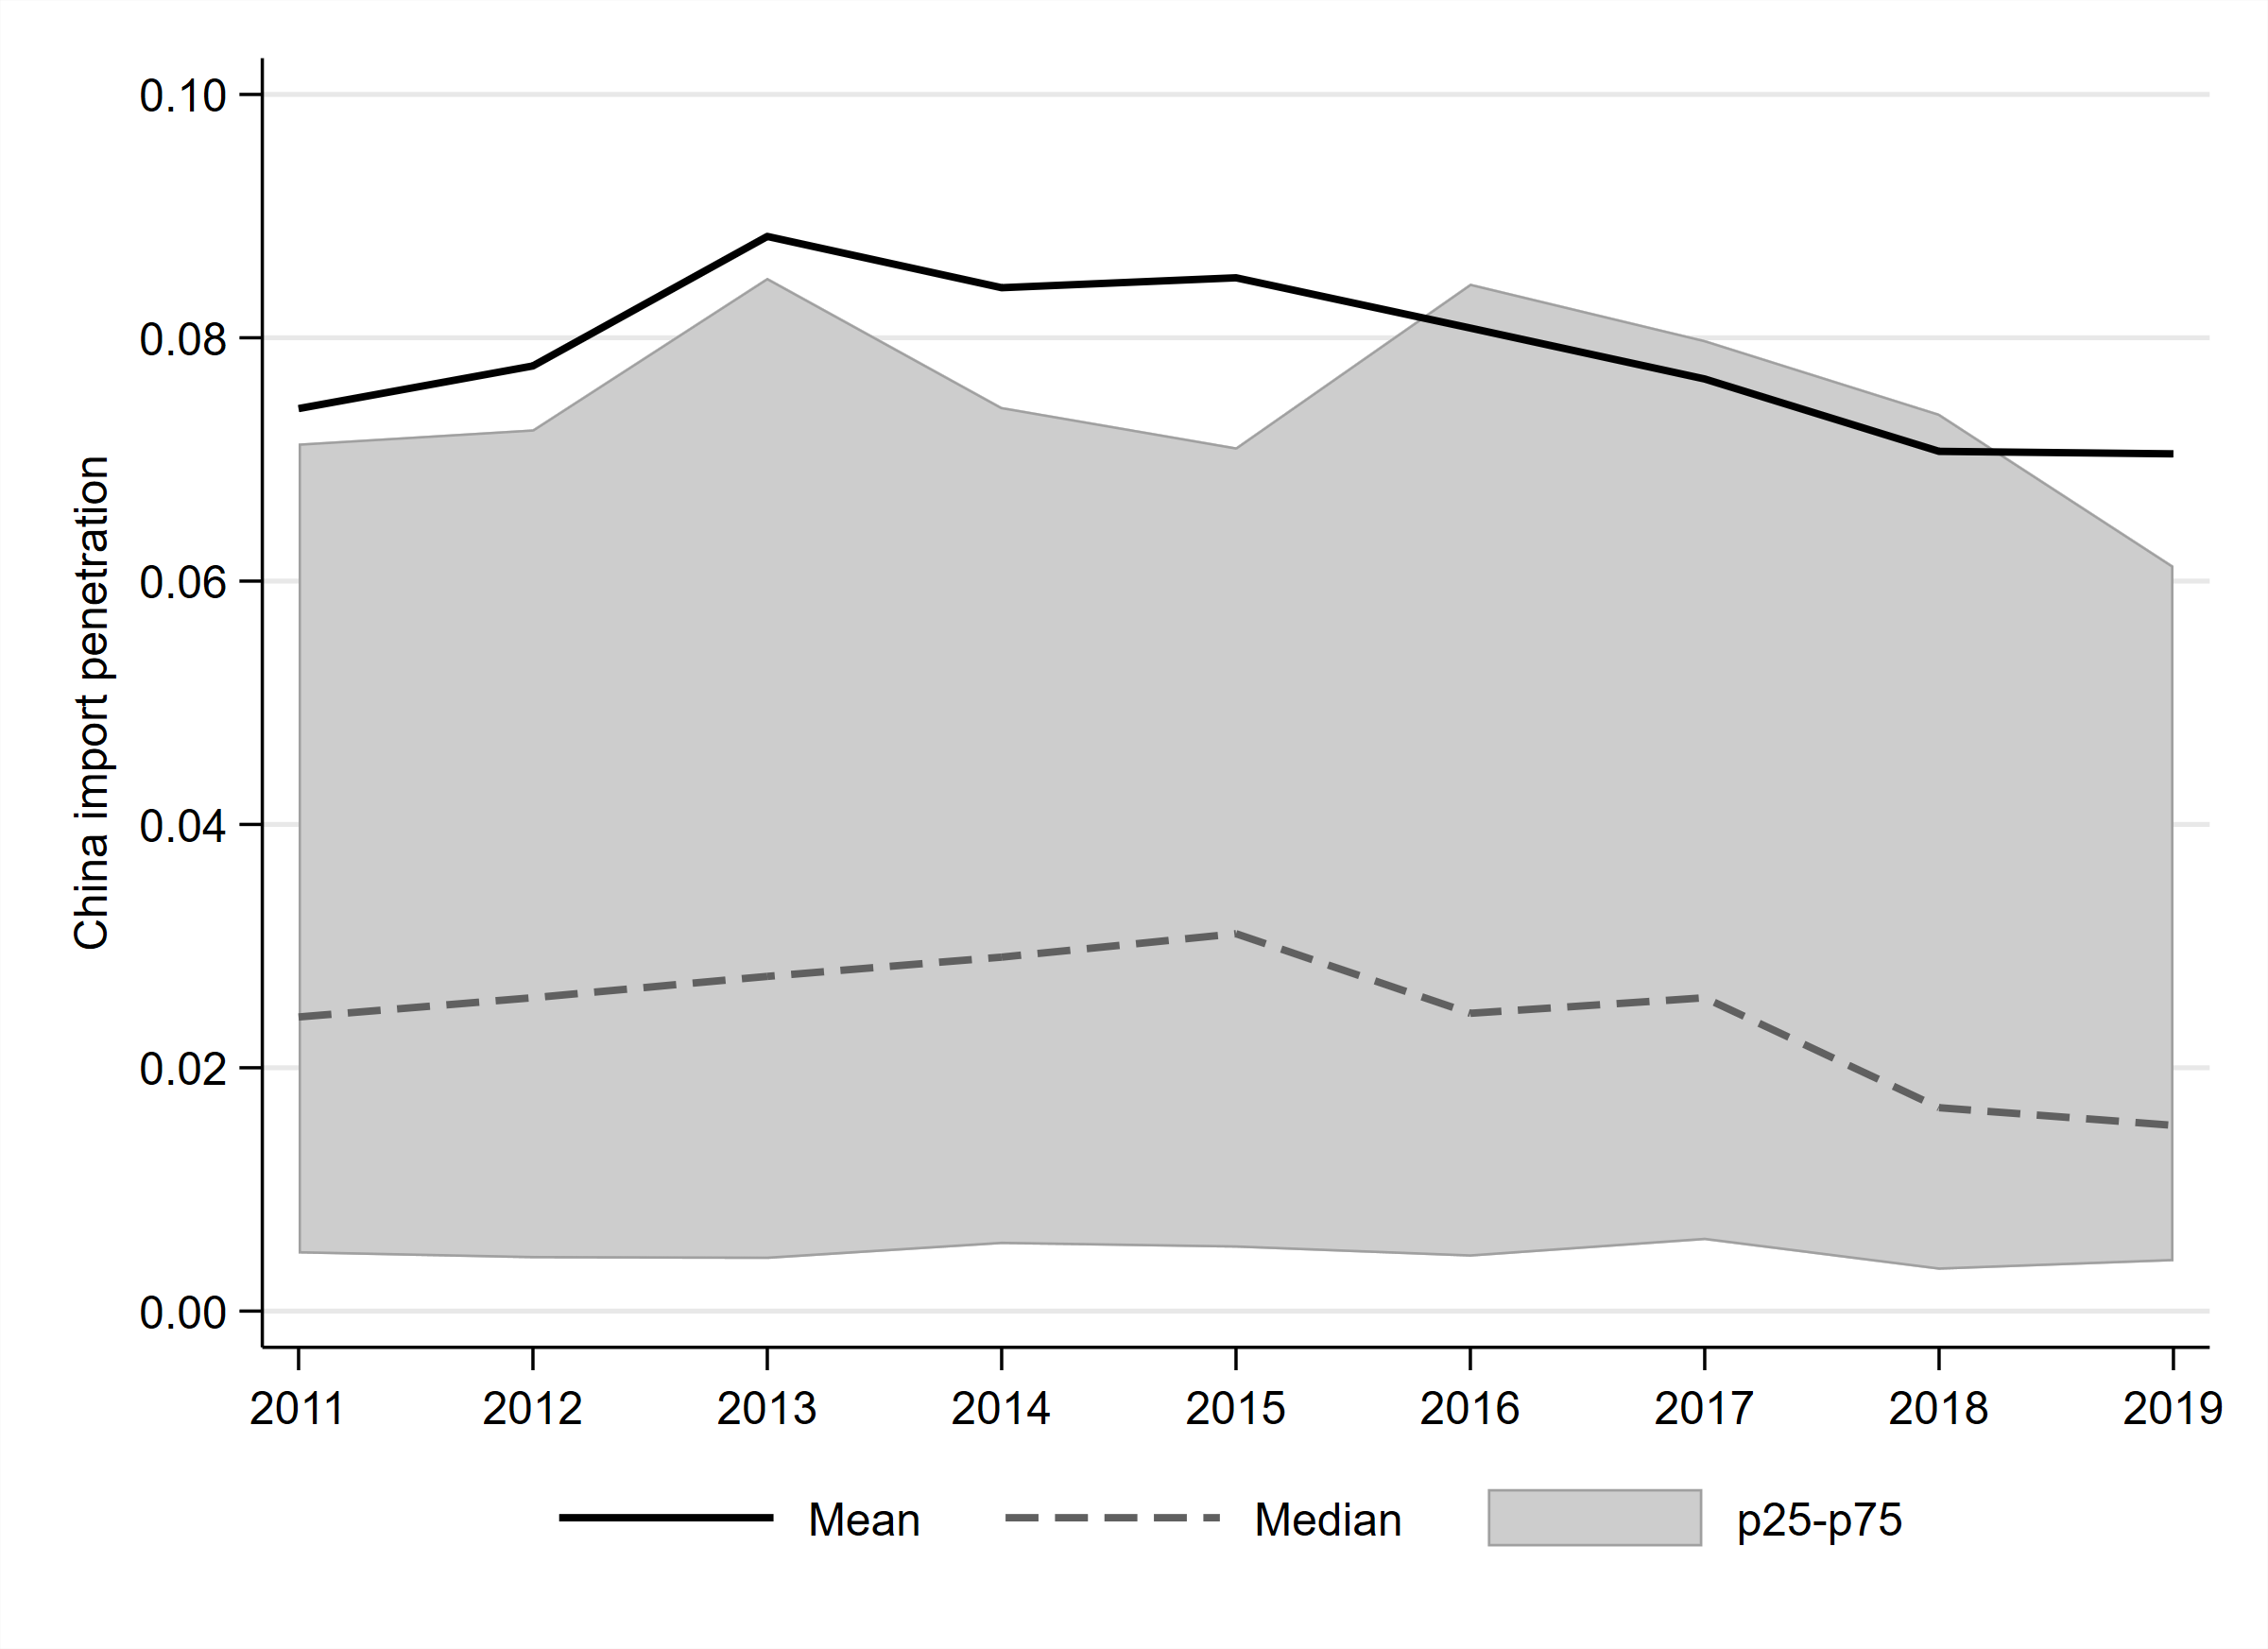
\includegraphics[width=0.64\textwidth]{fig_china_ip_context_trimmed.png}
    \caption{Chinese import penetration across Turkish manufacturing sectors}
    \label{fig:china_ip_context}
    \begin{minipage}{0.64\textwidth}
    \footnotesize
    \textit{Notes:} The figure reports the unweighted mean, median, and interquartile range of Chinese import penetration across ISIC4 manufacturing sectors in the 2011--2019 baseline trade-IV window.
    \end{minipage}
\end{figure}

\begin{figure}[H]
    \centering
    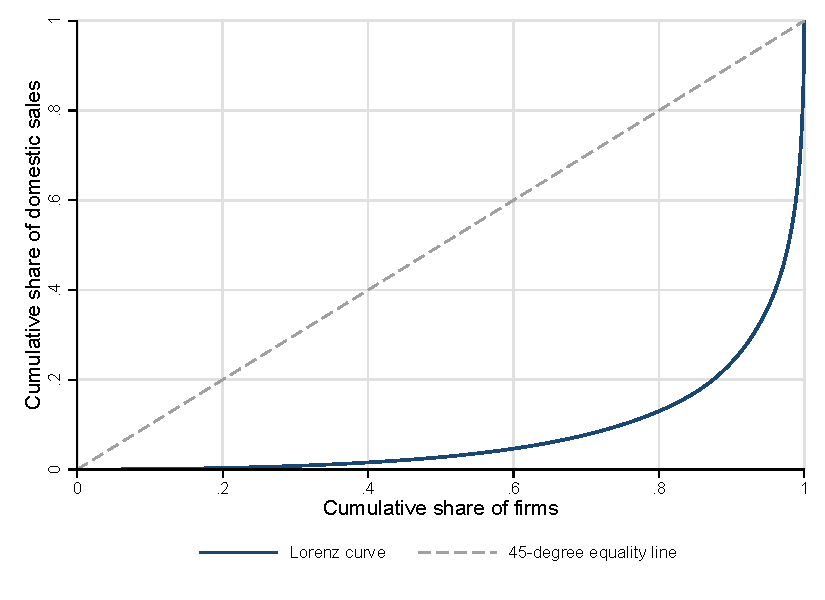
\includegraphics[width=0.64\textwidth]{lorenz_domestic_sales_2011.pdf}
    \caption{Lorenz curve of domestic sales among Turkish manufacturing firms}
    \label{fig:lorenz_domestic_sales}
    \begin{minipage}{0.86\textwidth}
    \footnotesize
    \textit{Notes:} Firms are ranked from smallest to largest by domestic sales share within ISIC4-year cells. Gini = 0.836; N = 6,112.
    The dashed line is the 45-degree equality benchmark. 
    The sample is restricted to firms with positive domestic sales in 2011.
    \end{minipage}
\end{figure}

Figure~\ref{fig:china_ip_context} summarizes the evolution of Chinese import penetration across Turkish manufacturing sectors. 
The average sector was more exposed than the median sector, indicating that Chinese penetration was concentrated in a subset of sectors rather than evenly distributed across manufacturing. 
This dispersion is useful for identification: the empirical strategy exploits differential sectoral exposure to Chinese import growth, rather than a single aggregate China shock affecting all Turkish manufacturers symmetrically.

A second feature of the setting is strong firm-size granularity. 
Figure~\ref{fig:lorenz_domestic_sales} plots the Lorenz curve of domestic sales among Turkish manufacturing firms in 2011. 
The curve lies far below the equality line, with a Gini coefficient of about 0.84. 
This indicates that a small upper tail of firms accounts for a disproportionate share of domestic sales. 
The figure makes an atomistic benchmark unattractive: large firms are economically important enough that their pricing and markup responses are likely to matter for aggregate and sectoral outcomes.

\begin{figure}[H]
    \centering
    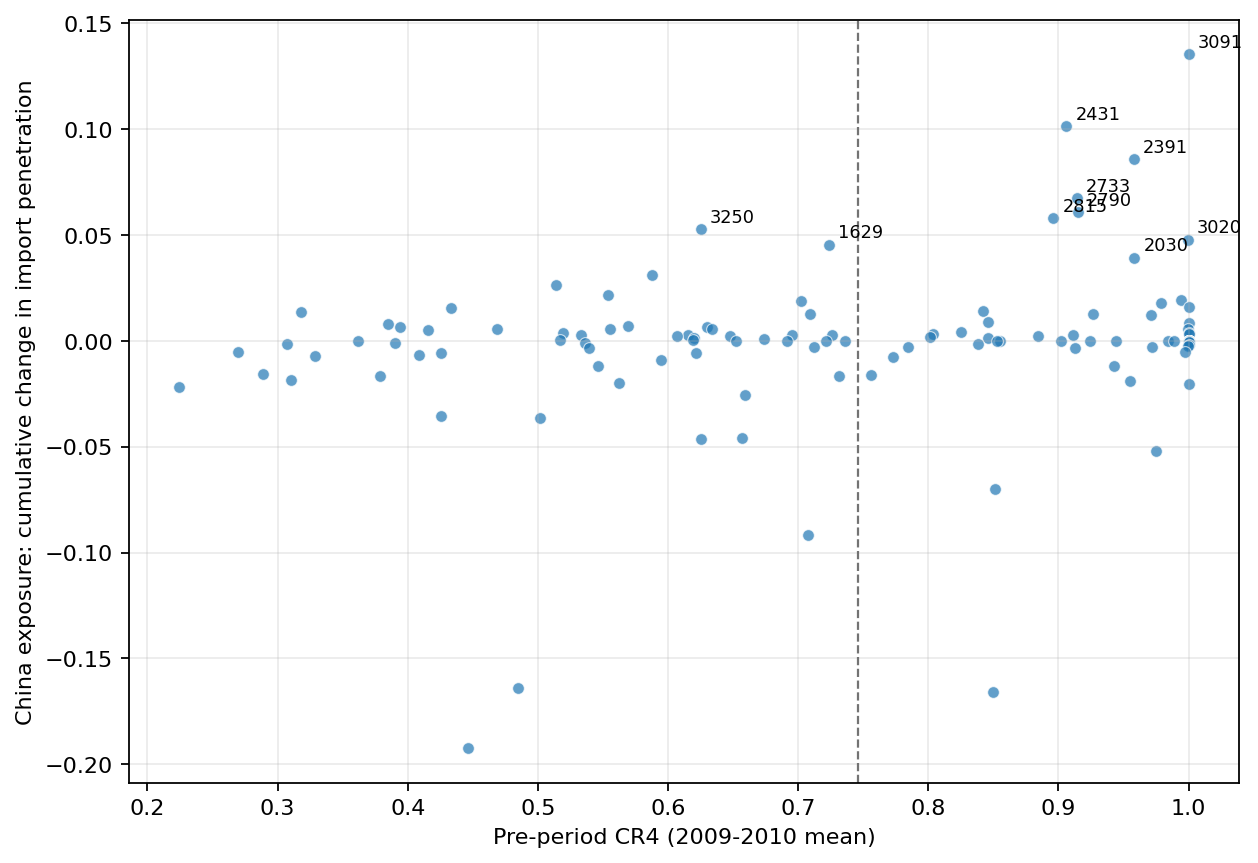
\includegraphics[width=0.72\textwidth]{scatter_CR4_pre_china_exposure.png}
    \caption{Chinese import exposure and pre-period sector concentration}
    \label{fig:china_exposure_pre_cr4}
    \begin{minipage}{0.86\textwidth}
    \footnotesize
    \textit{Notes:} Each point is an ISIC4 manufacturing sector. 
    The horizontal axis reports pre-period CR4, computed as the 2009--2010 mean domestic sales share of the four largest firms in the sector. 
    The vertical axis reports cumulative sector-level growth in Chinese import penetration over the available 2010s trade-exposure window.
    \end{minipage}
\end{figure}

\FloatBarrier

The exposure variation is also relevant for concentrated sectors. 
Figure~\ref{fig:china_exposure_pre_cr4} relates sector-level growth in Chinese import penetration to pre-period domestic concentration. 
Sectors with larger increases in Chinese exposure tend to have higher pre-period CR4, and the most exposed sectors are often located in the upper part of the pre-period concentration distribution. 
It shows that the China shock often arrived in industries where domestic market power was already empirically relevant, which is the environment in which foreign competition can discipline incumbent markups.

These facts motivate the Cournot oligopoly structure for Turkish manufacturing. The model below provides a tractable microfoundation for variable markups under finite-firm competition.

\section{Theoretical framework}
\label{sec:theory_model}

\subsection{Model}
This section presents the minimum theoretical backbone needed for the empirics. The model follows \textcite{atkesonPricingtoMarketTradeCosts2008, carvalhoProductionNetworksPrimer2019}, with domestic firms competing in quantities under nested CES demand and using imported intermediates in production. Detailed derivations of the nested CES system, the perceived elasticity formula, and the exit cutoff are in the Appendix \ref{app:theory_appendix}.

\textbf{Environment and demand}. The economy contains a continuum of sectors $j \in [0,1]$. In each sector, a finite set of domestic firms $i = 1,\ldots,N_j$ produces differentiated varieties and competes under Cournot. A representative household allocates expenditure across sectoral composites with elasticity $\eta > 1$, so sectoral absorption is
\[
D_j = \alpha_j \left(\frac{P_j}{P}\right)^{1-\eta} Y.
\]
Within each sector, expenditure is split between a domestic composite and a foreign composite with elasticity $\nu_j > 1$:
\[
Q_j = \left[(\Lambda_j^D)^{\frac{1}{\nu_j}} (Q_j^D)^{\frac{\nu_j-1}{\nu_j}} + (1-\Lambda_j^D)^{\frac{1}{\nu_j}} (Q_j^F)^{\frac{\nu_j-1}{\nu_j}}\right]^{\frac{\nu_j}{\nu_j-1}}.
\]
Within the domestic segment, varieties are aggregated with elasticity $\rho_j > 1$:
\[
Q_j^D = \left(\sum_{i=1}^{N_j} \xi_i^{\frac{1}{\rho_j}} q_{ij}^{\frac{\rho_j-1}{\rho_j}} \right)^{\frac{\rho_j}{\rho_j-1}}.
\]
I maintain $\rho_j > \nu_j > \eta$, so substitution is strongest across domestic varieties, weaker between domestic and foreign composites, and weakest across sectors. This ordering is what makes the output-competition effect stronger for firms with larger market shares and for more concentrated sectors.

\textbf{Production and the input channel}. Each firm produces according to
\[
q_{ij} = \varphi_{ij} L_{ij}^{\beta_j} M_{ij}^{1-\beta_j},
\qquad 0<\beta_j<1,
\]
which implies marginal cost
\[
\text{mc}_{ij} \propto \varphi_{ij}^{-1} w^{\beta_j} (P_j^M)^{1-\beta_j}.
\]
Log changes in intermediate-input prices propagate through the Turkish input-output network, so a reduced-form approximation to marginal-cost growth is
\begin{equation}
d \ln \text{mc}_{ij} \approx -d \ln \varphi_{ij} + \beta_j d \ln w + (1-\beta_j) \sum_k l_{jk} \omega_k^{CHN} d \ln P_k^{CHN}.
\label{eq:marginal_cost_io}
\end{equation}
This expression is the basis for the empirical input-supply channel: Chinese input shocks lower costs more in sectors with stronger upstream exposure.

\textbf{Oligopoly and markups}. Let $\tilde{s}_{ij}$ denote firm $i$'s share within the domestic segment and $s_{ij}$ its share in total sectoral expenditure. Under Cournot competition, the firm-specific perceived elasticity is
\[
\sigma_{ij}^C =
\left(
\frac{1-\tilde{s}_{ij}}{\rho_j}
+
\frac{\tilde{s}_{ij}-s_{ij}}{\nu_j}
+
\frac{s_{ij}}{\eta}
\right)^{-1}.
\]
The resulting optimal markup is $\mu_{ij} = \sigma_{ij}^C / (\sigma_{ij}^C-1)$, or, more usefully for interpretation,
\begin{equation}
\frac{1}{\mu_{ij}} =
\left(1-\frac{1}{\rho_j}\right)
-
\left[
\frac{1}{\Lambda_j^D}\left(\frac{1}{\nu_j}-\frac{1}{\rho_j}\right)
+
\left(\frac{1}{\eta}-\frac{1}{\nu_j}\right)
\right] s_{ij}.
\label{eq:firm_inverse_markup}
\end{equation}
Aggregating across firms with the market-share-weighted harmonic mean implies
\begin{equation}
\frac{1}{\mu_j} =
\left(1-\frac{1}{\rho_j}\right)
-
\left[
\frac{1}{\Lambda_j^D}\left(\frac{1}{\nu_j}-\frac{1}{\rho_j}\right)
+
\left(\frac{1}{\eta}-\frac{1}{\nu_j}\right)
\right] \text{HHI}_j.
\label{eq:sector_inverse_markup}
\end{equation}
Sectoral markups therefore rise with concentration, and the slope of that relationship depends on the domestic expenditure share $\Lambda_j^D$. Stronger foreign competition lowers $\Lambda_j^D$, steepens residual demand, and disciplines markups most in sectors where concentration is already high.

\textbf{Dynamic selection}. Following \textcite{golombekExitDynamicsStartup2018}, a firm that remains active in period $t$ receives current profits and retains the option value of future operation. If the firm stays active, its continuation value satisfies
\[
V(x_{ijt}) = \max \left\{0,\; \pi(x_{ijt}) + \beta \mathbb{E}[V(x_{ij,t+1}) \mid x_{ijt}] \right\}.
\]
Trade shocks affect both current profitability and continuation values, so observed firm-level outcomes among survivors are selected on latent state variables. This is why the empirical strategy later uses the selection-correction term for these unobserved state variables to check for non-random sample survival.

\subsection{Testable predictions and empirical mapping}

The static model gives a useful map for the empirical design. The firm-level inverse-markup condition in equation~\eqref{eq:firm_inverse_markup} shows that markups depend on the domestic expenditure share and on the firm's market-share state, while the sectoral aggregation in equation~\eqref{eq:sector_inverse_markup} shows that the same residual-demand force is amplified by concentration. A rise in Chinese import penetration reduces the domestic share of spending and makes residual demand more elastic for Turkish incumbents. The first prediction is therefore a disciplining effect of output-market import competition on incumbent markup growth. Because equations~\eqref{eq:firm_inverse_markup}--\eqref{eq:sector_inverse_markup} load this channel through firm shares and \(HHI_j\), the effect should be stronger where initial market power is larger, especially in more concentrated sectors and among firms with market-share states associated with pricing power.

The input channel is different. The marginal-cost expression in equation~\eqref{eq:marginal_cost_io} implies that cheaper or more abundant Chinese intermediates affect firms through production costs, with the strength of the channel depending on upstream input exposure. These cost changes can also reallocate sales across producers with different cost positions. The model therefore does not require the input channel to produce the same within-firm markup response as final-goods competition. I treat the input-supply shifter as a separate control in the baseline markup regressions and use the sectoral decomposition to study whether it operates mainly through reallocation.

The empirical specification translates these comparative statics into annual first differences. The main outcome is
\[
\Delta \log \hat\mu_{ijt}
=
\log \hat\mu_{ijt} - \log \hat\mu_{ij,t-1}.
\]
For small annual changes, this is the first-difference counterpart of equations~\eqref{eq:firm_inverse_markup} and~\eqref{eq:sector_inverse_markup}.\footnote{Appendix~\ref{app:bridge} gives the formal bridge from the static inverse-markup condition to the first-difference estimating equation.} A predicted increase in inverse markups corresponds to lower log-markup growth. The coefficient on instrumented import-penetration growth is therefore interpreted as a local reduced-form response of incumbent markup growth to an output-competition shock, conditional on fixed effects, lagged controls, and the input-supply shifter. Because the instrument is a shift-share design, the identifying variation is relative across sector-year cells and is most informative for the cells receiving the largest Rotemberg weights.

The grouped-IV quantile regressions and concentration interactions test whether discipline is concentrated where the model predicts residual-demand effects to be strongest. The sectoral decomposition separates within-firm adjustment from reallocation and observed sample turnover, so sector-level markup changes need not mirror the average incumbent response. Finally, because markup growth is observed only for continuing reporters, the selection diagnostic in Section~\ref{sec:selection} is interpreted as a reduced-form check for non-random survival.

\section{Data and measurement}
The empirical analysis combines Turkish firm accounts, sector-level trade exposure, and predetermined input-output linkages. The baseline estimates use 2011--2019, because that is the window in which the firm panel, trade variables, sectoral output, and shift-share instrument are consistently available.

\subsection{Data sources}
\textbf{Firm-level data.} The ORBIS/AMADEUS dataset contains harmonized balance-sheet, income-statement, and profit-and-loss information for firms. I use the Turkish manufacturing panel from 2009 to 2023 and map firms from NACE Rev.2 into 4-digit ISIC sectors using a concordance. The raw manufacturing panel contains 15,957 firms and 78,921 firm-year observations. The 2009--2010 observations provide lags and baseline exposure shares; post-2019 data appear in descriptive tables but not baseline estimates. Because the main dependent variable is markup growth, the estimation sample is necessarily smaller than the raw panel: a firm-year enters the baseline markup regressions only when current and lagged accounting variables are both observed and revenue, COGS, and capital are positive. After applying these restrictions, winsorizing extreme variables at the 1st and 99th percentiles, and adding lagged controls, the main firm-level specifications use about 31,000 firm-year observations.

The panel is unbalanced, and I do not impute intermittent reporting gaps. I define \emph{observed exit} as disappearance from ORBIS/AMADEUS from $t$ to $t+1$, $t+2$, $t+3$ to better capture firm turnover. This operational definition is useful for studying sample composition, but it is not equivalent to validated legal or economic firm death. Throughout, entry and exit refer to observed sample turnover.

A relevant institutional break occurs in 2016, when Turkey implemented a large one-time increase in the statutory minimum wage. The shock mattered especially for labor-intensive formal firms because it raised reported payroll costs and changed the incentives to remain in formal reporting systems. In ORBIS/AMADEUS, this appears as a coverage change or reporting attrition even when it is not validated firm death. To avoid attributing such differential post-2016 coverage changes to Chinese import competition, the baseline specifications control for pre-2016 sectoral labor intensity interacted with a post-2016 indicator. The control is predetermined with respect to the post-2016 episode and absorbs the fact that labor-intensive sectors were more exposed to this institutional shock.

\textbf{Trade data.} My main treatment variable is Chinese import penetration at the 4-digit ISIC sector-year level, defined as
\begin{equation}
    \begin{aligned}
    \text{China IP}_{jt} = \frac{\text{Import}_{jt}^{\text{CHN} \to \text{TR}}}{\text{Output}_{jt} + \text{Import}_{jt}^{\text{World} \to \text{TR}} - \text{Export}_{jt}^{\text{TR} \to \text{World}}} 
\end{aligned}
\end{equation}
where the denominator corresponds to domestic absorption. I construct the numerator from CEPII BACI HS96 bilateral trade data at the HS 6-digit level and map products to 4-digit ISIC sectors using the HS--ISIC concordance generated with the \texttt{concordance} package of \textcite{liaoConcordanceProductConcordance2020}. Appendix~\ref{app:hs_isic_concordance} documents the mapping procedure and the treatment of many-to-many product-industry links. Sectoral output and trade aggregates used in the denominator come from UNIDO ISDB4/INDSTAT4. The treatment in the regressions is the annual change in this import-penetration rate.

For the input-supply channel, I propagate the output-side shift-share shock through Turkish input-output linkages. The weights come from the 2003 Turkish input-output table in WIOD and are kept fixed over the sample period. Using pre-period weights is a deliberate trade-off: it cannot capture subsequent changes in sourcing networks, but it preserves a predetermined exposure matrix and avoids loading the upstream shifter with contemporaneous endogenous restructuring.

\textbf{Other data.} I use several TURKSTAT datasets to construct controls and deflators. The 3-digit Producer Price Index (PPI) is used to deflate nominal variables. Personnel-cost and value-added data from the Annual Industry and Service Statistics are used to construct pre-period sectoral labor intensity. Across the empirical sections, the firm-level outcome data are therefore combined with a sector-year treatment design and a smaller set of effective identifying cells.

Table \ref{tab:summary_statistics} reports summary statistics for firm-level and sector-level variables used in the baseline and mechanism analyses.

\begin{table}[!htbp]
\centering
\caption{Summary Statistics}
\label{tab:summary_statistics}
\small
\setlength{\tabcolsep}{5pt}

\begin{threeparttable}
\begin{tabular}{@{}lrrrrrr@{}}
\toprule
Variable & N & Mean & SD & P50 & Min & Max \\
\midrule

\multicolumn{7}{@{}l}{\textbf{Panel A: Firm-level}} \\
Markup adjustment      & 31339 & 0.002 & 0.141 & 0.001 & -3.873 & 4.184 \\
Observed exit          & 31339 & 0.083 & 0.276 & 0.000 & 0.000 & 1.000 \\
EBIT margin            & 31339 & 6.890 & 8.818 & 5.670 & -95.350 & 95.750 \\
Log size               & 31339 & 15.181 & 1.632 & 15.132 & 7.399 & 22.085 \\
Leverage               & 31339 & 0.229 & 0.205 & 0.193 & -0.053 & 2.024 \\
Liquidity ratio        & 31339 & 1.411 & 2.714 & 0.910 & 0.000 & 99.470 \\
Age                    & 31339 & 5.772 & 3.317 & 5.000 & 2.000 & 15.000 \\
Exporter status        & 31339 & 0.697 & 0.460 & 1.000 & 0.000 & 1.000 \\

\midrule
\multicolumn{7}{@{}l}{\textbf{Panel B: Sector-level}} \\
Chinese import penetration      & 609 & -0.000 & 0.027 & -0.000 & -0.224 & 0.213 \\
Final-goods competition         & 609 & -0.001 & 0.008 & -0.000 & -0.071 & 0.066 \\
Input-supply shocks             & 609 & -0.000 & 0.003 & -0.000 & -0.009 & 0.011 \\
Labor share (pre-period)        & 609 & 0.510 & 0.092 & 0.510 & 0.260 & 0.887 \\
Domestic concentration (HHI)    & 609 & 0.200 & 0.220 & 0.114 & 0.001 & 1.000 \\

\bottomrule
\end{tabular}

\begin{tablenotes}[flushleft]
\footnotesize
\item \textit{Notes:} Panel A reports firm-year variables in the baseline markup sample.
Observed exit is disappearance from ORBIS/AMADEUS between adjacent years.
Panel B reports sector-year variables for the 2011--2019 trade-IV design.
Chinese import penetration change, final-goods competition, and input-supply shocks are annual changes or shifters measured at the ISIC4-year level.
HHI is based on domestic sales among observed firms.
\end{tablenotes}

\end{threeparttable}
\end{table}

\subsection{Chinese import competition}
\label{sec:data_treatment}

Estimating the effect of changes in Chinese import penetration on firm outcomes by OLS is problematic for at least three reasons. First, Turkish sectoral demand or productivity shocks may affect both imports from China and domestic firm outcomes. Second, persistent sectoral characteristics may jointly shape exposure to Chinese competition and firm performance. Third, the treatment varies at the sector-year level while the main outcomes are observed at the firm-year level, so naive firm-level regressions risk overstating the amount of independent identifying variation.

I implement a shift-share IV following \textcite{autorTradeAdjustmentWorkerLevel2014}, combining Chinese export growth to other high-income markets with predetermined 2009 Turkish exposure shares. This isolates China-driven variation from contemporaneous Turkish shocks.

The instrument combines Chinese export-share growth $g_{jt}$ (change in China's share in high-income markets) with baseline Turkish exposure $s_{j,\text{CHN}}^{2009}$:
\[
Z_{jt}^{\text{Output}} = s_{j,\text{CHN}}^{2009} \times g_{jt}.
\]
The input control propagates output shocks through input-output linkages: $Z_{jt}^{\text{Input}} = \sum_k w_{jk}^{2003} Z_{kt}^{\text{Output}}$, where $w_{jk}^{2003}$ is the share of sector $k$ in sector $j$'s intermediate inputs.

The treatment cell is sector-year (611 cells across 95 sectors in the baseline IV sample). Identification assumes the shift is orthogonal to residual sectoral shocks after absorbing fixed effects and controls; this is most credible for cells with strong supply-side China exposure. Lead-placebo and Rotemberg-weight diagnostics confirm the estimate is local to influential exposed cells, not universal across all Turkish manufacturing.


\subsection{Markup estimation and other variables}

\textbf{Markups.} I estimate markups using the production approach pioneered by \textcite{hallRelationPriceMarginal1988} and developed by \textcite{deloeckerMarkupsFirmLevelExport2012,deloeckerRiseMarketPower2020}. In the baseline implementation, I estimate a Cobb-Douglas revenue production function within ISIC4 sectors, use COGS as the flexible input, and recover the output elasticity of COGS from that production function. The markup estimator is
\[
\mu_{it} = \theta_{ivt} \frac{P_{it}Q_{it}}{P_{vit}V_{it}},
\]
where $\theta_{ivt}$ is the output elasticity of the flexible input, $P_{it}Q_{it}$ is firm revenue, and $P_{vit}V_{it}$ is expenditure on input $v$. COGS is the most consistently observed short-run variable input in ORBIS/AMADEUS and is therefore the baseline flexible input. Under the Cobb--Douglas baseline, the COGS elasticity is constant within sector, so changes in the measured markup are driven mechanically by changes in the revenue-to-COGS ratio. The cleanest interpretation is therefore not that I observe physical price-cost margins directly; it is that I study annual changes in a production-adjusted revenue-to-COGS markup proxy. Appendix~\ref{app:markup_estimation} reports the implementation details, a translog sensitivity check and robustness exercises from \textcite{kirovMeasuringMarkupsRevenue2026}.

Because accounting-based markup levels are sensitive to production-function assumptions, reporting quality, and the choice of flexible input, I focus on within-firm changes rather than levels \parencite{deridderHitchhikersGuideMarkup2026}. This choice removes time-invariant level differences but does not solve all measurement concerns. If Chinese exposure raises COGS through input costs or labor-cost pass-through, the markup proxy can fall even without a pure residual-demand response. The empirical design therefore controls for the input-supply shifter and labor-intensity exposure, but the resulting coefficient should still be read as evidence on markup-proxy dynamics rather than as a direct price-cost-margin estimate. The main dependent variable is
\[
\Delta \log \hat{\mu}_{it} \equiv \log \hat{\mu}_{it} - \log \hat{\mu}_{i,t-1}
\]
This choice is meant to limit the influence of time-invariant reporting differences and level mismeasurement.

\textbf{Labor Intensity.} Labor intensity is constructed as the ratio of personnel costs to value added factor cost, averaged over 2009--2015 at the 4-digit sector level. This time-invariant measure captures differences in production technology across industries. Following the institutional discussion above, the interaction of labor intensity with a post-2016 dummy captures differential exposure to the minimum-wage episode and the associated risk of formal-firm reporting attrition in ORBIS/AMADEUS.

\textbf{Sectoral Markup.} Following \textcite{bursteinBottomUpMarkupFluctuations2025}, sectoral markup is defined as the market-share-weighted harmonic mean of firm markups:
\[
\mu_{jt} = \left( \sum_{i \in j} s_{ijt} \mu_{it}^{-1} \right)^{-1}
\]
where $s_{ijt} = D_{it}/\sum_{i' \in j} D_{i't}$ is firm market share, which is firm domestic sales deflated by industry PPI. The harmonic mean is appropriate because it gives more weight to low-markup firms, which are more likely to be affected by import competition and selection. The change in sectoral markup is then defined as the first difference of the log of the sectoral markup.


\section{Empirical strategy}
\label{sec:empirical_strategy}
The empirical strategy has four components. Section 5.1 states the baseline shift-share IV specification and the identifying assumptions, with particular emphasis on the local sector-year cells that identify the estimate. Section 5.2 asks whether selective survival in the observed panel materially changes the within-incumbent estimate on an observed profitability proxy. Sections 5.3 and 5.4 then connect the mean result to sectoral aggregation and distributional heterogeneity through a decomposition and grouped IV quantile regressions.

\subsection{Identification strategy and baseline IV regression}
\label{sec:empirical_strategy_iv}

My baseline IV specification estimates the effect of changes in Chinese import penetration on firm-level markup adjustments, controlling for the input-supply channel and other covariates. The regression is specified as follows:
\begin{equation}
\begin{aligned}
Y_{ijt} &= \beta_O \Delta IP_{jt} + \beta_I Z_{jt}^{\text{Input}} + \gamma_1 \text{LaborShare}_{jt_0} \times \text{Post2016}_t \\
&\quad + \gamma_2 \text{LaborShare}_{jt_0} + X'_{ijt-1} \gamma + \tau_t + \delta_j + \varepsilon_{ijt}
\end{aligned}
\end{equation}

where $Y_{ijt}$ is the outcome of interest (observed exit probability at $t+1$ or markup adjustments), $\Delta IP_{jt}$ is the change in Chinese import penetration, $Z_{jt}^{\text{Input}}$ is the control variable for the input-supply channel, $\text{LaborShare}_{jt_0}$ is the pre-2016 averaged labor intensity, $X_{ijt-1}$ are lagged firm-level controls, and $\tau_t$ and $\delta_j$ are year and sector fixed effects. The coefficient of interest is $\beta_O$, which measures the effect of output-market import competition after controlling for upstream input shocks and observables.

Identification comes from the output-side shift-share IV $Z_{jt}^{\text{Output}}$ for $\Delta IP_{jt}$, while $Z_{jt}^{\text{Input}}$ remains included as a control. Two clarifications define the estimand. First, the treatment cell is the sector-year and the baseline exposure share is fixed in 2009, so the firm-level regression does not create additional independent shocks beyond those sector-year cells. Second, the coefficient is a local effect for the sector-year cells that receive the most identifying weight. Figure~\ref{fig:rotemberg_sector_size} shows that the largest Rotemberg-weight sectors are economically small but highly exposed to Chinese imports in 2009. The appendix exclusion exercise shows that once the most influential Rotemberg-weight sectors are removed, the first stage weakens sharply and the second-stage estimate becomes unstable in both sign and magnitude. I therefore treat the baseline IV as evidence that Chinese import competition disciplines markups in influential exposed sectors.

\begin{figure}[htbp]
    \centering
    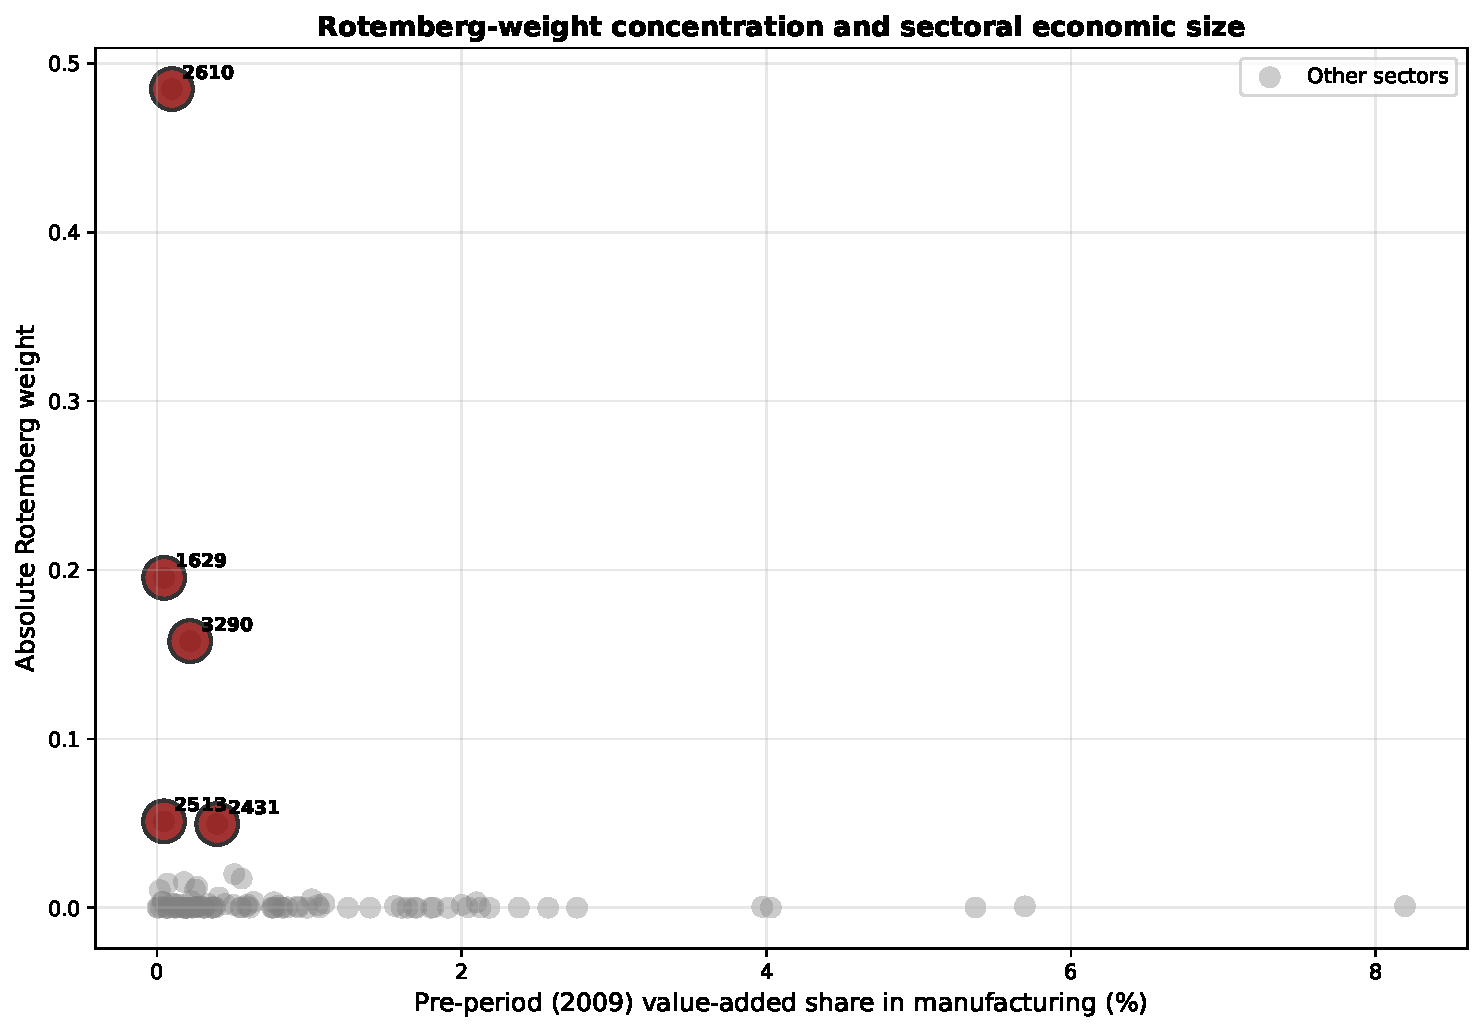
\includegraphics[width=0.82\textwidth]{fig_rotemberg_sector_size.pdf}
    \caption{Top Rotemberg-weight sectors and pre-period economic size}
    \label{fig:rotemberg_sector_size}
\end{figure}

The control for pre-2016 labor share interacted with the post-2016 dummy captures differential exposure to the minimum-wage episode, which may have affected the formal-firm coverage \parencite{akcigitFactsBusinessDynamism2020}. Because firms with similar exposure structures may have correlated residuals, inference is clustered at the ISIC4 level and complemented, where available, with wild-cluster bootstrap p-values in the robustness section.

Lead-placebo tests verify exclusion restriction: future China shocks should not predict current outcomes. Significant placebo coefficients would indicate pre-trends or omitted confounders.

Formally, for horizon $k \in \{1,2,3\}$, I estimate:
\begin{equation}
\begin{aligned}
Y_{ijt} &= \beta^{k}_O Z^{\text{Output}}_{j,t+k} + \beta_I0 Z_{jt}^{\text{Input}} + \beta_{I1} Z_{j,t-1}^{\text{Input}} + \gamma_1 \text{LaborShare}_{jt_0} \times \text{Post2016}_t \\
&\quad + \gamma_2 \text{LaborShare}_{jt_0} + X'_{ijt-1} \gamma + \tau_t + \delta_j + \varepsilon_{ijt}
\end{aligned}
\end{equation}

Under identifying assumptions, placebo coefficients should be statistically indistinguishable from zero, supporting instrument validity.

\begin{figure}[htbp]
    \centering
    \begin{tikzpicture}
    \begin{axis}[
        width=0.92\textwidth,
        height=7.2cm,
        xmin=-1.05, xmax=0.80,
        ymin=0.5, ymax=3.5,
        axis x line=bottom,
        axis y line=left,
        xlabel={Coefficient on future shock},
        ylabel={Future horizon},
        ytick={1,2,3},
        yticklabels={t+3, t+2, t+1},
        xtick={-1.0,-0.5,0,0.5,0.8},
        xmajorgrids=true,
        ymajorgrids=false,
        grid style={dashed, draw=gray!20},
        major grid style={line width=0.3pt},
        tick align=outside,
        tick style={black},
        axis line style={black},
        clip=false,
    ]

    \addplot[dashed, gray!70, thick] coordinates {(0,0.5) (0,3.5)};

    \addplot[
        only marks,
        mark=*,
        mark size=2.8pt,
        blue!70!black
    ] coordinates {(0.48,3)};
    \addplot[
        blue!70!black,
        thick,
        error bars/.cd,
        x dir=both,
        x explicit
    ] coordinates {(0.48,3) +- (0.50,0)};

    \addplot[
        only marks,
        mark=*,
        mark size=2.8pt,
        magenta!75!black
    ] coordinates {(-0.08,2)};
    \addplot[
        magenta!75!black,
        thick,
        error bars/.cd,
        x dir=both,
        x explicit
    ] coordinates {(-0.08,2) +- (0.90,0)};

    \addplot[
        only marks,
        mark=*,
        mark size=2.8pt,
        teal!70!black
    ] coordinates {(-0.23,1)};
    \addplot[
        teal!70!black,
        thick,
        error bars/.cd,
        x dir=both,
        x explicit
    ] coordinates {(-0.23,1) +- (0.38,0)};

    \end{axis}
    \end{tikzpicture}
    \caption{Placebo: future shocks predicting current markup changes}
    \label{fig:my_plot}
\end{figure}

The results in Figure \ref{fig:my_plot} support the timing restriction behind the design. Across the one to three-year horizons, the estimated placebo coefficients are small, not systematically signed, and statistically insignificant, suggesting no evidence that future China shocks predict current markup changes. This check does not prove the exclusion restriction, but it reduces concern that the baseline estimate is driven by simple pre-trends or reverse causality.

\subsection{Selection diagnostic}
\label{sec:selection}

A key concern in the baseline regression is endogenous sample selection. Firm-level markup adjustments are observed only for firms that remain in the panel and continue reporting. In ORBIS/AMADEUS, disappearance may reflect true economic exit, reporting gaps, or coverage changes. The empirical problem is the same in each case: if Chinese import competition affects observed survival and that margin is correlated with unobserved determinants of markup adjustment, then the baseline IV estimates mix a within-firm response with compositional change in the observed sample.

To address this issue, I adopt a semiparametric control-function diagnostic inspired by the selection approach in \textcite{backusWhyProductivityCorrelated2020,pavcnikTradeLiberalizationExit2002}. The objective is to test whether a flexible proxy for latent firm state materially changes the markup estimate. If observed survival depends on latent firm state and that state also affects markup adjustment, then the regression error among observed firms is not mean-independent of trade exposure.

I proxy the latent state with lagged EBIT margin, denoted $s_{i,t-1}$. This variable is observable, persistent, predictive of observed exit, and informative about subsequent markup adjustment, so it provides a practical control-function index for selection. Let the second-stage error decompose as $\varepsilon_{i(j)t} = \lambda_{jt} + \eta_{it}$, where $\lambda_{jt}$ captures sector-year shocks and $\eta_{it}$ is an idiosyncratic component. Among surviving firms, I model the selection-induced component as a flexible function of the lagged state proxy,
\[
\mathbb{E}[\eta_{it} \mid s_{it-1}] = g(s_{it-1}),
\]
and approximate $g(\cdot)$ with a third-order polynomial in $s_{it-1}$. The cubic is flexible enough to capture nonlinear selection on profitability without overfitting a relatively small support of the state proxy. The diagnostic second-stage regression therefore includes this control function:
\begin{equation}
\begin{aligned}
\Delta \ln \mu_{i(j)t} &= \beta_O \widehat{\Delta IP_{jt}} + \beta_I Z_{jt}^{\text{Input}} + \gamma_1 \text{LaborShare}_{jt_0} \times \text{Post2016}_t \\
&\quad + \gamma_2 \text{LaborShare}_{jt_0} + X'_{ijt-1} \gamma + \tau_t + \delta_j + g(s_{it-1}) + \epsilon_{i(j)t}
\end{aligned}
\end{equation}

Conditional on the flexible control function $g(s_{it-1})$, the remaining variation in the instrumented import penetration shock gives a reduced-form check of whether the baseline estimate is sensitive to selection on the observed state proxy. Thus, $\beta_O$ should still be interpreted as a within-incumbent effect among observed survivors. The control function shows whether the estimate is stable after conditioning on lagged profitability; it does not prove that all selection bias has been removed.

\begin{table}[!htb]\centering
    \def\sym#1{\ifmmode^{#1}\else\(^{#1}\)\fi}
    \caption{Validation of Lagged EBIT Margin as State Proxy}
    \label{tab:ebit_validation}
    \footnotesize
    \setlength{\tabcolsep}{3pt}
    \renewcommand{\arraystretch}{0.95}
    \begin{threeparttable}
    \begin{fittabular}{L{0.28\textwidth}*{5}{c}}
    \toprule
    & \theadstack{(1)\\Persistence} & \theadstack{(2)\\Observed Exit\\(linear)} & \theadstack{(3)\\Observed Exit\\(quadratic)} & \theadstack{(4)\\Markup\\Adjustments} & \theadstack{(5)\\Markov\\Test} \\
    \midrule
    $\text{EBIT Margin}_{t-1}$ & 0.0437\sym{***} & -0.000453\sym{**} & -0.000524\sym{**} & -0.00876\sym{***} & -0.000977\sym{***} \\
    & (0.0164) & (0.000229) & (0.000237) & (0.000528) & (0.000306) \\
    \addlinespace[0.15em]
    $\text{EBIT Margin}_{t-1}^2$ & & & -0.0000133\sym{***} & & \\
    & & & (0.00000482) & & \\
    \addlinespace[0.15em]
    $\text{EBIT Margin}_{t-2}$ & & & & & 0.0000519 \\
    & & & & & (0.000287) \\
    \midrule
    Observations & 41,113 & 41,150 & 41,150 & 41,150 & 29,326 \\
    $R^2$ & 0.649 & 0.341 & 0.341 & 0.356 & 0.367 \\
    \bottomrule
    \end{fittabular}
    \begin{tablenotes}[flushleft]
    \scriptsize
    \item Notes: Standard errors clustered at firm level in parentheses. All specifications include firm, sector (ISIC4), and year fixed effects. Controls: leverage, liquidity ratio, log firm size, age, export status, and labor share $\times$ Post-2016 indicator; sample 2011--2019.
    \item Column (1) tests persistence; columns (2)--(3) test predictive power for observed exit; column (4) tests markup adjustments among survivors; column (5) reports the Markov test (lagged EBIT margin at $t-2$, p-value 0.857).
    \item \sym{*} \(p<0.10\), \sym{**} \(p<0.05\), \sym{***} \(p<0.01\).
    \end{tablenotes}
    \end{threeparttable}
    \renewcommand{\arraystretch}{1}
\end{table}

Table \ref{tab:ebit_validation} examines whether lagged EBIT margin is informative enough to serve as this state proxy. The evidence supports its use for a diagnostic. First, lagged EBIT margin is persistent over time, consistent with a slowly evolving firm state. Second, it predicts observed exit. Third, it is associated with future markup adjustments among survivors, indicating that it captures economically relevant heterogeneity in firms' dynamic responses. Finally, the Markov restriction is supported by the data: once lagged EBIT margin at $t-1$ is included, the additional lag at $t-2$ is not significant. This does not prove that EBIT margin is a sufficient statistic for selection; it shows that the baseline result is not sensitive to a practical reduced-form profitability proxy. 

\subsection{Decomposition of sectoral markup changes}
\label{sec:decomposition}

Firm-level regressions identify whether Chinese import penetration disciplines incumbents' pricing behavior, but they do not by themselves show how these responses aggregate to the sector level. This matters because sectoral markups may move differently from firm-level markups when import shocks also reallocate market shares across incumbents or change which firms are observed in adjacent years. To connect micro responses to sector-wide outcomes, I therefore decompose annual changes in sectoral markups into within-firm, reallocation, observed entry, and observed exit components. This decomposition is suited to environments with variable markups, where sectoral markup movements depend jointly on firm-specific markup adjustment and changes in market shares. 

Let $S_t$ denote the set of firms observed in sector $j$ at time $t$, $C = S_{t-1} \cap S_t$ the set of continuing firms, $E = S_t \setminus S_{t-1}$ observed entrants, and $X = S_{t-1} \setminus S_t$ observed exiters. Adapted from \textcite{melitzDynamicOlleyPakesProductivity2015}, the change in sectoral inverse markup can then be written as:
\[\Delta \mu_{jt}^{-1}
=
\underbrace{\sum_{i \in C} \bar{s}_{ij}\,\Delta \mu_{ij}^{-1}}_{\text{Within (continuers)}}
+
\underbrace{\sum_{i \in C} \Delta s_{ij}\,\bar{\mu}_{ij}^{-1}}_{\text{Between (continuers)}}
+
\underbrace{\sum_{i \in E} s_{ijt}\,\mu_{ijt}^{-1}}_{\text{Observed entry}} - \underbrace{\sum_{i \in X} s_{ij,t-1}\,\mu_{ij,t-1}^{-1}}_{\text{Observed exit}}\]
where $\bar{s}_{ij} = \frac{1}{2}(s_{ijt} + s_{ijt-1})$ and $\bar{\mu}_{ij}^{-1} = \frac{1}{2}(\mu_{it}^{-1} + \mu_{it-1}^{-1})$ are the average market share and inverse markup for firm $i$ over the two periods. This decomposition allows me to isolate the contributions of different mechanisms to sectoral markup changes.

The within term captures incumbent adjustment; the reallocation term captures market-share shifts across continuing firms; entry and exit terms capture composition changes. Because the decomposition is written in inverse markups, a positive component corresponds to a decline in sectoral markups, that is, a pro-competitive effect, while a negative component corresponds to an increase in sectoral markups, that is, an anti-competitive effect.

For each component $m \in \{ \text{within-firm, reallocation, observed entry, observed exit} \}$, I regress it on import penetration and controls, which shows how the import-competition effect can operate through distinct channels. 
\begin{equation}
\begin{aligned}
    Y^m_{jt} &= \beta_O^m \widehat{\Delta IP}_{jt} + \beta_I^m Z_{jt}^{\text{Input}} + \Gamma' W_{jt} + \delta_j + \tau_t + \epsilon_{jt}^m
\end{aligned}
\end{equation}
where $Y^m_{jt}$ is the sector-level outcome corresponding to component $m$, $\widehat{\Delta IP_{jt}}$ is the change in Chinese import penetration instrumented by the output-competition shock, $Z_{jt}^{\text{Input}}$ is the control for input supply channel, $W_{jt}$ are sector-level controls, and $\delta_j$ and $\tau_t$ are sector and year fixed effects. The coefficient $\beta_O^m$ captures the effect of import competition on the specific channel $m$.

Sectoral aggregate effects need not mirror firm-level responses when reallocation or composition effects may offset within-firm discipline. Separating these margins clarifies the mechanisms behind sectoral markup changes. 

\subsection{Distributional effects and concentration heterogeneity}
\label{sec:distributional}

To move beyond average effects, I examine whether import competition shifts different parts of the within-sector-year distribution of firm-level markup adjustments. This is important because mean IV estimates may mask whether trade discipline is concentrated in the upper tail of markup-growth realizations, where firms are attempting the largest positive adjustments. I therefore complement the baseline specification with a grouped IV quantile approach \textcite{chetverikovIVQuantileRegression2016} adapted to the setting in which the endogenous treatment varies at the sector-year level.

I define $\rho_{jt}^{(k)}$ as the $k$-th decile of the distribution of the within-sector-year distribution of firm-level markup adjustments among survivors. For each decile $k$, the regression is specified as:
\begin{equation}
\begin{aligned}
\rho_{jt}^{(k)} &= \beta_O^{(k)} \widehat{\Delta IP_{jt}} + \beta_I^{(k)} Z_{jt}^{\text{Input}} + \gamma_1^{(k)} \text{LaborShare}_{jt_0} \times \text{Post2016}_t \\
&\quad + \gamma_2^{(k)} \text{LaborShare}_{jt_0} + X'_{jt-1} \gamma^{(k)} + \tau_t^{(k)} + \delta_j^{(k)} + \nu_{jt}^{(k)}
\end{aligned}
\end{equation}

The grouped formulation is preferable to a standard firm-level IV quantile regression because the treatment is common within sector-year cells. Pooling firms directly would require rank-similarity assumptions across sectors that are difficult to justify in the presence of sector-level unobservables. By using sector-year quantiles as the dependent variable, the specification isolates how import competition shifts group-level outcome quantiles.

Identification relies on the same shift-share design as in the baseline analysis. Sectoral changes in Chinese import penetration are instrumented using exogenous growth in Chinese exports to high-income destinations interacted with predetermined Turkish exposure shares, while controlling for the input supply channel. Conditional on fixed effects and controls, $\widehat{\Delta IP_{jt}}$ is therefore interpreted as exogenous variation in output-market competitive pressure. 

Because sample quantiles are mechanically sensitive to the number of firms in each sector-year cell, particularly in smaller sectors, I correct for order-statistic bias (Neyman and Scott, 1948) by augmenting the specification with a flexible control function of the number of firm observations $n_{jt}$:
\begin{equation}
\begin{aligned}
\rho_{jt}^{(k)} &= \beta_O^{(k)} \widehat{\Delta IP_{jt}} + \beta_I^{(k)} Z_{jt}^{\text{Input}} + \gamma_1^{(k)} \text{LaborShare}_{jt_0} \times \text{Post2016}_t \\
&\quad + \gamma_2^{(k)} \text{LaborShare}_{jt_0} + X'_{jt-1} \gamma^{(k)} + \tau_t^{(k)} + \delta_j^{(k)} + g^{(k)}(n_{jt}) + \nu_{jt}^{(k)}
\end{aligned}
\end{equation}
where $g^{(k)}(\cdot)$ is approximated with a third-order polynomial in $n_{jt}$. This follows the correction proposed in \textcite{backusWhyProductivityCorrelated2020}, where order statistics can be spuriously correlated with group size when the number of firms is small relative to the number of quantiles. The appendix Monte Carlo shows why this correction matters: without a cell-size control, a null design in which sector-year cell size is correlated with the instrument over-rejects sharply at upper quantiles; the cubic control and the targeted spline-bootstrap correction bring the false rejection rate much closer to nominal size.

I then study heterogeneity in the pro-competitive effect by interacting predicted import penetration with lagged domestic concentration measures (CR10/CR4):
\begin{equation}
\begin{aligned}
\rho_{jt}^{(k)} &= \beta_{O1}^{(k)} \widehat{\Delta IP_{jt}} + \beta_{O2}^{(k)} \widehat{\Delta IP_{jt}} \times \text{Concentration}_{jt-1} + \beta_I^{(k)} Z_{jt}^{\text{Input}}  + \gamma_2^{(k)} \text{LaborShare}_{jt_0} \\
&\quad + \gamma_1^{(k)} \text{LaborShare}_{jt_0} \times \text{Post2016}_t + X'_{jt-1} \gamma^{(k)} + \tau_t^{(k)} + \delta_j^{(k)} + g^{(k)}(n_{jt}) + \nu_{jt}^{(k)}
\end{aligned}
\end{equation}

This specification tests whether import competition exerts stronger disciplinary effects in sectors where domestic market power is initially more concentrated. The same logic is extended to additional mechanism tests using interactions with baseline sectoral characteristics, such as initial markup levels, size, or revenue growth.

\section{Results}

\subsection{First stage and identification diagnostics}
\label{sec:first_stage_diagnostics}

I first assess the relevance of the output-side instrument and the separation between the output-competition and input-supply channels. Table~\ref{tab:firststage} reports first-stage regressions of sectoral Chinese import penetration on the output-side instrument \(Z^{\text{Output}}_{jt}\), controlling for the input-supply shifter \(Z^{\text{Input}}_{jt}\), sector fixed effects, and year fixed effects. The parsimonious specification includes only these design controls, while the baseline specification also includes the lagged firm-level controls used in the second stage. Because treatment varies at the sector-year level, the firm-year count overstates the amount of independent identifying variation; the baseline IV sample contains 611 sector-year cells across 95 sectors.

The output-side instrument is strongly predictive of realized import-penetration changes. In both columns, the coefficient on \(Z^{\text{Output}}_{jt}\) is 0.892, with a standard error of 0.179. The corresponding cluster-robust first-stage \(F\)-statistic is about 24.8. Thus, Chinese export growth to other high-income destinations is a strong predictor of import competition in Turkish manufacturing sectors. This relevance result should nevertheless be interpreted together with the Rotemberg diagnostics below, which show that identifying weight is concentrated in a subset of highly exposed sectors.

The input-supply shifter does not explain the first stage. Its coefficient is small and statistically insignificant in both specifications. This matters for interpretation: conditional on sector and year fixed effects, realized import penetration is predicted by the output-side China shock rather than by upstream input-supply exposure. The modest correlation between \(Z^{\text{Output}}_{jt}\) and \(Z^{\text{Input}}_{jt}\), equal to 0.136, is consistent with related but empirically distinct China-exposure channels. The residualized-IV robustness checks below confirm this separation: orthogonalizing the output-side instrument with respect to the input-supply shifter leaves the coefficient of interest unchanged.

\begin{table}[!htbp]
\centering
\def\sym#1{\ifmmode^{#1}\else\(^{#1}\)\fi}
\caption{First stage and identification diagnostics}
\label{tab:firststage}
\small
\setlength{\tabcolsep}{3pt}

\begin{tabular}{L{0.34\textwidth}*{2}{c}}
\toprule
& Parsimonious & Baseline \\
\midrule
Output-competition IV
& 0.892\sym{***} & 0.892\sym{***} \\
& (0.179) & (0.179) \\
\addlinespace[0.35em]

Input-supply control
& 0.164 & 0.163 \\
& (0.492) & (0.491) \\
\midrule
Lagged firm controls & No & Yes \\
Sector FE & Yes & Yes \\
Year FE & Yes & Yes \\
F-stat & 24.82 & 24.81 \\
Corr.$(Z^{\text{Output}}_{jt}, Z^{\text{Input}}_{jt})$
& 0.136 & 0.136 \\
Number of sectors & 95 & 95 \\
Effective sector-year cells & 611 & 611 \\
Observations & 30,551 & 30,551 \\
\bottomrule
\multicolumn{3}{p{0.88\textwidth}}{\footnotesize
Notes: Standard errors in parentheses. The reported weak-instrument statistic is the cluster-robust first-stage \(F\)-statistic. Observations are repeated firm-year rows; identifying variation comes from the 611 sector-year treatment cells in the baseline IV sample. \sym{*} \(p<0.10\), \sym{**} \(p<0.05\), \sym{***} \(p<0.01\).
}
\end{tabular}
\end{table}

\subsection{Baseline IV estimates and selection diagnostic}
    
Table~\ref{tab:firm_level_responses} reports the baseline IV evidence on observed exit and markup adjustments. The estimates point to pro-competitive incumbent markup discipline in the exposed cells that carry identifying weight. In columns (2)--(4), the coefficient on instrumented import penetration is negative throughout and remains statistically significant across specifications, indicating that greater exposure to Chinese import competition reduces firms' markup adjustments. This pattern is consistent with models in which stronger competitive pressure compresses residual demand and limits firms' pricing power.

    \begin{table}[htbp]\centering
    \def\sym#1{\ifmmode^{#1}\else\(^{#1}\)\fi}
    \caption{Firm-Level Responses to Import Competition: Observed Exit and Markup Adjustments}
    \label{tab:firm_level_responses}
    \small
    \setlength{\tabcolsep}{4pt}
    \begin{threeparttable}
    \begin{fittabular}{L{0.34\textwidth}cccc}
    \toprule
    & \multicolumn{4}{c}{\textbf{Dependent Variable}} \\
    \cmidrule(lr){2-5}
    \textbf{Variable} & \theadstack{\textbf{Observed Exit}\\\textbf{Probability}} & \theadstack{\textbf{Markup}\\\textbf{Adjustments}} & \theadstack{\textbf{Markup}\\\textbf{Adjustments}} & \theadstack{\textbf{Markup}\\\textbf{Adjustments}} \\
    \midrule
    $\text{Import penetration} (\widehat{\Delta IP}_{jt})$ & 0.914\sym{**} & -0.422\sym{*} & -0.462\sym{**} & -0.454\sym{*} \\
    & (0.459) & (0.229) & (0.226) & (0.253) \\
    \addlinespace[0.25em]
    $\text{Input supply shocks} (Z_{jt}^{\text{Input}})$ & 0.878 & 0.432 & 0.517 & 0.477 \\
    & (1.078) & (0.490) & (0.470) & (0.486) \\
    \midrule
    \multicolumn{5}{l}{\textbf{Specification}} \\
    Lagged Controls & No & No & Yes & Yes \\
    Selection Diagnostic & No & No & No & Yes \\
    \midrule
    Fixed Effects & \multicolumn{4}{c}{Sector and Year FE} \\
    F-stat & 33.969 & 24.813 & 24.777 & 25.105 \\
    Observations & 30,591 & 31,403 & 30,551 & 30,445 \\
    $R^2$ & 0.015 & -0.003 & -0.002 & 0.078 \\
    \bottomrule
    \end{fittabular}
    \begin{tablenotes}[flushleft]
    \footnotesize
    \item Notes: Standard errors clustered at ISIC4 sector level in parentheses. The preferred markup specification has 95 sector clusters; the wild-cluster bootstrap p-value for the baseline coefficient is 0.026 in Table~\ref{tab:rob12_fe}. Column (1) reports marginal effects from the observed-exit specification. Columns (2)--(4) estimate markup adjustments with increasing controls. Chinese import penetration is instrumented with shift-share measure $Z_{jt}^{\text{Output}}$ based on Chinese exports to high-income countries. Observed exit denotes disappearance from ORBIS/AMADEUS between $t-1$ and $t$ and should not be interpreted as validated legal firm death. \sym{*} \(p<0.10\), \sym{**} \(p<0.05\), \sym{***} \(p<0.01\).
    \end{tablenotes}
    \end{threeparttable}
    \end{table}

At the same time, column (1) shows that import competition also affects observed survival in the panel. The positive and significant coefficient in the observed-exit regression indicates that sectors more exposed to Chinese import penetration experience more sample disappearance. This is a first-order interpretation issue because the observed sample of markup changes is conditional on survival. If import competition disproportionately removes firms with systematically different markup dynamics, conventional IV estimates on surviving firms may conflate within-firm pricing responses with composition effects arising from endogenous selection.

To address this issue, column (4) implements the selection diagnostic based on a control function in the spirit of \textcite{backusWhyProductivityCorrelated2020,pavcnikTradeLiberalizationExit2002}, using lagged EBIT margin as a proxy for the latent firm state governing observed survival and subsequent adjustment decisions. The diagnostic estimate remains negative and similar in magnitude, implying that the decline in markup adjustments is not solely an artifact of selection on this observed profitability proxy. This does not rule out selection on unobserved states, but it shows that the headline estimate is not overturned by the most direct state variable available in the accounts.

Comparing columns (3) and (4) further suggests that selection on the EBIT-margin proxy is not dominant. Once lagged firm controls are included, the coefficient on import penetration is $-0.462$; after adding the polynomial control-function diagnostic, it becomes $-0.454$. The stability of the estimate indicates that this observed survival proxy does not overturn the baseline conclusion, although it remains important to track selection explicitly when panel disappearance responds to the same trade shock.

Finally, the coefficient on the input-supply shock is statistically insignificant in all markup specifications. This suggests that, in this setting, the output-competition channel is the main force behind firm-level pricing adjustment.

\subsection{From firm to sector}

Sectoral markups are constructed as market-share-weighted averages of firm-level inverse markups, decomposed into within-firm adjustment, reallocation, observed entry, and observed exit.

\begin{table}[!htbp]\centering
\def\sym#1{\ifmmode^{#1}\else\(^{#1}\)\fi}
\caption{Decomposition of Sector-Level Markup Adjustments: Comparison Specification}
\label{tab:decomposition_results_alt}
\setlength{\tabcolsep}{3pt}

\begin{tabular}{L{0.29\textwidth}ccccc}
\toprule
& \multicolumn{5}{c}{\textbf{Dependent Variable}} \\
\cmidrule(lr){2-6}
\textbf{Variable} & \textbf{Total} & \textbf{Within} & \textbf{Reallocation} & \textbf{Entry} & \textbf{- Exit} \\
\midrule
\multicolumn{6}{l}{\textbf{Panel A: Regression coefficients}} \\

\theadstack{$\text{Import Penetration}$}
& 0.225 & 0.088 & -0.191 & -0.371 & 0.663 \\
& (0.441) & (0.170) & (0.728) & (0.430) & (0.571) \\
\addlinespace[0.35em]

\theadstack{$\text{Input Supply Shocks}$}
& 3.356\sym{**} & -0.764 & 8.055\sym{**} & -1.375 & -3.331 \\
& (1.661) & (0.465) & (3.399) & (2.556) & (2.543) \\

\midrule
Observations & 609 & 610 & 610 & 610 & 610 \\
\midrule

\multicolumn{6}{l}{\textbf{Panel B: Shares of gross absolute decomposition mass (size-weighted, \%)}} \\
Within-firm adjustment & \multicolumn{5}{c}{48.44} \\
Reallocation           & \multicolumn{5}{c}{49.30} \\
Entry                  & \multicolumn{5}{c}{1.16} \\
Exit                   & \multicolumn{5}{c}{1.09} \\
\midrule
Total                  & \multicolumn{5}{c}{100.00} \\
\bottomrule

\multicolumn{6}{p{0.95\textwidth}}{\footnotesize
Notes: Standard errors in parentheses. Panel A reports decomposition regressions under the comparison specification. Panel B reports shares of \emph{gross absolute} decomposition mass attributable to each component. \sym{*} \(p<0.10\), \sym{**} \(p<0.05\), \sym{***} \(p<0.01\).
}
\end{tabular}
\end{table}

Output-competition effects on sectoral markups are small and insignificant (Table \ref{tab:decomposition_results_alt}, Panel A); within-firm, reallocation, and entry/exit margins all yield imprecise estimates. Meanwhile, input-supply shocks increase inverse sector markups significantly, driven by reallocation. Panel B reveals within-firm and reallocation margins account for 97.7\% of total markup adjustment; entry and exit are negligible (1.1\% combined), showing that sector-level markup movements are shaped almost entirely by incumbent firms.

Overall, the table highlights an important difference between firm-level and sector-level responses. At the firm level, import competition disciplines markups among surviving firms. At the sector level, however, this effect is partly offset by countervailing reallocation forces, so the total effect becomes weak. A consistent pattern across both levels is that observed entry and exit do not play a major role, and most markup variation comes from continuing firms.

\subsection{Distributional heterogeneity}
\label{sec:distributional_results}

Grouped IV quantiles reveal asymmetric effects: markup-adjustment coefficients are near zero through the 70th percentile but increasingly negative above, reaching --2.0 at the 90th percentile (Figure \ref{fig:ivq_baseline}). Pro-competitive effects concentrate in the upper tail rather than spreading uniformly.

\begin{figure}[htbp]
\centering
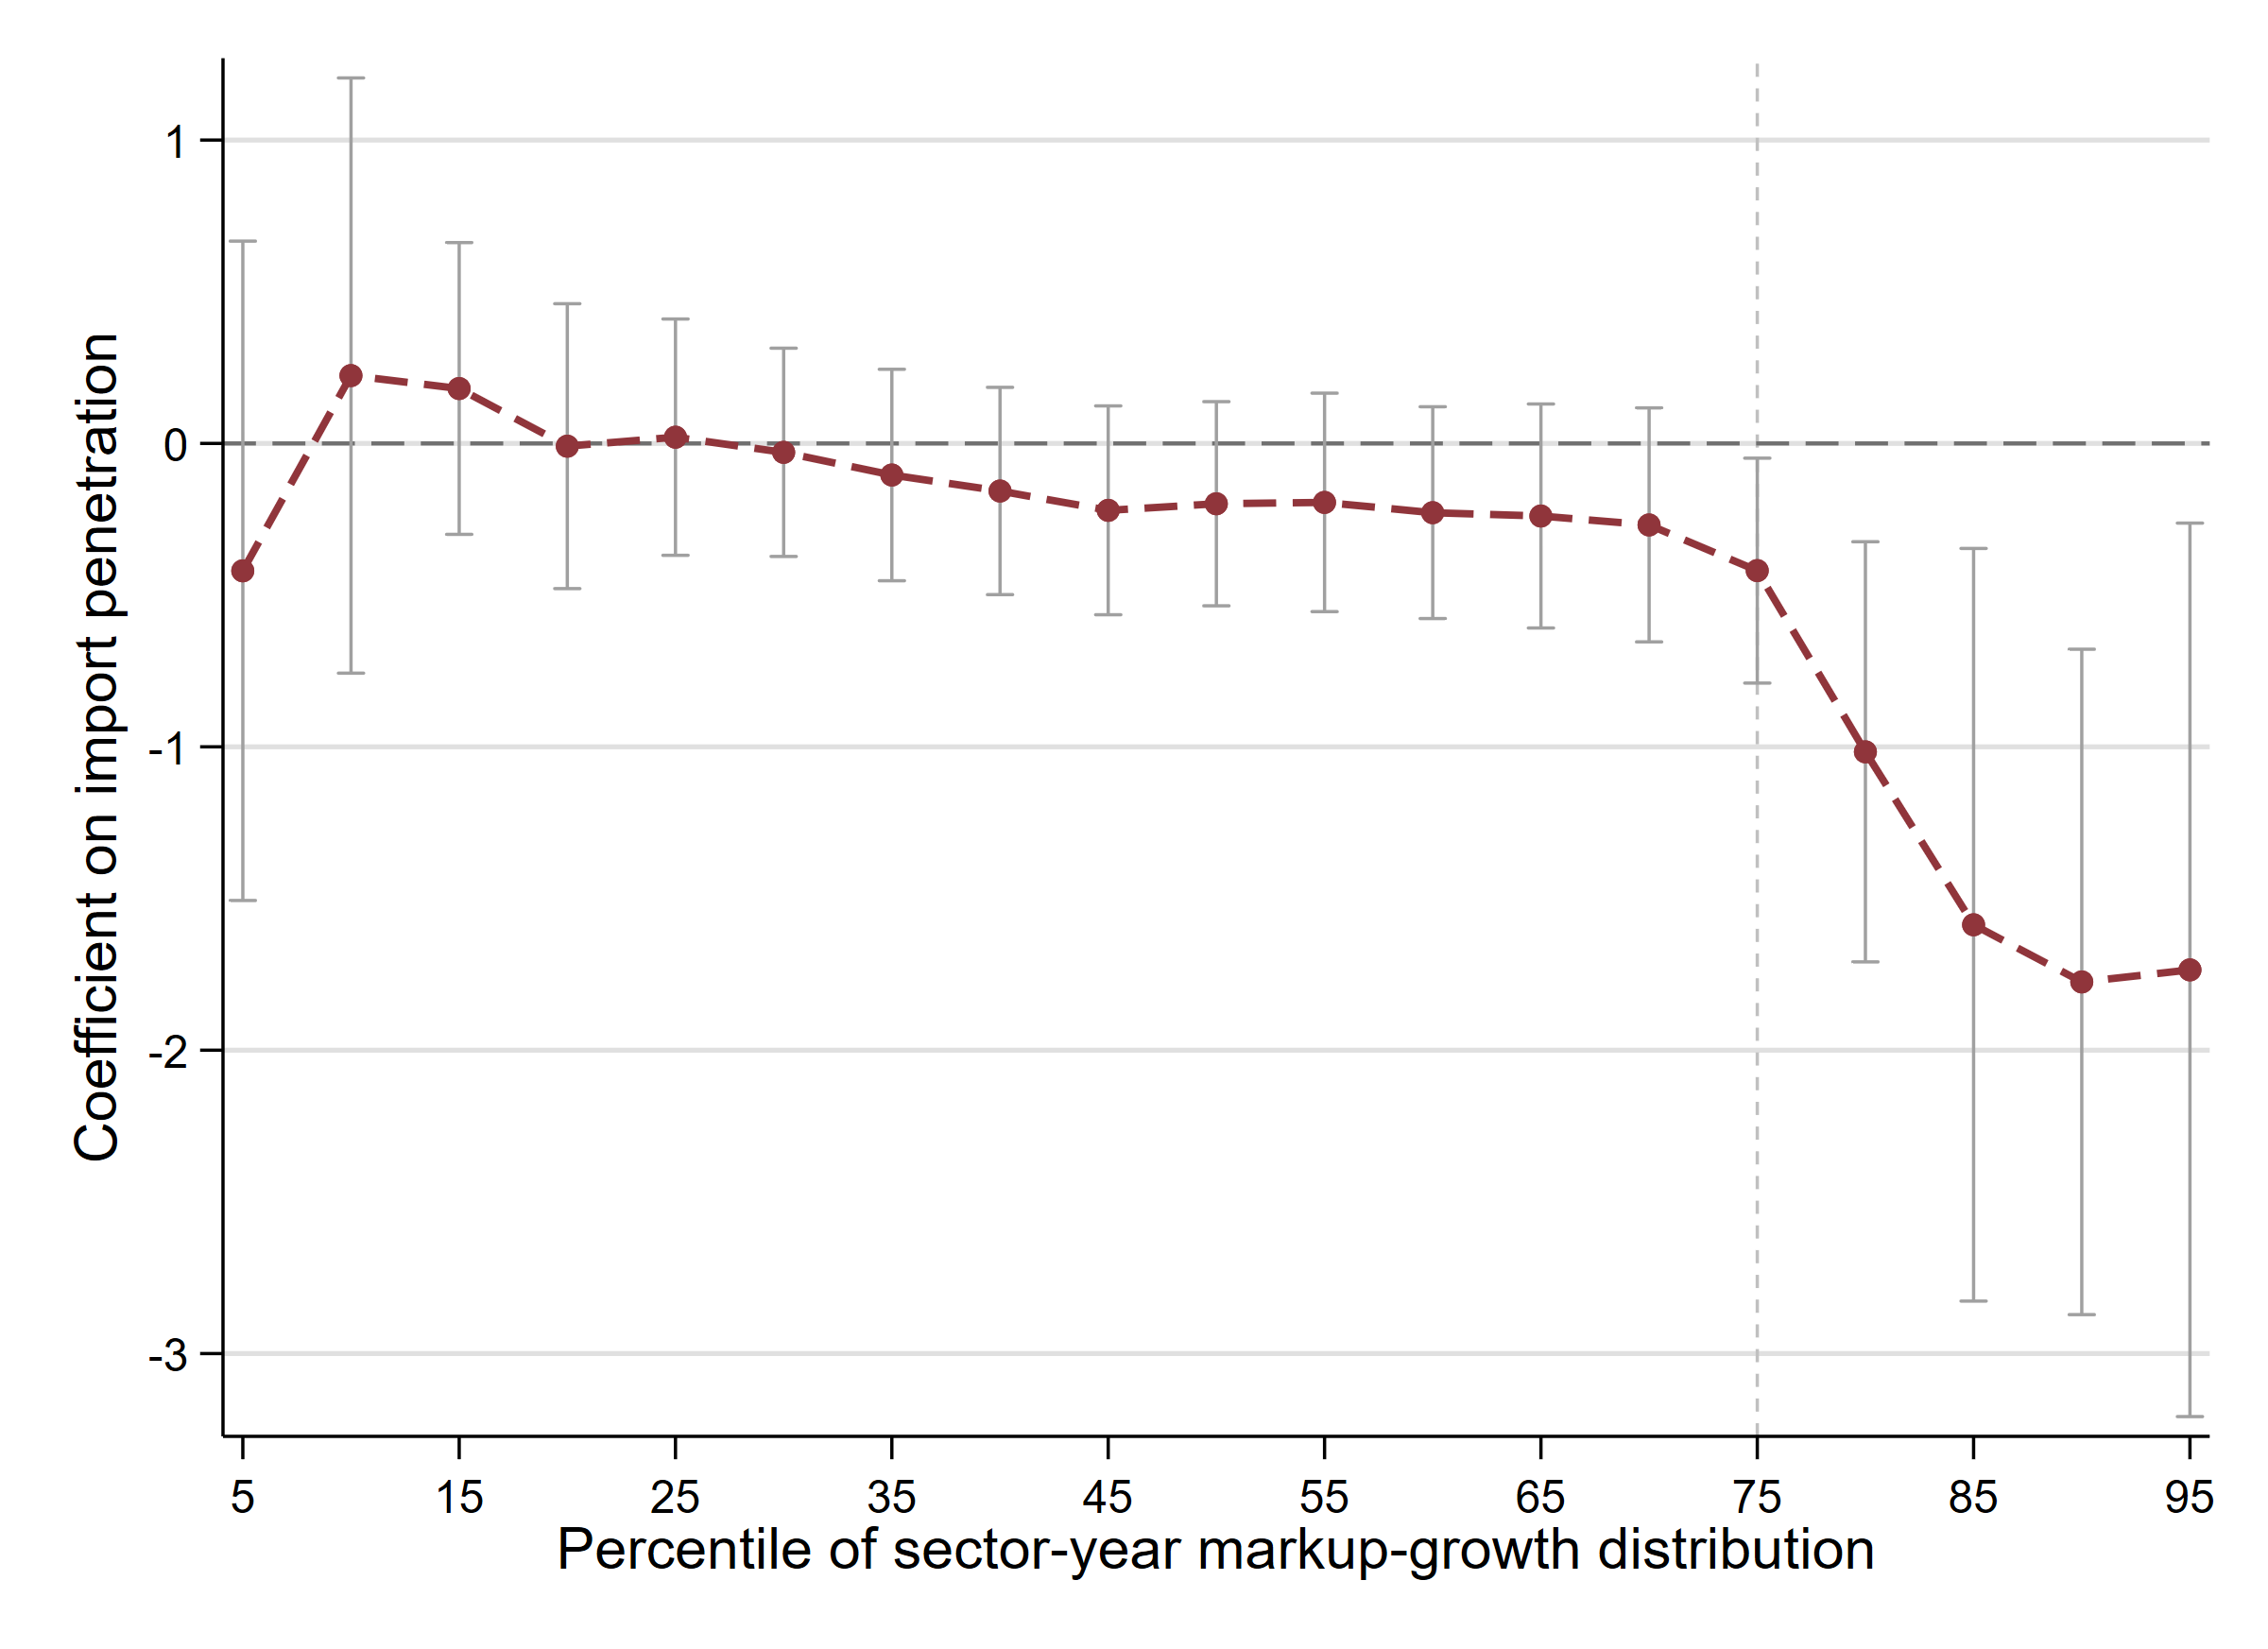
\includegraphics[width=0.85\textwidth]{iv_quantile_journal.png}
\caption[Grouped IV quantile estimates]{
Grouped IV quantile estimates for $\beta_O^{(k)}$ across sector-year deciles of the markup-adjustment distribution. Points report IV estimates; vertical bars report 95\% confidence intervals.
}
\label{fig:ivq_baseline}
\end{figure}

\begin{figure}[htbp]
\centering
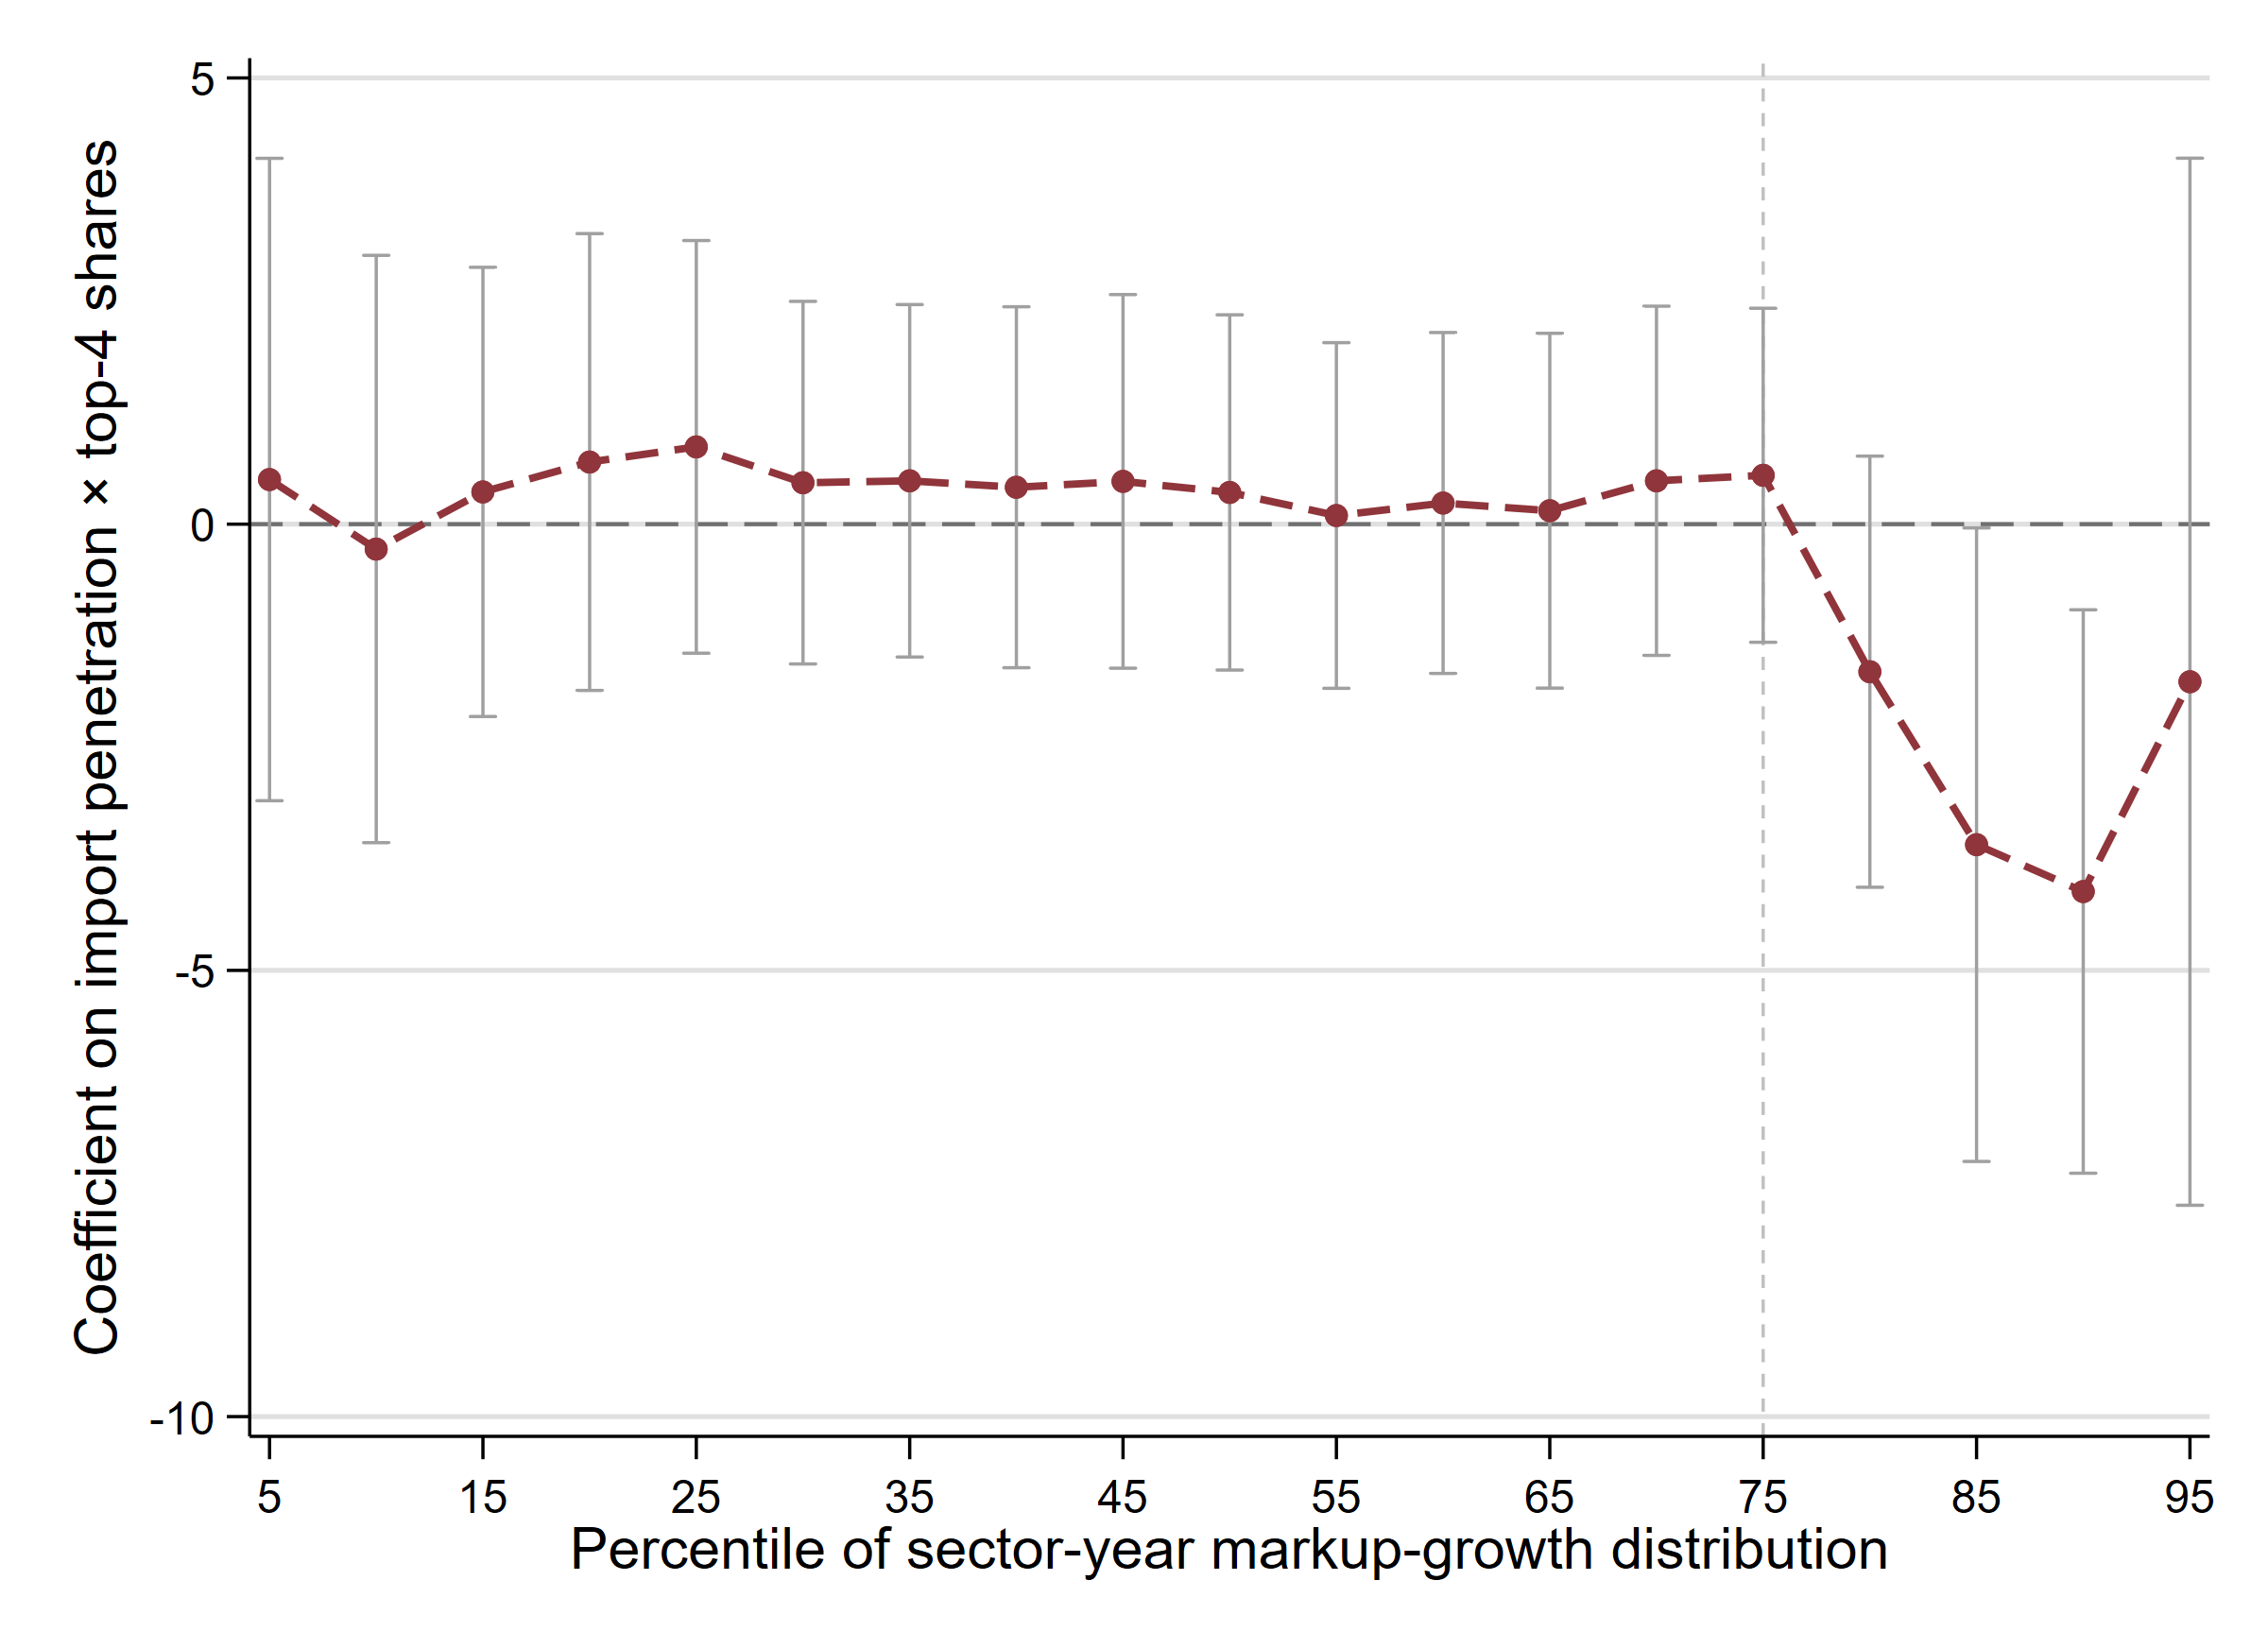
\includegraphics[width=0.85\textwidth]{iv_quantile_cr4_journal.png}
\caption[CR4 heterogeneity in grouped IV quantile estimates]{
Heterogeneity in grouped IV quantile estimates by pre-period domestic concentration. The figure reports interaction coefficients with CR4 across sector-year deciles, showing that negative upper-tail effects are stronger in more concentrated sectors.
}
\label{fig:ivq_cr4}
\end{figure}

This pattern suggests that import competition primarily constrains large positive markup adjustments in sector-year cells where the upper tail is moving up. In other words, the main within-incumbent discipline effect does not operate through a broad compression of all firms' pricing behavior, but through a disproportionate reduction in upper-tail markup growth. Firms in the center of the distribution, which are already making small or moderate markup adjustments, appear much less responsive to the trade shock. This finding is consistent with residual-demand discipline, but it should not be read mechanically as a statement that the baseline quantile exercise ranks firms by markup levels. The appendix check that ranks firms by lagged markup levels provides the closer test of that level-based interpretation. Because upper quantiles are sensitive to cell size, Appendix Tables~\ref{tab:mc_order_stat}--\ref{tab:mc_upper_tail_spline} report Monte Carlo diagnostics showing that the cell-size control and spline-bootstrap correction sharply reduce false rejection in the upper tail.

I next examine whether this upper-tail compression depends on domestic market structure. To do so, I interact import penetration with a measure of pre-period sectoral concentration, proxied by the domestic CR4 ratio. The estimates, reported in Figure \ref{fig:ivq_cr4}, show that the negative upper-tail effects are stronger in more concentrated sectors. The interaction coefficients remain close to zero in the lower and central quantiles, but become increasingly negative at high quantiles when concentration is high. This indicates that the compression of the markup-adjustment distribution is amplified in markets where a small number of firms account for a large share of domestic sales.

Taken together, these results support a mechanism in which import competition compresses the largest positive markup adjustments, especially in concentrated domestic industries. The evidence is therefore more consistent with targeted compression at the top of the markup-growth distribution than with a uniform decline in markups across all firms. This also helps reconcile the firm-level and sector-level results: even when average sectoral effects appear modest, import competition may still exert economically meaningful pro-competitive pressure by limiting upper-tail markup growth in the exposed cells that carry identifying weight.

\section{Threats to identification and robustness}

This section asks whether the two headline empirical claims survive the most relevant threats to interpretation. The first claim is that Chinese final-goods competition reduces markup growth among observed incumbent firms. The second is that this discipline is concentrated in the upper tail of the markup-adjustment distribution. I organize the checks around four questions. First, is the IV result driven by invalid pre-trends, omitted demand shocks, or a few influential sectors? Second, does the result depend on how markups or the firm sample are constructed? Third, is the upper-tail result an artifact of quantile construction? Fourth, can an oligopoly mechanism reproduce the same IV moments and absorb the residual output-shock variation?

\subsection{Identification: exposure, pre-trends, and influential sectors}

The first set of checks addresses the identifying variation behind the baseline IV. Table \ref{tab:rob12_fe} shows that the main coefficient is not driven by a narrow control set or functional-form choice. The preferred estimate is $-0.462$ and remains statistically significant under wild-cluster bootstrap inference. Removing lagged firm controls one block at a time leaves the coefficient close to the baseline: the estimates range from $-0.462$ with the preferred controls to $-0.396$ with no controls. Excluding the input-supply control also leaves a negative coefficient. The quadratic specification is less informative because the linear and squared terms are imprecise, but it provides no evidence that the baseline is hiding a strong nonlinear pattern.

The main identification caveat is not instability across controls; it is the concentration of identifying weight. Figure~\ref{fig:rotemberg_sector_size} and Appendix Table~\ref{tab:top_rotemberg_sector_size} show that the largest Rotemberg weights come from small but highly China-exposed cells. Table \ref{tab:rob_rotemberg_exclusions} confirms that these cells are central to the first stage: dropping the five largest-weight sectors lowers the F-statistic from 24.8 to 3.2, and broader exclusions make the second stage unstable. This does not invalidate the estimate, but it defines the estimand. The baseline result should be read as a local effect for influential exposed sectors, not as a homogeneous effect for all Turkish manufacturing. As an additional visual diagnostic, the synthetic-control exercise \parencite{abadieUsingSyntheticControls2021} for ISIC4 2790 shows a post-treatment deviation consistent with lower markup growth relative to a weighted counterfactual of lower-exposure sectors.

Two checks support the timing and exclusion assumptions on this support. Appendix Table~\ref{tab:pretrend_balance_outputIV} shows that future output-side China shocks do not predict pre-period trends in markups, revenue, or concentration. Appendix Table~\ref{tab:iv_demand_controls} adds high-income global-demand and Turkish export-demand controls; the import-penetration coefficient remains close to the baseline. Finally, because output-market and input-supply exposure are both built from China's trade growth, Appendix Tables \ref{tab:rob_resid_fs}--\ref{tab:rob_resid_aux} re-estimate the main specifications after residualizing \(Z^{\text{Output}}_{jt}\) with respect to \(Z^{\text{Input}}_{jt}\). The markup coefficient remains $-0.462$, with the same standard error and first-stage strength. The result therefore comes from the output-competition component of China exposure rather than from linear overlap with the upstream input channel.

\subsection{Markup measurement and sample selection}

The second set of checks examines whether the baseline result depends on the markup proxy or on the composition of the observed firm panel. Table~\ref{tab:kirov_iv} replaces the baseline COGS-based production-markup measure with the alternative procedure of \textcite{kirovMeasuringMarkupsRevenue2026} (KMT, henceforth). This is a demanding check because it requires lagged markup shifters and a Markov process for revenue productivity, which substantially reduces the usable sample. The estimated coefficient remains negative, but is imprecisely estimated. It shows that the sign survives a restrictive alternative markup construction, while the statistical precision of the baseline result relies on the larger COGS-based markup sample.

The remaining checks assess sample-composition sensitivity. Alternative trimming rules in Table~\ref{tab:rob_trimming} preserve the negative sign and the concentration of effects in the upper tail of the markup-adjustment distribution. Restricting the sample to longer-lived firms in Table~\ref{tab:rob_longlived} attenuates the coefficients, as expected when conditioning on surviving history. Product-level concentration within Chinese imports, reported in Appendix Tables~\ref{tab:rob_chn_gran_mean}--\ref{tab:rob_chn_gran_givq_foreign}, leaves the baseline coefficient essentially unchanged; the interaction estimates are imprecise and do not indicate that concentration across Chinese HS6 products drives the main result. Appendix Table~\ref{tab:mc_selection} reports finite-sample Monte Carlo diagnostics for the control-function selection procedure. This shows that the corrected specifications recover the imposed effect with negligible bias and close-to-nominal coverage, whereas the uncorrected specification is badly biased under endogenous observation.

Overall, these exercises support a narrow interpretation. The markup-disciplining effect is not an artifact of a single trimming rule, short-lived firms, or thin product cells. The sign stability across demanding measurement of markups and sample checks strengthens the interpretation of the baseline estimate as an incumbent markup response to output-market competition.

\subsection{Distributional design}

The third set of checks protects the upper-tail claim. The baseline grouped-IV quantile exercise ranks firms by markup adjustment within sector-year cells, so it could be sensitive to binning choices or small-cell order statistics. Appendix Figures \ref{fig:rob41_decquin}--\ref{fig:rob43_thin} address these concerns directly. Quintiles reproduce the same broad shape as deciles, and excluding thin sector-year cells leaves the upper-tail pattern visible.

The Monte Carlo evidence supports the baseline choice to control flexibly for cell size, and the targeted spline-bootstrap correction provides an additional upper-tail check. In a null design where sector-year cell size is correlated with the instrument, the uncorrected grouped-IV quantile estimator over-rejects heavily; Table \ref{tab:mc_order_stat} reports a false rejection rate of 69.4\% at Q90. Adding a baseline cubic polynomial in sector-year cell size lowers the Q90 rejection rate to 15.2\%. Furthermore, the targeted spline-bootstrap correction in Table \ref{tab:mc_upper_tail_spline} lowers it further to only 5\%.

\subsection{Internal consistency check}
\label{sec:smm_validation}

I implement a restricted SMM diagnostic to assess whether a parsimonious output-competition mechanism can reproduce the main IV moments within the model. The targeted moments are the baseline firm-level IV response, the grouped-IV upper-tail coefficients at Q80, Q85, and Q90, and the Q90 interaction with pre-period domestic concentration. The goal is to discipline the sign, magnitude, and concentration gradient of incumbent markup responses, not to provide independent structural validation of the key mechanisms.

\begin{table}[!htbp]
\centering
\caption{Targeted causal moment fit}
\label{tab:smm_fit_main}
\small
\begin{fittabular}{L{0.43\textwidth}rrrr}
\toprule
Target moment & Data & Model & Gap & Weight \\
\midrule
Baseline IV, \(\Delta\ln\mu\)  & -0.429 & -0.414 & -0.015 & 50.832 \\
Grouped IV, Q80 & -0.803 & -0.924 & 0.121 & 31.180 \\
Grouped IV, Q85 & -1.236 & -1.009 & -0.227 & 11.768 \\
Grouped IV, Q90 & -1.625 & -1.572 & -0.053 & 7.608 \\
Grouped IV, Q90 \(\times\) CR4 & -5.371 & -5.232 & -0.139 & 0.369 \\
\bottomrule
\end{fittabular}
\end{table}

Table~\ref{tab:smm_fit_main} shows that the restricted mechanism reproduces the central causal patterns in the data. The model matches the baseline IV response closely, captures the strong upper-tail discipline at Q90, and reproduces the sharper response in more concentrated sectors. The fit is less exact at Q80 and Q85, but the simulated moments preserve the empirical distributional shape: the markup response becomes increasingly negative toward the upper tail. The minimized criterion is \(Q=1.099\). Thus, the model is internally consistent with the targeted IV evidence.

As an absorption diagnostic, I subtract the model-implied output-competition component from incumbent markup growth and re-estimate the baseline IV regression on the residual, following the logic of \textcite{adaoPuttingQuantitativeModels2025}. After this targeted subtraction, the excluded output shifter has little remaining predictive content for residual markup growth: the coefficient falls to \(-0.052\), with a standard error of \(0.295\). Because the model is calibrated to moments that are close to the residualized regression, this result should be read as an internal-consistency check rather than as external validation.

The exercise is anchored on the strongest causal pattern in the paper: Chinese output competition lowers markup growth among observed incumbents, with the response concentrated in the upper tail and amplified in more concentrated sectors. Appendix~\ref{app:smm_indirect_inference} reports the parameter estimates, optimization details, residual-IV diagnostics, and non-targeted moments. Taken together, these checks strengthen the central contributions.


\section{Mechanism evidence and interpretation}
\label{sec:input_extension}

Mechanism evidence tests whether results reflect residual-demand discipline, input-cost relief, reallocation, or non-price adjustment. Tests are relegated to Appendix~\ref{app:mechanism_appendix}; the goal is interpretive consistency with baseline and sector-level results.

\textbf{Indirect residual-demand evidence.} To test residual-demand discipline, I interact instrumented import penetration with lagged firm markups and compare the implied marginal effects with the grouped-IV quantile evidence. Appendix Table~\ref{tab:mech_lagged_interactions} shows negative marginal effects at the 25th, 50th, and 75th percentiles of lagged markup, which partially supports the residual-demand effects.

\textbf{Input-cost relief and reallocation among continuing firms.} To separate cost relief from output discipline, I interact the input-supply shifter and output import penetration with pre-period Chinese imported-input dependence. Appendix Table~\ref{tab:input_dep_heterogeneity} shows a positive input-shock interaction in the markup regression, while the output interaction is imprecise. This supports a cost-relief channel.

I then test whether the shocks reallocate market share toward large or dominant incumbents. Appendix Table~\ref{tab:mech_share_reallocation} shows no significant output-shock reallocation toward large firms, while input-shock interactions are negative for size, large-firm status, and CR4 membership. This matches the sectoral decomposition: output competition mainly disciplines continuing firms, while input exposure reallocates shares among continuers without strengthening dominant survivors.

\textbf{Auxiliary outcomes.} As a final check, I estimate the same mechanism specifications for revenue, domestic sales, and exports. Appendix Table~\ref{tab:aux_outcomes} shows that import competition lowers revenue and domestic-sales growth, while export effects are imprecise. This supports the earlier interpretation: markup discipline comes with domestic demand pressure, not systematic export redirection.

\pagebreak
\section{Conclusion}

This thesis revisits the imports-as-market-discipline hypothesis in an emerging economy where domestic production is granular, firms are imperfectly competitive, and foreign exposure operates through both final-goods competition and imported-input linkages. Chinese final-goods competition disciplines markup growth among incumbent firms in exposed Turkish manufacturing sectors. The response is not a uniform downward shift: it is concentrated in the upper tail of markup adjustments and is stronger in more concentrated sectors, where residual-demand forces matter most. The selection diagnostic leaves the incumbent estimate unchanged after conditioning on lagged profitability, and the internal-consistency exercise supports an output-competition interpretation.

The aggregate result is more modest. Sector-level markup effects are weak and imprecise because within-firm discipline is partly offset by reallocation across continuing firms. Chinese input exposure behaves differently: it does not reduce within-firm markup growth but helps explain reallocation among input-dependent firms. Final-goods imports discipline incumbent pricing power; intermediate-input exposure reshapes cost positions and reallocates shares.

The development implication is that trade openness can weaken domestic market power inside concentrated industries—a channel especially relevant for emerging economies where incumbents dominate and domestic competition policy is institutionally limited. Yet trade exposure is an uneven instrument. The same exposure that limits pricing power can reduce domestic sales and survival. Lower markup growth may benefit consumers and downstream buyers, while workers, owners, and less productive firms bear adjustment costs. The evidence thus points to complementarity between trade openness and domestic competition policy, not substitution.

The main limitation is that accounting data miss welfare-relevant margins. Markups are estimated from revenue-based production methods rather than transaction-level price-cost margins; exit is disappearance from ORBIS/AMADEUS rather than validated legal death; and worker adjustment, consumer surplus, and input sourcing are unobserved. Future work should link accounting panels to administrative databases and matched worker records. These links would distinguish attrition from true exit, trace input-cost pass-through, measure employment adjustment, and test whether markup discipline reaches consumers—ultimately embedding this result in a general-equilibrium account of how import competition shapes market power and welfare in emerging economies.

\pagebreak

\printbibliography

\iffastcompile
\end{document}
\fi

\pagebreak

\appendix

\normalsize

\section{Theoretical appendix}
\label{app:theory_appendix}

\input{theopendix_selected.tex}

\subsection{From the static model to the first-difference specification}
\label{app:bridge}

This appendix bridges the static oligopoly model to the first-difference IV specification. Inverse markups are the natural theoretical object; annual log-markup changes provide local approximations to adjacent equilibria.

\subsubsection*{Local first-difference approximation}

Let the equilibrium markup of firm \(i\) in sector \(j\) and year \(t\) be written as
\[
\mu_{ijt}
=
M_j\!\left(\Lambda^D_{jt},\, s_{ijt},\, mc_{ijt};\, \theta_j\right),
\]
where \(\Lambda^D_{jt}\) is the domestic expenditure share, \(s_{ijt}\) is the relevant domestic market-share state, \(mc_{ijt}\) is marginal cost, and \(\theta_j\) collects demand and technology parameters. The closed-form markup condition in Section~\ref{sec:theory_model} is written in inverse-markup form. Since \(\log \mu_{ijt}=-\log \mu^{-1}_{ijt}\),
\[
\Delta \log \mu_{ijt}
=
-\Delta \log \mu^{-1}_{ijt}
\approx
-\frac{\Delta \mu^{-1}_{ijt}}{\mu^{-1}_{ij,t-1}}
=
-\mu_{ij,t-1}\Delta \mu^{-1}_{ijt}.
\]
Thus, for small annual changes, the sign predictions for changes in inverse markups translate directly into sign predictions for changes in log markups, with the opposite sign.

Define the local state vector $z_{ijt} = \big(\log \Lambda^D_{jt},\, s_{ijt},\, \log mc_{ijt}\big)$. A first-order expansion of \(\log M_j\) around the lagged equilibrium \(z_{ij,t-1}\) gives
\[
\Delta \log \mu_{ijt}
\approx
\psi_{\Lambda,ij,t-1}\Delta \log \Lambda^D_{jt}
+
\psi_{s,ij,t-1}\Delta s_{ijt}
+
\psi_{c,ij,t-1}\Delta \log mc_{ijt}
+
r_{ijt},
\]
where \(\psi\) are local derivatives and \(r_{ijt}\) collects higher-order terms. The empirical coefficient on a trade variable captures a local reduced-form equilibrium response combining the direct residual-demand effect with induced movement in market shares and marginal costs.

\subsubsection*{Mapping to the estimating equation}

The empirical design uses two observable trade-exposure measures to proxy for the theoretical state variables. Output-side Chinese import penetration proxies for changes in the domestic expenditure share:
\[
\Delta \log \Lambda^D_{jt}
=
\kappa_O \Delta IP_{jt}
+
\nu^O_{jt},
\qquad
\kappa_O<0.
\]
The input-supply shifter proxies for upstream cost exposure:
\[
\Delta \log mc_{ijt}
=
\kappa_I Z_{jt}^{\text{Input}}
+
\nu^I_{ijt}.
\]
Substituting these proxy mappings into the local expansion yields the baseline empirical analogue
\[
\Delta \log \hat\mu_{ijt}
=
\beta_O \Delta IP_{jt}
+
\beta_I Z_{jt}^{\text{Input}}
+
X'_{ijt-1}\gamma
+
\delta_j
+
\tau_t
+
\varepsilon_{ijt}.
\]
Here \(\beta_O\) is the local response of markup growth to output-market import competition, conditional on the input channel, lagged firm controls, sector fixed effects, and year fixed effects. The input coefficient \(\beta_I\) captures the separate reduced-form association between upstream exposure and markup growth.

Because \(\Delta IP_{jt}\) may respond to Turkish sectoral shocks, it is instrumented with the output-side shift-share variable. The input control is constructed from the same output shocks using predetermined input-output links, separating the excluded product-market competition shock from the observed upstream exposure channel. The resulting IV estimate is local to the sector-year cells that carry identifying weight in the shift-share design.

\subsubsection*{Selection and aggregation}

Selection can depend on latent profitability states affecting markup adjustment. Specification adds control-function in lagged EBIT margin. This yields within-incumbent response among survivors. Sectoral inverse markups aggregate linearly into within-firm, reallocation, entry, exit components.

\subsubsection*{Assumptions and scope}

Four conditions maintain interpretation: (1) annual changes small enough for Taylor remainder absorption; (2) sectoral parameters stable within window; (3) trade/input measures are informative proxies for theory; (4) conditional on fixed effects, Chinese export growth orthogonal to Turkish residual shocks. These define scope: design identifies relative exposure effects, not aggregate China effect. Coefficient weighted toward influential cells (Rotemberg weights).

\section{Empirical appendix}
\normalsize
\setlength{\textfloatsep}{0.55\baselineskip}
\setlength{\floatsep}{0.55\baselineskip}
\setlength{\intextsep}{0.55\baselineskip}
\setlength{\abovecaptionskip}{0.25\baselineskip}
\setlength{\belowcaptionskip}{0pt}

This appendix follows the order of the empirical sections in the main text. It first documents data construction and markup measurement, then reports supporting estimates for the empirical strategy and main results, then places robustness checks before the mechanism tables.

\subsection{Data, empirical strategy, and main results}

\subsubsection{Data}

\paragraph{ORBIS/AMADEUS firm panel.} The core microdata come from Bureau van Dijk company accounts. The project archive uses two raw Turkish extracts: a financial accounting file and a BvD industry classification file. The financial file contains harmonized balance-sheet, income-statement, and ratio variables, including operating revenue, costs of goods sold, tangible and intangible fixed assets, total assets, export revenue, debt, current assets and liabilities, working capital, interest expenses, cash holdings, EBIT margins, gross margins, and liquidity ratios. The classification file provides BvD firm identifiers and NACE Rev. 2 sector codes. I merge the two files by the BvD identifier and then retain the Turkish manufacturing panel after sector and deflator matches.

The cleaning procedure is designed to turn the raw accounting extract into a firm-year panel rather than a collection of filings. I date each observation by the fiscal closing date and keep one record per BvD firm-year. When more than one filing is available in the same year, the code gives priority to unconsolidated accounts before consolidated accounts, following the order U1, U2, C1, and C2. This matters because duplicate firm-years are often generated by consolidated and unconsolidated filings for the same legal entity. If the primary NACE code is unavailable, I use the secondary NACE code to reduce sector-code attrition. I then map firms from NACE Rev. 2 to 4-digit ISIC Rev. 4 sectors using the NACE--ISIC concordance used throughout the construction scripts.

Nominal ORBIS/AMADEUS accounting values are combined with TURKSTAT producer price indices before the main variables are constructed. The deflator is matched first at the 3-digit NACE level and, where needed, at the 2-digit NACE level. Observations without a usable manufacturing sector or without a matched PPI are dropped. The resulting raw Turkish manufacturing panel used in the thesis covers 15,957 firms and 78,921 firm-year observations from 2009 to 2023. The panel is unbalanced: firms can enter the observed sample, disappear, or report intermittently. I do not impute missing accounting years. For this reason, the thesis interprets disappearance from ORBIS/AMADEUS as observed sample turnover rather than validated legal closure or economic exit.

\begin{figure}[!htbp]
    \centering
    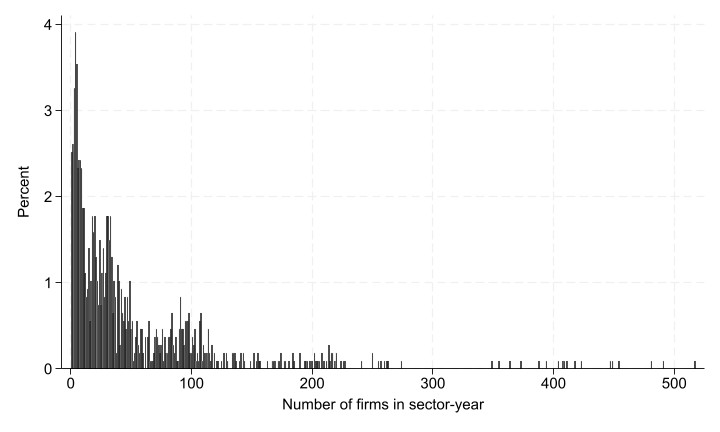
\includegraphics[width=0.86\textwidth]{sector_size_distribution.jpg}
    \caption[Distribution of sector-year cell sizes]{Distribution of sector-year cell sizes. The horizontal axis is the number of firms in an ISIC4 sector-year cell and the vertical axis is percent.}
    \label{fig:data_sector_size}
\end{figure}

The firm-level outcome construction follows the same panel logic. Revenue, costs of goods sold, tangible fixed assets, intangible fixed assets, and domestic sales are deflated by the matched PPI. Domestic sales are calculated as operating revenue minus export revenue when export revenue is available. Sector-year domestic market shares are then computed within 4-digit ISIC sectors, and these shares are used to build concentration measures such as CR10, CR20, the domestic HHI, and the firm-count variables used in the heterogeneity and decomposition exercises. Firm age is measured as years since the first observed year in the ORBIS/AMADEUS panel, so it is a panel-age measure rather than a legal incorporation-age measure. Other controls and mechanisms are built from lagged accounting ratios, including firm size, leverage, liquidity, current ratio, working-capital intensity, interest burden, and cash buffers.

Tables~\ref{tab:orbis_coverage_appendix} and \ref{tab:domestic_sales_export_audit} report two data-quality checks behind this construction. Table~\ref{tab:orbis_coverage_appendix} compares aggregate ORBIS operating revenue with UNIDO INDSTAT4 output at the ISIC4-year level over 2011--2019. ORBIS covers a meaningful but incomplete share of official output: median coverage is about 19--20 percent in the two lowest China-exposure quartiles and about 33--38 percent in the two higher quartiles. The pattern supports using ORBIS as a firm-panel source for within-firm and within-sector variation, but it also rules out interpreting the raw ORBIS panel as a complete census of Turkish manufacturing output.

\begin{table}[!htbp]\centering
\caption{ORBIS coverage relative to official sector output}
\label{tab:orbis_coverage_appendix}
\begin{tabular}{lrrrrrr}
\toprule
China exposure quartile & Mean & p25 & Median & p75 & Sector-years & ORBIS firms \\
\midrule
Q1: lowest & 0.232 & 0.139 & 0.193 & 0.290 & 203 & 54.9 \\
Q2 & 0.273 & 0.102 & 0.198 & 0.345 & 187 & 106.3 \\
Q3 & 0.644 & 0.217 & 0.380 & 0.537 & 190 & 97.8 \\
Q4: highest & 0.695 & 0.170 & 0.333 & 0.575 & 177 & 40.1 \\
\bottomrule
\end{tabular}
\begin{minipage}{0.92\textwidth}
\vspace{0.3em}\footnotesize Notes: Coverage is the ISIC4-year ratio of aggregate ORBIS operating revenue/turnover to official sector output from UNIDO ISDB/INDSTAT. The compact display reports distributions by 2009 China-exposure quartile. Because ORBIS accounting values and official output differ in source coverage, currency conversion, and reporting conventions, the ratio is a coverage diagnostic.
\end{minipage}
\end{table}


Table~\ref{tab:domestic_sales_export_audit} focuses on the accounting object used for domestic sales. Missing export revenue is not the same as zero export revenue. During the 2011--2019 baseline window, the missing-export share is modest in 2011 and 2016--2019, but it rises sharply in 2013--2015, reaching 42.5 percent in 2015. I therefore construct domestic sales only when export revenue is observed and treat domestic-sales-based concentration and auxiliary domestic-sales outcomes as measurement-sensitive objects, not as direct administrative totals.

\begin{table}[!htbp]\centering
\caption{Audit of export revenue used to construct domestic sales}
\label{tab:domestic_sales_export_audit}
\begin{tabular}{lrrrr}
\toprule
Group & Firm-years & Missing exports (\%) & Zero exports (\%) & Positive exports (\%) \\
\midrule
\multicolumn{5}{l}{Panel A: By year} \\
2011 & 6,522 & 5.7 & 34.2 & 60.2 \\
2012 & 7,682 & 13.3 & 32.4 & 54.3 \\
2013 & 8,847 & 24.7 & 26.3 & 49.0 \\
2014 & 9,517 & 33.1 & 22.3 & 44.6 \\
2015 & 10,806 & 42.5 & 19.2 & 38.3 \\
2016 & 6,767 & 9.0 & 29.7 & 61.3 \\
2017 & 6,542 & 5.7 & 29.5 & 64.8 \\
2018 & 6,696 & 9.0 & 28.1 & 62.9 \\
2019 & 6,769 & 9.1 & 26.3 & 64.6 \\
\midrule
\multicolumn{5}{l}{Panel B: By two-digit ISIC sector, 2011--2019} \\
10 & 5,913 & 16.1 & 39.3 & 44.6 \\
11 & 281 & 29.2 & 30.2 & 40.6 \\
12 & 55 & 16.4 & 7.3 & 76.4 \\
13 & 7,315 & 21.1 & 23.4 & 55.5 \\
14 & 4,135 & 20.2 & 24.1 & 55.7 \\
15 & 863 & 18.2 & 29.2 & 52.6 \\
16 & 1,264 & 17.2 & 37.0 & 45.8 \\
17 & 3,134 & 16.1 & 26.5 & 57.4 \\
18 & 1,480 & 17.6 & 46.9 & 35.5 \\
19 & 359 & 19.2 & 34.0 & 46.8 \\
20 & 5,825 & 18.6 & 21.5 & 59.8 \\
21 & 382 & 29.8 & 23.6 & 46.6 \\
22 & 6,354 & 18.1 & 25.1 & 56.8 \\
23 & 3,132 & 20.6 & 39.4 & 40.0 \\
24 & 3,664 & 17.2 & 22.2 & 60.5 \\
25 & 7,161 & 20.1 & 28.5 & 51.5 \\
26 & 1,148 & 20.4 & 22.0 & 57.6 \\
27 & 2,648 & 19.5 & 25.9 & 54.5 \\
28 & 7,238 & 19.1 & 20.7 & 60.1 \\
29 & 2,713 & 18.9 & 16.4 & 64.7 \\
30 & 641 & 23.9 & 23.4 & 52.7 \\
31 & 2,254 & 24.2 & 29.8 & 46.0 \\
32 & 2,189 & 22.2 & 28.1 & 49.7 \\
\bottomrule
\end{tabular}
\begin{minipage}{0.92\textwidth}
\vspace{0.3em}\footnotesize Notes: The sample is restricted to the 2011--2019 baseline IV window. Domestic sales are mechanically observed only when operating revenue and export revenue are both observed. Missing export revenue is not treated as zero exports.
\end{minipage}
\end{table}


Figure \ref{fig:data_number_firms} documents the evolution of the number of observed firms over time. The decline in coverage in later years is one reason why the main text treats ORBIS/AMADEUS disappearance cautiously and why the baseline regressions control for pre-period labor intensity interacted with the post-2016 period. Figure \ref{fig:data_sector_size} summarizes the distribution of sector size in the manufacturing sample and illustrates the granularity behind the shift-share design.

\begin{figure}[!htbp]
    \centering
    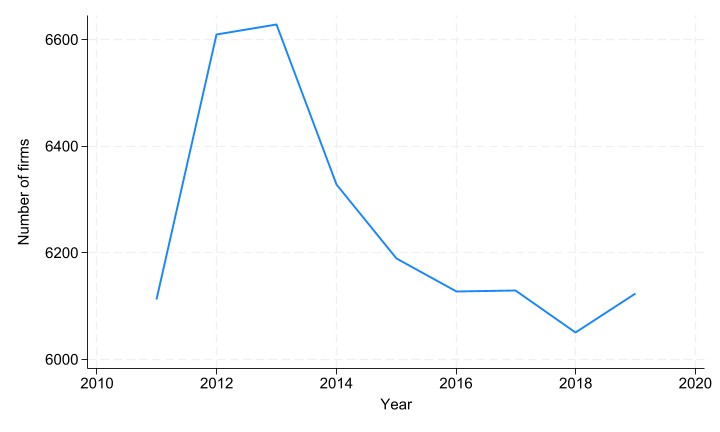
\includegraphics[width=0.86\textwidth]{number_firms_over_time.jpg}
    \caption[Observed firms over time]{Observed ORBIS/AMADEUS manufacturing firms by year. The horizontal axis is year and the vertical axis is the number of observed firms.}
    \label{fig:data_number_firms}
\end{figure}

\paragraph{CEPII BACI trade data.} CEPII BACI HS96 files provide bilateral trade flows at the HS 6-digit level. In the import-penetration construction, I keep Chinese exports to Turkey, using China as exporter code 156 and Turkey as importer code 792, and aggregate product flows to ISIC Rev. 4 manufacturing sectors. The baseline treatment is
\[
IP_{jt}=\frac{M^{CHN\rightarrow TUR}_{jt}}{\text{Apparent consumption}_{jt}},
\]
and the regressor used in the firm-level specifications is the annual change in this sectoral import-penetration rate. The BACI files are also used for the shift-share design. The exposure share is based on China's 2009 exports to Turkey by sector relative to sectoral absorption. The shift component is the change in China's export performance in other high-income destinations, including the United States, Japan, South Korea, Australia, and EU-15 economies. A separate BACI construction over 2000--2004 is used in the mechanism section to measure China's pre-period share in Turkey's upstream imports.

\paragraph{UNIDO sector data.} UNIDO ISDB/INDSTAT4 files provide sectoral manufacturing aggregates at the 4-digit ISIC level. I use Turkish sectoral output and apparent consumption to construct the denominator of import penetration and the 2009 exposure shares. The construction scripts import Turkish output from the UNIDO file, harmonize sector codes to ISIC Rev. 4, and use the ISDB apparent-consumption series directly when computing import penetration for 2011--2019. A high-income import file is also used to normalize the high-income-destination shift in the output-competition instrument.

\paragraph{WIOD input-output data.} The input-supply shifter is built from the Turkish national input-output table in WIOD. The main construction uses the 2003 table. I keep domestic and imported intermediate-flow rows, drop final-demand and total rows, reshape the table into input-sector by using-sector cells, and compute
\[
w_{jk}=\frac{\text{intermediate purchases by sector }j\text{ from sector }k}{\text{total intermediate purchases by sector }j}.
\]
Manufacturing using sectors are retained, while the denominator includes all intermediate inputs rather than only manufacturing inputs. The output-side sector shock is then propagated through this fixed input-output matrix to obtain the input-supply control $Z^{\text{Input}}_{jt}=\sum_k w_{jk}Z^{\text{Output}}_{kt}$. For the imported-input-dependence mechanism, I also use 2000--2004 WIOD weights and combine them with BACI-based Chinese import shares in upstream sectors.

\paragraph{TURKSTAT data.} TURKSTAT data enter in two places. First, the monthly sectoral Producer Price Index is converted into annual sectoral PPI series and used to deflate ORBIS/AMADEUS accounting variables. The construction uses 3-digit NACE deflators where available and falls back to 2-digit deflators otherwise. Second, TURKSTAT Annual Industry and Service Statistics extracts on personnel costs and value added at factor cost are used to construct sectoral labor intensity. I compute the ratio of personnel costs to value added, average it over the pre-2016 period, fill missing 4-digit values with 3-digit or 2-digit sector means when necessary, and map the resulting measure to ISIC Rev. 4. This time-invariant labor-intensity control is interacted with a post-2016 dummy in the baseline specifications.

\paragraph{HS96--ISIC Rev. 4 concordance.}\hfill\par
\label{app:hs_isic_concordance}
\noindent The HS-ISIC package \parencite{liaoConcordanceProductConcordance2020} supports HS revisions, ISIC Rev. 2, Rev. 3, Rev. 3.1, and Rev. 4, and reports all destination matches and occurrence-share weights. The HS96-to-ISIC4 bridge is many-to-many. The package first uses the HS96-to-ISIC Rev. 3 dictionary and then links ISIC Rev. 3 to ISIC Rev. 4; after retaining distinct matched pairs, it counts how often each 4-digit ISIC destination occurs for a given HS product and converts these counts into shares. For each BACI observation, trade value is therefore split across matched industries as $X_{hjt}=s_{hj}X_{ht}$, where $h$ is the HS96 6-digit product, $j$ is the ISIC Rev. 4 sector, and $\sum_j s_{hj}=1$ over the matched sectors for product $h$. The allocated values are then collapsed to sector-year totals before constructing import penetration, the shift-share exposure, and the Chinese product-granularity robustness measure.

\subsubsection{Markup estimation}
\label{app:markup_estimation}

\textbf{Baseline estimator}: I estimate firm markups using the production approach in \textcite{deloeckerMarkupsFirmLevelExport2012,deloeckerRiseMarketPower2020}, with the implementation guided by \textcite{deridderHitchhikersGuideMarkup2026}. The baseline uses COGS as the flexible input because it is the most consistently observed variable input in ORBIS/AMADEUS. For firm \(i\) in year \(t\), let \(r_{it} = \log R_{it}, x_{it} = \log X_{it}, k_{it} = \log K_{it}\), where \(R_{it}\) is revenue, \(X_{it}\) is COGS, and \(K_{it}\) is capital. The estimation sample requires \(R_{it}>0\), \(X_{it}>0\), and \(K_{it}>0\).

\textbf{Markup recovery}: For a flexible input, the first-order condition implies
\[
\mu_{it}
=
\theta_{it}^{\text{COGS}} \frac{R_{it}}{X_{it}},
\]
where \(\theta_{it}^{\text{COGS}}\) is the output elasticity of COGS. In logs, the empirical markup is therefore
\[
\log \hat{\mu}_{it}
=
\log \hat{\theta}_{it}^{\text{COGS}}
+ \log R_{it}
- \log X_{it}.
\]
The main empirical outcome is \(\Delta \log \hat{\mu}_{it}\) rather than the level \(\log \hat{\mu}_{it}\). This choice is deliberate: markup levels inferred from accounting data are more exposed to persistent reporting differences, production-function misspecification, and denominator error, whereas within-firm changes are better aligned with the time variation in the import-competition shock.

\textbf{Translog sensitivity}: In the baseline implementation, I allow the flexible-input elasticity to vary with input levels by estimating a two-input translog specification:
\[
r_{it}
=
\beta_x x_{it}
+ \beta_k k_{it}
+ \beta_{xx} x_{it}^2
+ \beta_{kk} k_{it}^2
+ \beta_{xk}x_{it}k_{it}
+ \lambda_t
+ \varepsilon_{it}.
\]
The implied firm-year COGS elasticity is then
\[
\hat{\theta}_{it}^{\text{COGS}}
=
\frac{\partial r_{it}}{\partial x_{it}}
=
\hat{\beta}_x
+ 2\hat{\beta}_{xx}x_{it}
+ \hat{\beta}_{xk}k_{it}.
\]

\subsubsection{Grouped-IV quantile estimates}
\renewcommand{\arraystretch}{0.9}

Tables \ref{tab:givq_panel_a} and \ref{tab:givq_panel_b} report the numerical grouped-IV quantile estimates underlying Figure \ref{fig:ivq_baseline}. The outcome in each column is the corresponding sector-year quantile of firm-level markup adjustment, and the treatment remains instrumented sectoral import-penetration growth.

\begin{table}[htbp]\centering
\def\sym#1{\ifmmode^{#1}\else\(^{#1}\)\fi}
\caption{Grouped IV quantiles of markup adjustment (Panel A: p5--p50)}
\label{tab:givq_panel_a}
\setlength{\tabcolsep}{2pt}
\begin{fittabular}{L{0.25\textwidth}*{10}{c}}
\hline\hline
            &\multicolumn{1}{c}{q5}&\multicolumn{1}{c}{q10}&\multicolumn{1}{c}{q15}&\multicolumn{1}{c}{q20}&\multicolumn{1}{c}{q25}&\multicolumn{1}{c}{q30}&\multicolumn{1}{c}{q35}&\multicolumn{1}{c}{q40}&\multicolumn{1}{c}{q45}&\multicolumn{1}{c}{q50}\\
\hline
Import penetration  &      -0.531         &       0.154         &       0.245         &    -0.00378         &      0.0130         &     -0.0290         &     -0.0971         &      -0.158         &      -0.223         &      -0.195         \\
            &     (0.506)         &     (0.429)         &     (0.207)         &     (0.217)         &     (0.185)         &     (0.160)         &     (0.160)         &     (0.154)         &     (0.156)         &     (0.141)         \\
[0.2em]
Input-supply shock     &       5.836\sym{*}  &       3.821         &       0.800         &     -0.0735         &      -0.396         &      -0.334         &      0.0461         &      0.0166         &      0.0383         &      0.0150         \\
            &     (3.339)         &     (2.725)         &     (1.229)         &     (0.694)         &     (0.648)         &     (0.628)         &     (0.550)         &     (0.526)         &     (0.506)         &     (0.489)         \\
\hline
Observations &         609         &         609         &         609         &         609         &         609         &         609         &         609         &         609         &         609         &         609         \\
\hline\hline
\multicolumn{11}{l}{\footnotesize Notes: Each dependent variable is the indicated sector-year quantile of firm-level markup adjustment.}\\
\multicolumn{11}{l}{\footnotesize Standard errors in parentheses. Specifications include sector and year fixed effects, controls, and a cubic in cell size.}\\
\multicolumn{11}{l}{\footnotesize \sym{*} \(p<0.10\), \sym{**} \(p<0.05\), \sym{***} \(p<0.01\)}\\
\end{fittabular}
\end{table}

\begin{table}[htbp]\centering
\def\sym#1{\ifmmode^{#1}\else\(^{#1}\)\fi}
\caption{Grouped IV quantiles of markup adjustment (Panel B: p55--p95)}
\label{tab:givq_panel_b}
\setlength{\tabcolsep}{2pt}
\begin{fittabular}{L{0.25\textwidth}*{9}{c}}
\hline\hline
            &\multicolumn{1}{c}{q55}&\multicolumn{1}{c}{q60}&\multicolumn{1}{c}{q65}&\multicolumn{1}{c}{q70}&\multicolumn{1}{c}{q75}&\multicolumn{1}{c}{q80}&\multicolumn{1}{c}{q85}&\multicolumn{1}{c}{q90}&\multicolumn{1}{c}{q95}\\
\hline
Import penetration  &      -0.182         &      -0.219         &      -0.235         &      -0.108         &      -0.246         &      -0.848\sym{***}&      -1.423\sym{**} &      -1.585\sym{***}&      -1.462\sym{*}  \\
            &     (0.148)         &     (0.147)         &     (0.158)         &     (0.148)         &     (0.160)         &     (0.313)         &     (0.597)         &     (0.550)         &     (0.748)         \\
[0.2em]
Input-supply shock     &      -0.176         &      0.0432         &       0.141         &       1.474         &       1.476         &       1.465         &       1.782         &       1.709         &       6.899\sym{**} \\
            &     (0.504)         &     (0.559)         &     (0.592)         &     (1.560)         &     (1.563)         &     (1.757)         &     (2.125)         &     (2.215)         &     (3.199)         \\
\hline
Observations &         609         &         609         &         609         &         609         &         609         &         609         &         609         &         609         &         609         \\
\hline\hline
\multicolumn{10}{l}{\footnotesize Notes: Each dependent variable is the indicated sector-year quantile of firm-level markup adjustment.}\\
\multicolumn{10}{l}{\footnotesize Standard errors in parentheses. Specifications include sector and year fixed effects, controls, and a cubic in cell size.}\\
\multicolumn{10}{l}{\footnotesize \sym{*} \(p<0.10\), \sym{**} \(p<0.05\), \sym{***} \(p<0.01\)}\\
\end{fittabular}
\end{table}

\begin{figure}[htbp]
\centering
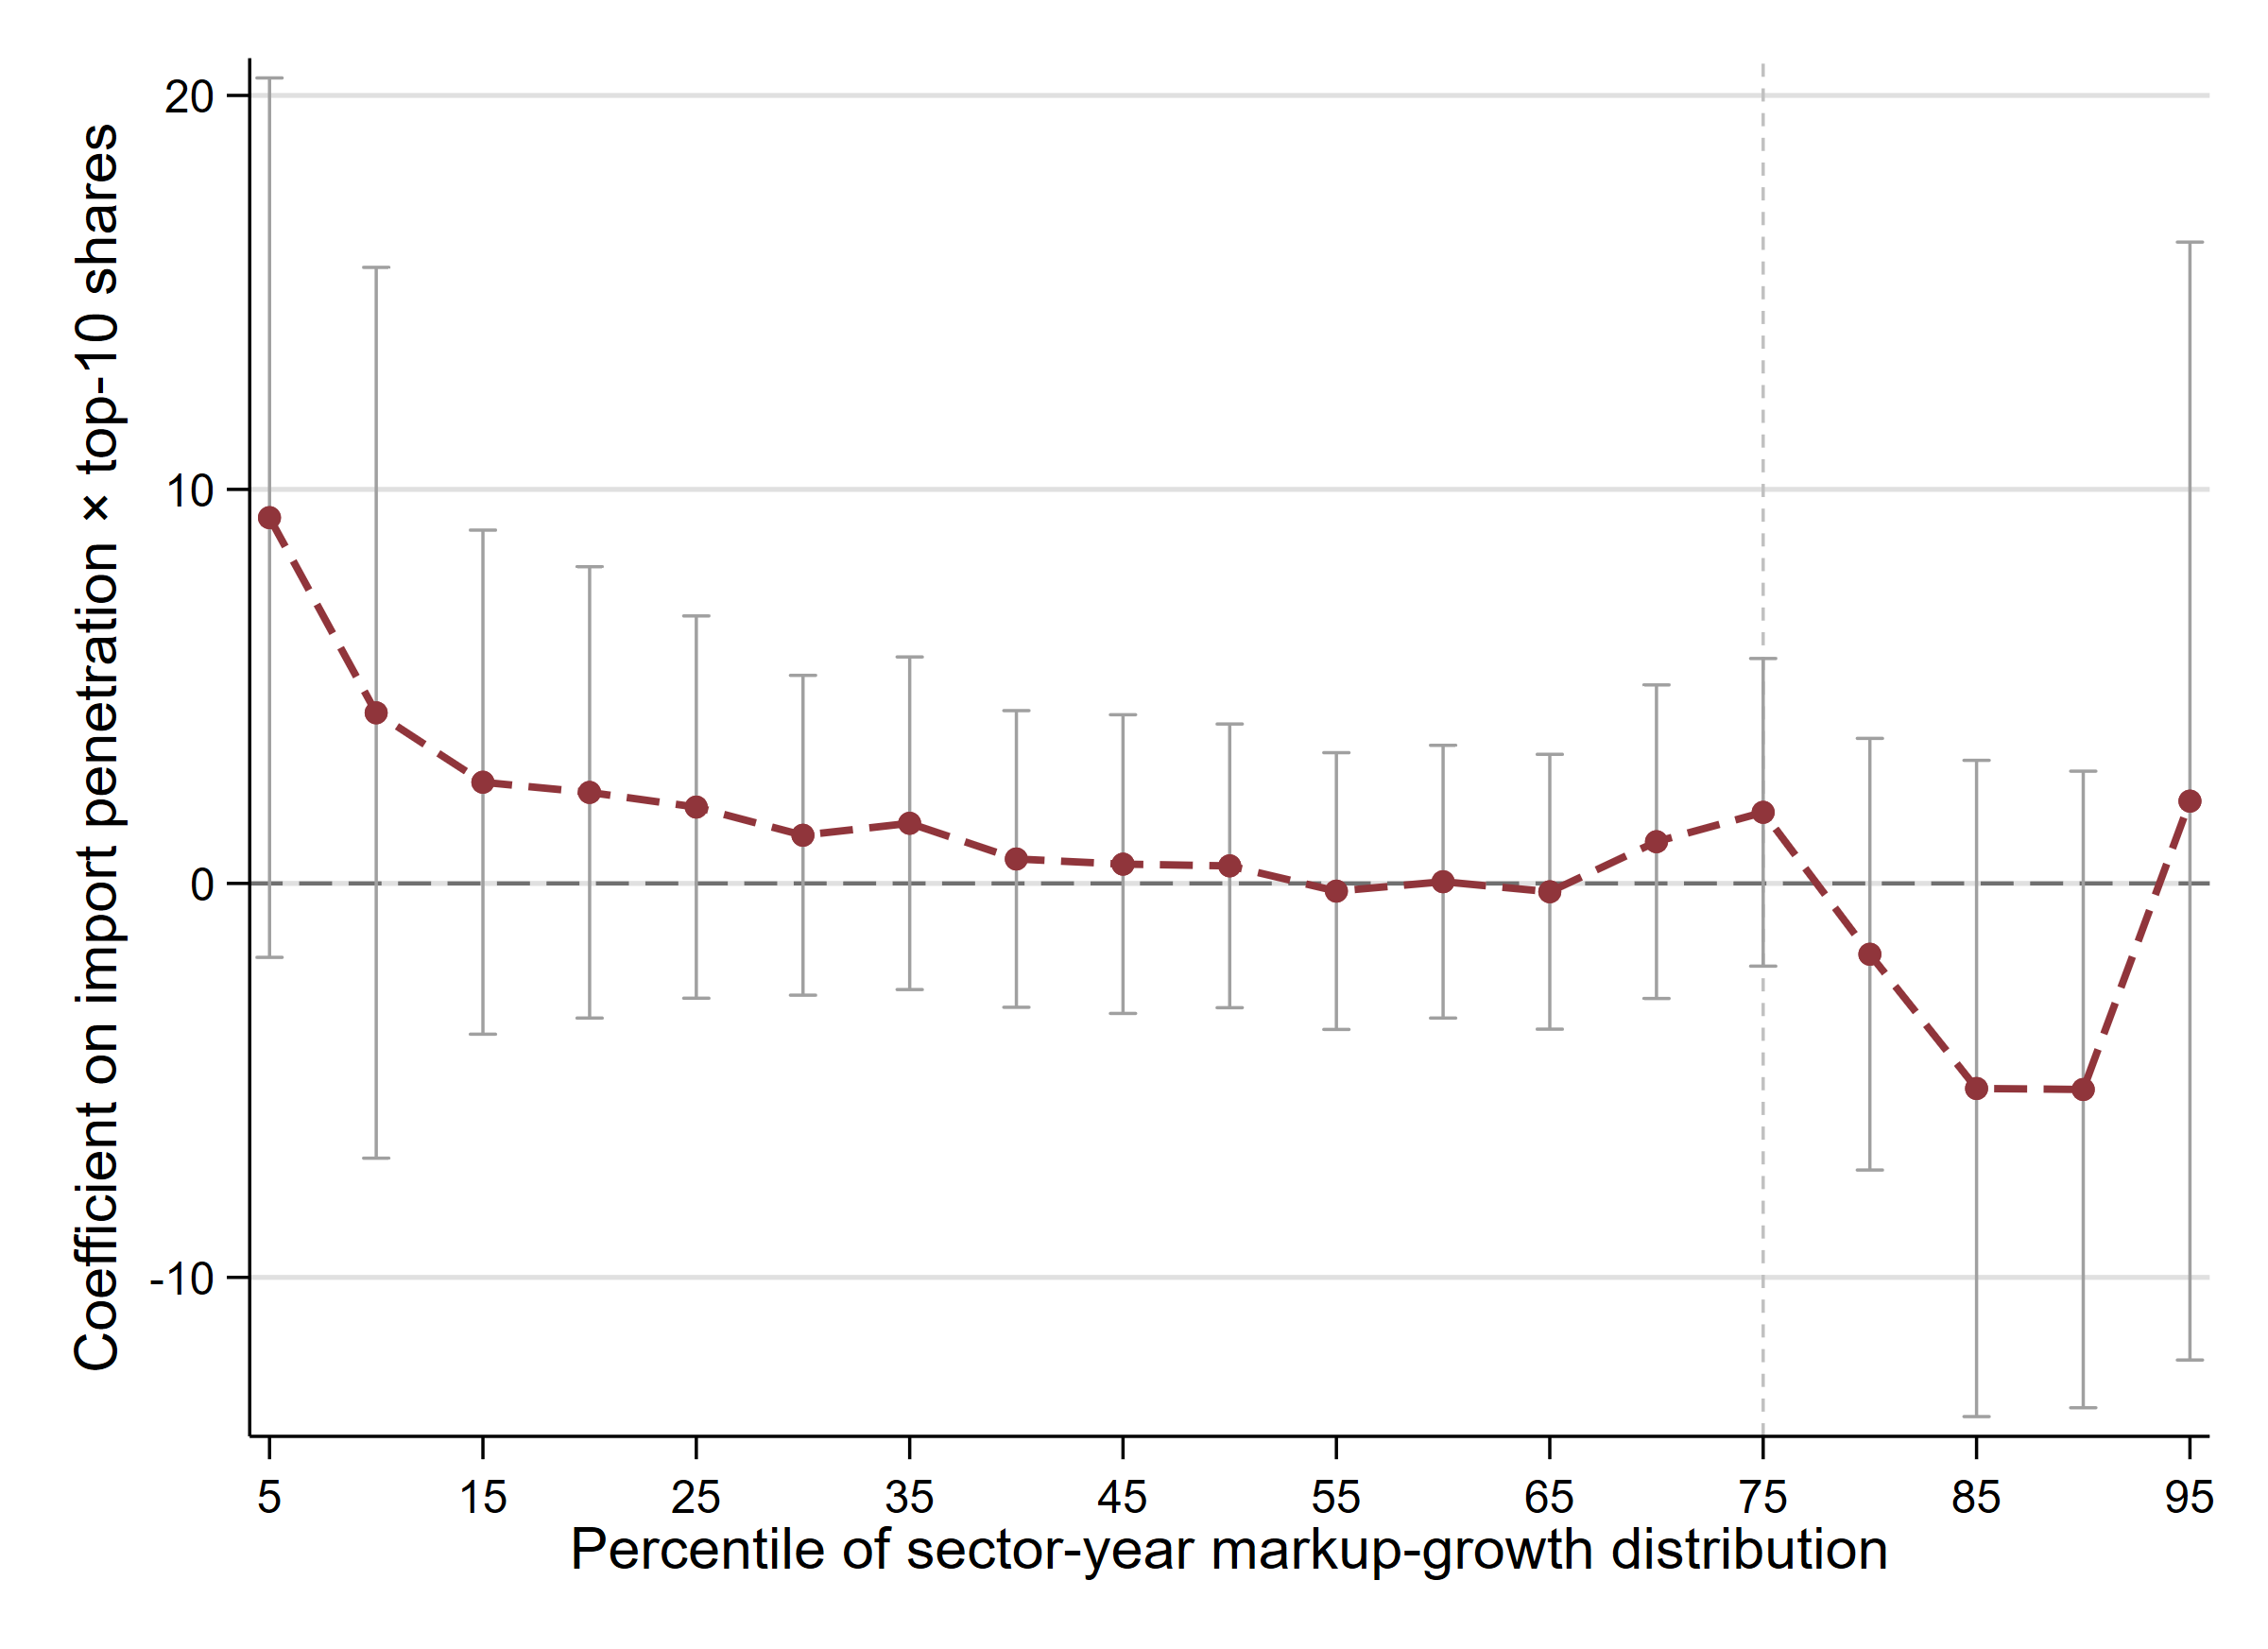
\includegraphics[width=0.85\textwidth]{iv_quantile_cr10_journal.png}
\caption[CR10 heterogeneity in grouped IV quantile estimates]{
Heterogeneity in grouped IV quantile estimates by pre-period domestic concentration. The figure reports interaction coefficients with CR10 across sector-year deciles, showing that negative upper-tail effects appear in more concentrated sectors.
}
\label{fig:ivq_cr10}
\end{figure}

\subsection{Threats to Identification and Robustness}

\subsubsection{Control-set sensitivity}

Table~\ref{tab:rob12_fe} reports specification checks varying controls, excluding input-supply shock, and adding quadratic terms. Output-competition coefficient remains negative across linear specs.

\begin{table}[!htbp]
\centering
\def\sym#1{\ifmmode^{#1}\else\(^{#1}\)\fi}
\caption{Specification diagnostics: functional form and control-set sensitivity}
\label{tab:rob12_fe}
\small
\setlength{\tabcolsep}{4pt}
\renewcommand{\arraystretch}{1.12}
\begin{fittabular}{L{0.08\textwidth}L{0.17\textwidth}L{0.16\textwidth}L{0.16\textwidth}c c c L{0.28\textwidth}}
\toprule
Spec & Output-shock effect ($\Delta IP$) & Input-shock control ($Z^{\text{Input}}$) & Quadratic term ($\Delta IP^2$) & Obs. & Wild p-value & ID & Control-set design \\
\midrule
S1 & -0.462\sym{**} (0.226) & 0.517 (0.470) & -- & 30551 & 0.026 & (1) & Baseline \\
S2 & -0.101 (0.485) & 0.578 (0.391) & 7.783 (6.489) & 30551 & . & (2) & Quadratic \\
S3 & -0.462\sym{**} (0.226) & 0.518 (0.471) & -- & 30551 & . & (3) & No age \\
S4 & -0.462\sym{**} (0.227) & 0.519 (0.471) & -- & 30551 & . & (4) & No age, size \\
S5 & -0.461\sym{**} (0.226) & 0.521 (0.470) & -- & 30551 & . & (5) & No age, size, exporter \\
S6 & -0.441\sym{*} (0.225) & 0.497 (0.463) & -- & 30566 & . & (6) & No age, size, exporter, liquidity \\
S7 & -0.442\sym{*} (0.225) & 0.495 (0.463) & -- & 30566 & . & (7) & No age, size, exporter, liquidity, LSxPost \\
S8 & -0.409\sym{*} (0.226) & -- & -- & 30655 & . & (8) & No input shock \\
S9 & -0.396\sym{*} (0.230) & -- & -- & 31496 & . & (9) & No controls \\
\bottomrule
\multicolumn{8}{l}{\footnotesize Cluster-robust standard errors (ISIC4) in parentheses. Wild p-values are reported where the bootstrap was run.}\\
\multicolumn{8}{l}{\footnotesize \sym{*} \(p<0.10\), \sym{**} \(p<0.05\), \sym{***} \(p<0.01\).}\\
\end{fittabular}
\end{table}

\subsubsection{Identification: exposure, pre-trends, and influential sectors}
\normalsize
\renewcommand{\arraystretch}{1}

This subsection reports identification and sample-composition checks on the baseline estimate's empirical support. The first documents the sectors carrying the largest Rotemberg weights and asks how much the IV estimate depends on them. The second adds sector-level demand controls and pre-trend balance tests. The remaining checks vary the treatment of extreme markup changes and examine whether the result survives restrictions to longer-lived or size-filtered firms.

\begin{table}[htbp]\centering
\def\sym#1{\ifmmode^{#1}\else\(^{#1}\)\fi}
\caption{Top-weighted sectors: Rotemberg weights and sectoral economic size}
\label{tab:top_rotemberg_sector_size}
\small
\setlength{\tabcolsep}{3pt}
\begin{fittabular}{L{0.08\textwidth}L{0.28\textwidth}c c c c c}
\hline\hline
ISIC4 & Sector Name & Signed Rot. & Abs. Rot. & 2009 Output & Cumul. Output & China IP \\
&  & Weight & Weight & Share (\%) & Share (\%) & 2009 \\
\hline
2610 & Electronic components and boards & 0.484794 & 0.484794 & 0.098 & 0.098 & 0.6090 \\
1629 & Other wood products;articles of cork,str & 0.195351 & 0.195351 & 0.047 & 0.144 & 0.4756 \\
3290 & Other manufacturing n.e.c. & 0.157918 & 0.157918 & 0.217 & 0.362 & 0.4998 \\
2513 & Steam generators, excl. hot water boiler & 0.051172 & 0.051172 & 0.046 & 0.408 & 0.1150 \\
2431 & Casting of iron and steel & 0.049579 & 0.049579 & 0.395 & 0.802 & 0.1628 \\
\hline
\multicolumn{7}{l}{\footnotesize Notes: Sector weights decompose residualized first-stage covariance in the baseline IV sample.} \\
\multicolumn{7}{l}{\footnotesize Signed weights sum to one; absolute weights need not. Output shares are 2009 sector value added} \\
\multicolumn{7}{l}{\footnotesize relative to manufacturing. China IP 2009 is the baseline exposure share to Chinese imports.} \\
\end{fittabular}
\end{table}


Table \ref{tab:top_rotemberg_sector_size} identifies the five sectors carrying the largest absolute Rotemberg weights and shows they are not large output-share sectors; they are small sectors with high initial China exposure, confirming the local interpretation.

\begin{table}[htbp]\centering
\def\sym#1{\ifmmode^{#1}\else\(^{#1}\)\fi}
\caption{IV Robustness: Demand-Control Checks}
\begin{tabular}{l*{4}{c}}
\hline\hline
            &\multicolumn{1}{c}{(1)}&\multicolumn{1}{c}{(2)}&\multicolumn{1}{c}{(3)}&\multicolumn{1}{c}{(4)}\\
            &\multicolumn{1}{c}{dln\_mu}&\multicolumn{1}{c}{dln\_mu}&\multicolumn{1}{c}{dln\_mu}&\multicolumn{1}{c}{dln\_mu}\\
\hline
change\_IP   &      -0.462\sym{**} &      -0.458\sym{**} &      -0.462\sym{**} &      -0.459\sym{**} \\
            &     (0.226)         &     (0.226)         &     (0.224)         &     (0.227)         \\
[1em]
Z\_input     &       0.517         &       0.565         &       0.534         &       0.556         \\
            &     (0.470)         &     (0.478)         &     (0.471)         &     (0.476)         \\
[1em]
dln\_GlobalDemand\_HI&                     &       0.029         &                     &       0.018         \\
            &                     &     (0.022)         &                     &     (0.030)         \\
[1em]
dln\_ExportDemand\_TUR&                     &                     &       0.019         &       0.010         \\
            &                     &                     &     (0.012)         &     (0.014)         \\
\hline
Observations&   30551.000         &   30542.000         &   30542.000         &   30542.000         \\
R-squared   &      -0.002         &      -0.002         &      -0.002         &      -0.002         \\
\hline\hline
\multicolumn{5}{l}{\footnotesize Standard errors in parentheses}\\
\multicolumn{5}{l}{\footnotesize All regressions instrument change\_IP with output\_IV.}\\
\multicolumn{5}{l}{\footnotesize ,}\\
\multicolumn{5}{l}{\footnotesize Controls include lagged firm controls, Z\_input, labor-share-by-post-2016 interaction, ISIC4 FE, and year FE.}\\
\multicolumn{5}{l}{\footnotesize ,}\\
\multicolumn{5}{l}{\footnotesize Standard errors are clustered by ISIC4.}\\
\multicolumn{5}{l}{\footnotesize \sym{*} \(p<0.10\), \sym{**} \(p<0.05\), \sym{***} \(p<0.01\)}\\
\end{tabular}
\end{table}


Table \ref{tab:iv_demand_controls} adds demand-side controls to the baseline IV specification. The import-penetration coefficient remains near $-0.46$ across all specifications, confirming the baseline result is not explained by demand trends.

\begin{table}[htbp]\centering
\def\sym#1{\ifmmode^{#1}\else\(^{#1}\)\fi}
\caption{Pre-trend Balance Checks: Do Future China Shocks Predict Pre-period Outcomes?}
\begin{tabular}{l*{3}{c}}
\hline\hline
            &\multicolumn{1}{c}{(1)}&\multicolumn{1}{c}{(2)}&\multicolumn{1}{c}{(3)}\\
            &\multicolumn{1}{c}{dln\_mu}&\multicolumn{1}{c}{dln\_rev}&\multicolumn{1}{c}{dln\_HHI\_dom}\\
\hline
outputIV\_future&      -0.062         &       0.152         &       0.710         \\
            &     (0.631)         &     (1.967)         &    (12.088)         \\
[1em]
Zinput\_future&      -2.839         &     -15.610\sym{***}&      37.522\sym{*}  \\
            &     (3.011)         &     (3.421)         &    (20.327)         \\
\hline
Observations&     275.000         &     279.000         &     185.000         \\
R-squared   &       0.032         &       0.056         &       0.007         \\
\hline\hline
\multicolumn{4}{l}{\footnotesize Standard errors in parentheses}\\
\multicolumn{4}{l}{\footnotesize Each column is a sector-year pre-period outcome regression.}\\
\multicolumn{4}{l}{\footnotesize ,}\\
\multicolumn{4}{l}{\footnotesize The main coefficient tests whether sectors more exposed to later China shocks already had differential pre-period trends.}\\
\multicolumn{4}{l}{\footnotesize ,}\\
\multicolumn{4}{l}{\footnotesize Regressions include year fixed effects and cluster standard errors by ISIC4.}\\
\multicolumn{4}{l}{\footnotesize \sym{*} \(p<0.10\), \sym{**} \(p<0.05\), \sym{***} \(p<0.01\)}\\
\end{tabular}
\end{table}


Pre-trend balance test (Table~\ref{tab:pretrend_balance_outputIV}): future output-shock statistically insignificant for pre-period markup growth, revenue, concentration, supporting timing assumption.

\begin{table}[htbp]\centering
\def\sym#1{\ifmmode^{#1}\else\(^{#1}\)\fi}
\caption{Robustness to excluding sectors with largest Rotemberg weights}
\label{tab:rob_rotemberg_exclusions}
\setlength{\tabcolsep}{3pt}
\begin{fittabular}{L{0.35\textwidth}*{4}{c}}
\hline\hline
            & Baseline & Excl. top 5 & Excl. top 10 & Excl. top 13 \\
\hline
\multicolumn{5}{l}{\textbf{Panel A. Second stage}}\\
Import penetration  & -0.462\sym{**} & -0.316 & 0.246 & 2.008 \\
             & (0.226)        & (1.889) & (2.285) & (4.575) \\
Input-supply shock     & 0.517          & 0.336   & 0.394   & 0.444 \\
             & (0.470)        & (0.625) & (0.553) & (0.594) \\
\hline
Observations  & 30551 & 29393 & 28512 & 27669 \\
KP rk Wald $F$ & 24.81 & 3.178 & 8.129 & 4.759 \\
\hline
\multicolumn{5}{l}{\textbf{Panel B. First stage}}\\
Output-competition IV   & 0.892\sym{***} & 0.324\sym{*} & 0.382\sym{***} & 0.241\sym{**} \\
              & (0.179)        & (0.182)      & (0.134)        & (0.110) \\
Input-supply shock     & 0.163          & -0.242       & -0.150         & -0.055 \\
              & (0.491)        & (0.198)      & (0.148)        & (0.122) \\
\hline
Observations   & 30551 & 29393 & 28512 & 27669 \\
\hline\hline
\multicolumn{5}{l}{\footnotesize Standard errors in parentheses. \sym{*} \(p<0.10\), \sym{**} \(p<0.05\), \sym{***} \(p<0.01\).}\\
\multicolumn{5}{l}{\footnotesize The top-13 column is a stricter stress test beyond the top-10-sector exclusion.}\\
\end{fittabular}
\end{table}

Table \ref{tab:rob_rotemberg_exclusions} shows the first stage is concentrated: removing the five most influential sectors lowers the F-statistic sharply, and broader exclusions destabilize second-stage estimates. This clarifies the scope of the main estimate, which is credible for exposed sector-year cells that carry identifying weight but should not be presented as uniformly precise for every Turkish manufacturing sector.



\normalsize
\renewcommand{\arraystretch}{1}
\subsubsection{Residualized instrument}

The next three appendix tables report the robustness exercise in which the output-competition instrument is residualized on the input-supply shock before re-estimation. This directly addresses the concern that the excluded instrument is partly proxying for upstream China exposure. The residualization is done at the sector-year level, so the remaining variation is the component of the output shock orthogonal to the input-supply shifter.

\begin{table}[htbp]\centering
\def\sym#1{\ifmmode^{#1}\else\(^{#1}\)\fi}
\caption{First-stage comparison: original vs residualized output IV}
\begin{tabular}{l*{2}{c}}
\hline\hline
            &\multicolumn{1}{c}{(1)}&\multicolumn{1}{c}{(2)}\\
            &\multicolumn{1}{c}{Main IV}&\multicolumn{1}{c}{Residualized IV}\\
\hline
output\_IV   &       0.892\sym{***}&                     \\
            &     (0.179)         &                     \\
[1em]
output\_IV\_resid&                     &       0.892\sym{***}\\
            &                     &     (0.179)         \\
[1em]
Z\_input     &       0.163         &       0.524         \\
            &     (0.491)         &     (0.490)         \\
\hline
Observations&       30551         &       30551         \\
R-sq.       &       0.149         &       0.149         \\
Instrument  &Original output IV         &Residualized output IV         \\
\hline\hline
\multicolumn{3}{l}{\footnotesize Standard errors in parentheses}\\
\multicolumn{3}{l}{\footnotesize \sym{*} \(p<0.10\), \sym{**} \(p<0.05\), \sym{***} \(p<0.01\)}\\
\end{tabular}
\end{table}


Table~\ref{tab:rob_resid_fs} reports the first stage after residualizing the output-side shifter on the input-supply shifter. The residualized instrument remains strong, so the output-competition variation is not exhausted by upstream exposure.

\begin{table}[htbp]\centering
\def\sym#1{\ifmmode^{#1}\else\(^{#1}\)\fi}
\caption{Markup response: original vs residualized output IV}
\begin{tabular}{l*{2}{c}}
\hline\hline
            &\multicolumn{1}{c}{(1)}&\multicolumn{1}{c}{(2)}\\
            &\multicolumn{1}{c}{Main IV}&\multicolumn{1}{c}{Residualized IV}\\
\hline
change\_IP   &      -0.462\sym{**} &      -0.462\sym{**} \\
            &     (0.226)         &     (0.226)         \\
[1em]
Z\_input     &       0.517         &       0.517         \\
            &     (0.470)         &     (0.470)         \\
\hline
Observations&       30551         &       30551         \\
KP rk Wald F&       24.81         &       24.81         \\
Wild-cluster p-value&           .         &           .         \\
Instrument  &Original output IV         &Residualized output IV         \\
\hline\hline
\multicolumn{3}{l}{\footnotesize Standard errors in parentheses}\\
\multicolumn{3}{l}{\footnotesize \sym{*} \(p<0.10\), \sym{**} \(p<0.05\), \sym{***} \(p<0.01\)}\\
\end{tabular}
\end{table}


Table~\ref{tab:rob_resid_main} re-estimates the baseline markup equation with the residualized output instrument. The coefficient is unchanged at about $-0.462$, supporting the main text's claim that the incumbent markup result comes from output competition.

\begin{table}[htbp]\centering
\def\sym#1{\ifmmode^{#1}\else\(^{#1}\)\fi}
\caption{Main-text outcome validation with residualized output IV}
\begin{tabular}{l*{8}{c}}
\hline\hline
            &\multicolumn{1}{c}{(1)}&\multicolumn{1}{c}{(2)}&\multicolumn{1}{c}{(3)}&\multicolumn{1}{c}{(4)}&\multicolumn{1}{c}{(5)}&\multicolumn{1}{c}{(6)}&\multicolumn{1}{c}{(7)}&\multicolumn{1}{c}{(8)}\\
            &\multicolumn{1}{c}{Markup: main}&\multicolumn{1}{c}{Markup: resid}&\multicolumn{1}{c}{Revenue: main}&\multicolumn{1}{c}{Revenue: resid}&\multicolumn{1}{c}{Domestic: main}&\multicolumn{1}{c}{Domestic: resid}&\multicolumn{1}{c}{Exports: main}&\multicolumn{1}{c}{Exports: resid}\\
\hline
change\_IP   &      -0.462\sym{**} &      -0.462\sym{**} &      -1.639\sym{***}&      -1.639\sym{***}&      -1.636\sym{**} &      -1.636\sym{**} &      -1.123         &      -1.123         \\
            &     (0.226)         &     (0.226)         &     (0.537)         &     (0.537)         &     (0.658)         &     (0.658)         &     (2.452)         &     (2.452)         \\
[1em]
Z\_input     &       0.517         &       0.517         &       2.746\sym{*}  &       2.746\sym{*}  &       0.813         &       0.813         &      -7.200         &      -7.200         \\
            &     (0.470)         &     (0.470)         &     (1.653)         &     (1.653)         &     (1.942)         &     (1.942)         &     (5.215)         &     (5.215)         \\
\hline
Observations&       30551         &       30551         &       24345         &       24345         &       30551         &       30551         &       19327         &       19327         \\
KP rk Wald F&       24.81         &       24.81         &       26.97         &       26.97         &       24.81         &       24.81         &       32.57         &       32.57         \\
Instrument  &     Main IV         &Residualized IV         &     Main IV         &Residualized IV         &     Main IV         &Residualized IV         &     Main IV         &Residualized IV         \\
\hline\hline
\multicolumn{9}{l}{\footnotesize Standard errors in parentheses}\\
\multicolumn{9}{l}{\footnotesize \sym{*} \(p<0.10\), \sym{**} \(p<0.05\), \sym{***} \(p<0.01\)}\\
\end{tabular}
\end{table}


Table~\ref{tab:rob_resid_aux} applies the residualized-IV design to auxiliary outcomes. The signs continue to support a domestic-demand adjustment margin rather than an input-channel confound.

\normalsize
\renewcommand{\arraystretch}{1}
\subsubsection{Markup measurement and sample selection}

The following tables support the robustness discussion on markup measurement and observed panel composition. The alternative Kirov et al. (2026, henceforth KMT) estimator asks whether the result survives a more demanding markup construction. The trimming and long-lived-firm tables ask whether the estimate is an outlier artifact or depends on selective sample restrictions.

\textbf{Alternative estimation of markups}

KMT is designed to treat omitted bias and allow markup heterogeneity across firms and over time. KMT methodology consists of two steps: first, recover a revenue elasticity, which is contaminated by the markup, from the flexible-input share equation; second, use a Markov process for revenue productivity to back out the true physical output elasticity and thus the markup level. The KMT approach is more robust to misspecification of the production function and allows for more flexible markup dynamics, but it also relies on stronger assumptions about the evolution of productivity and the structure of demand.

\textit{Revenue production function}: In the implemented robustness, I use a Cobb-Douglas baseline:
\[r_{it} = \beta_x x_{it} + \beta_k k_{it} + \nu_{it} + \varepsilon_{it}\]
where $\nu_{it}$ is the revenue productivity shock that follows a first-order Markov process: $\nu_{it} = \rho \nu_{it-1} + \eta_{it}$, and $\varepsilon_{it}$ is an i.i.d. shock. The key difference from the standard production function estimation is that the dependent variable is revenue rather than physical output, which means that the estimated $\beta_x$ captures both the physical output elasticity with respect to the flexible input and the markup. 

\textit{Revenue productivity Markov process}: To identify the physical output elasticity, KMT exploits the first-order Markov structure of revenue productivity as follows:
\[\nu_{it} = \rho g(\nu_{it-1}) + \eta_{it}\]
where $g(\cdot)$ is a non-parametric function that captures the potentially non-linear evolution of revenue productivity. I approximate $g(\cdot)$ using a third-order polynomial in lagged revenue productivity.

\textit{Markup control function}: Let markups be a function of inputs, time and firm fixed effects, and a vector of both firm- and sector-level time-varying parameters $\mathbb{D}_{i(j)t-1}$ that shift markups but are not included in the production function estimation. These parameters include lagged share of sales, lagged exporter status, and lagged HHI at the ISIC4 level, which are all potential confounders of the markup estimation. 

\textit{Share equation}: I then regress the log flexible-input cost share in revenue ($s^x_{it} \equiv cx_{it} - r_{it}$) on log inputs and markup shifters:
\[s^x_{it} = \ln \beta_x - \mu_{it} + b - \varepsilon_{it}\]
where $\ln(\beta_x)$ is the technological component, which captures the effect of the flexible input on revenue. $\mu_{it}$ is the markup component, which captures the effect of markups on the cost share. Higher markups lower the cost share, so it enters with a negative sign. $b-\varepsilon_{it}$ is the error term, which states that even after firms choose inputs, realized cost shares may differ from the predicted cost shares due to measurement error or other unobserved factors.

In my analysis, the share equation is estimated as follows:
\[
\begin{aligned}
\ln(\text{COGS}_{it}) - \ln(R_{it})
&= \ln \beta_{\text{COGS}}
- \big(\phi_0 + \phi_x x_{it} + \phi_k k_{it}
+ \phi_1 \text{share\_sales}_{it-1} \\
&\quad
+ \phi_2 \text{exporter\_status}_{it-1}
+ \phi_3 \text{HHI}_{jt-1}
+ \tau_t + \delta_j + \lambda_i \big)
+ b - \varepsilon_{it}.
\end{aligned}
\]

\textit{Final markup estimator}: After recovering $\hat{\theta}^{\text{COGS}} = \hat{\beta}_{\text{COGS}}$, I compute: 
\[
\hat{\mu}_{it}^{\mathrm{KMT}}
=
\frac{\hat{\theta}^{\text{COGS}}}{\text{COGS}_{it}/R_{it}}.
\]
I then define the KMT markup adjustment as \(\Delta \log \hat{\mu}_{it}^{\mathrm{KMT}} = \log \hat{\mu}_{it}^{\mathrm{KMT}} - \log \hat{\mu}_{i,t-1}^{\mathrm{KMT}}\), which is the dependent variable in the robustness regression.

\begin{table}[!htbp]
\centering
\def\sym#1{\ifmmode^{#1}\else\(^{#1}\)\fi}
\caption{Robustness using Kirov et al. (2026) markup estimates}
\label{tab:kirov_iv}
\small
\setlength{\tabcolsep}{4pt}
\begin{fittabular}{L{0.38\textwidth}*{2}{c}}
\toprule
                    &\multicolumn{1}{c}{(1)}&\multicolumn{1}{c}{(2)}\\
                    &\multicolumn{1}{c}{Dep. var.: $\Delta \ln \mu^{\mathrm{KMT}}$}&\multicolumn{1}{c}{Dep. var.: $\ln \mu^{\mathrm{KMT}}$}\\
\midrule
Import penetration change ($\Delta IP$) &      -0.446         &      -0.143         \\
                    &     (0.518)         &     (0.397)         \\
\addlinespace
Input-supply control ($Z^{\text{Input}}$) &       1.028         &       0.937         \\
                    &     (0.955)         &     (0.684)         \\
\addlinespace
Mean pre-period labor share &       0.101         &      -0.146         \\
                    &     (0.089)         &     (0.121)         \\
\addlinespace
Post-2016 indicator &       0.012         &       0.032         \\
                    &     (0.018)         &     (0.024)         \\
\addlinespace
Post-2016 $\times$ mean labor share &      -0.007         &      -0.076\sym{*}  \\
                    &     (0.033)         &     (0.044)         \\
\midrule
Observations        &       23039         &       29511         \\
$\alpha_M$          &       0.940         &       0.940         \\
$\alpha_K$          &       0.060         &       0.060         \\
$b$                 &       0.024         &       0.024         \\
\bottomrule
\multicolumn{3}{l}{\footnotesize Standard errors in parentheses. \footnotesize \sym{*} \(p<0.10\), \sym{**} \(p<0.05\), \sym{***} \(p<0.01\).}\\
\end{fittabular}
\end{table}

\textbf{Sample composition}


\begin{table}[htbp]\centering
\def\sym#1{\ifmmode^{#1}\else\(^{#1}\)\fi}
\caption{Trimming/winsorization}
\label{tab:rob_trimming}
\setlength{\tabcolsep}{3pt}
\begin{fittabular}{L{0.38\textwidth}*{3}{c}}
\hline\hline
            &\multicolumn{1}{c}{(1)}&\multicolumn{1}{c}{(2)}&\multicolumn{1}{c}{(3)}\\
            &\multicolumn{1}{c}{$\Delta \log \mu$}&\multicolumn{1}{c}{\theadstack{$\Delta \log \mu$\\(wins. 5--95)}}&\multicolumn{1}{c}{\theadstack{$\Delta \log \mu$\\(wins. 0.5--99.5)}}\\
\hline
Import penetration change ($\Delta IP$)   &      -0.462\sym{**} &      -0.323\sym{**} &      -0.524\sym{**} \\
            &     (0.226)         &     (0.144)         &     (0.231)         \\
[0.35em]
Input-supply shock ($Z^{\text{Input}}$)     &       0.517         &       0.133         &       0.332         \\
            &     (0.470)         &     (0.255)         &     (0.359)         \\
\hline
Observations&       30551         &       30551         &       30551         \\
\hline\hline
\multicolumn{4}{l}{\footnotesize Standard errors in parentheses. \sym{*} \(p<0.10\), \sym{**} \(p<0.05\), \sym{***} \(p<0.01\).}\\
\end{fittabular}
\end{table}

Table \ref{tab:rob_trimming} shows that the negative markup response is not an outlier artifact. The point estimate remains negative and statistically significant under both tighter and looser winsorization thresholds. The magnitude changes modestly, as expected when the dependent variable is a first difference of an accounting-based markup, but the sign and interpretation are stable.



\begin{table}[htbp]\centering
\def\sym#1{\ifmmode^{#1}\else\(^{#1}\)\fi}
\caption{The case of long-lived firms and exclusion of micro and top firms by size}
\label{tab:rob_longlived}
\setlength{\tabcolsep}{2pt}
\begin{fittabular}{L{0.28\textwidth}*{8}{c}}
\hline\hline
            &\multicolumn{1}{c}{(1)}&\multicolumn{1}{c}{(2)}&\multicolumn{1}{c}{(3)}&\multicolumn{1}{c}{(4)}&\multicolumn{1}{c}{(5)}&\multicolumn{1}{c}{(6)}&\multicolumn{1}{c}{(7)}&\multicolumn{1}{c}{(8)}\\
            &\multicolumn{1}{c}{$\Delta \log \mu$}&\multicolumn{1}{c}{$\Delta \log \mu$}&\multicolumn{1}{c}{$\Delta \log \mu$}&\multicolumn{1}{c}{$\Delta \log \mu$}&\multicolumn{1}{c}{$\Delta \log \mu$}&\multicolumn{1}{c}{$\Delta \log \mu$}&\multicolumn{1}{c}{$\Delta \log \mu$}&\multicolumn{1}{c}{$\Delta \log \mu$}\\
\hline
Import penetration  &      0.0462         &      0.0348         &      -0.194         &      -0.301         &      -0.344         &      -0.540         &      -0.525\sym{***}&      -0.448\sym{**} \\
            &     (0.138)         &     (0.111)         &     (0.180)         &     (0.217)         &     (0.248)         &     (0.335)         &     (0.179)         &     (0.225)         \\
[0.35em]
Input-supply shock   &     -0.0171         &     -0.0920         &      0.0144         &      0.0411         &       0.145         &      0.0510         &       0.225         &       0.477         \\
            &     (0.581)         &     (0.373)         &     (0.544)         &     (0.472)         &     (0.427)         &     (0.377)         &     (0.425)         &     (0.470)         \\
[0.35em]
Lagged leverage   &      0.0123\sym{**} &      0.0147\sym{*}  &      0.0215\sym{***}&      0.0195\sym{***}&      0.0158\sym{***}&      0.0124\sym{***}&      0.0112\sym{**} &     0.00740\sym{*}  \\
            &   (0.00597)         &   (0.00746)         &   (0.00478)         &   (0.00414)         &   (0.00432)         &   (0.00409)         &   (0.00447)         &   (0.00395)         \\
[0.35em]
Lagged liquidity ratio  &   -0.000942\sym{*}  &   -0.000810         &   -0.000584         &   -0.000762\sym{**} &   -0.000557\sym{**} &   -0.000356         &   -0.000975         &    -0.00142         \\
            &  (0.000504)         &  (0.000506)         &  (0.000411)         &  (0.000306)         &  (0.000235)         &  (0.000495)         &   (0.00125)         &  (0.000913)         \\
[0.35em]
Lagged log firm size     &    -0.00269\sym{***}&    -0.00137\sym{*}  &    -0.00155\sym{***}&    -0.00131\sym{***}&   -0.000303         &    0.000295         &   0.0000996         &    0.000403         \\
            &  (0.000606)         &  (0.000742)         &  (0.000501)         &  (0.000403)         &  (0.000614)         &  (0.000719)         &  (0.000750)         &  (0.000797)         \\
[0.35em]
Lagged firm age       &   0.0000308         &   -0.000590         &   -0.000511         &   -0.000318         &   -0.000185         &   -0.000244         &  -0.0000220         &   -0.000127         \\
            &  (0.000318)         &  (0.000561)         &  (0.000376)         &  (0.000266)         &  (0.000258)         &  (0.000248)         &  (0.000252)         &  (0.000302)         \\
[0.35em]
Lagged exporter status  &     0.00214         &    -0.00271         &    -0.00410         &    -0.00145         &   -0.000146         &     0.00104         &     0.00191         &     0.00300         \\
            &   (0.00273)         &   (0.00398)         &   (0.00300)         &   (0.00256)         &   (0.00218)         &   (0.00176)         &   (0.00168)         &   (0.00187)         \\
\hline
Observations&        4136         &        5473         &       10531         &       13661         &       17501         &       23138         &       27492         &       30249         \\
\hline\hline
\multicolumn{9}{l}{\footnotesize Notes: Standard errors in parentheses. \sym{*} \(p<0.10\), \sym{**} \(p<0.05\), \sym{***} \(p<0.01\)}\\
\end{fittabular}
\end{table}

Table \ref{tab:rob_longlived} restricts the sample in ways that progressively remove short-lived, intermittently reporting, or size-extreme firms. The coefficient attenuates in the most restrictive long-lived samples and becomes more stable as the sample approaches the baseline coverage. This pattern is informative: conditioning on firms with long reporting histories removes precisely the panel-composition margin that import competition may affect. The full unbalanced panel is therefore the preferred specification for estimating within-incumbent markup discipline among observed firms.



\normalsize
\renewcommand{\arraystretch}{1}
\subsubsection{Distributional design}

The following figures and Monte Carlo tables support the grouped-IV quantile design in Section~\ref{sec:distributional}. They vary the quantile construction and show why the specifications control flexibly for sector-year cell size, especially in the upper tail.

Figures \ref{fig:rob41_decquin}--\ref{fig:rob43_thin} examine whether the upper-tail quantile result depends on arbitrary implementation choices. The baseline distributional evidence uses deciles of markup adjustment within sector-year cells. These figures vary the binning and the minimum cell-size requirement.

\begin{figure}[htbp]
    \centering
    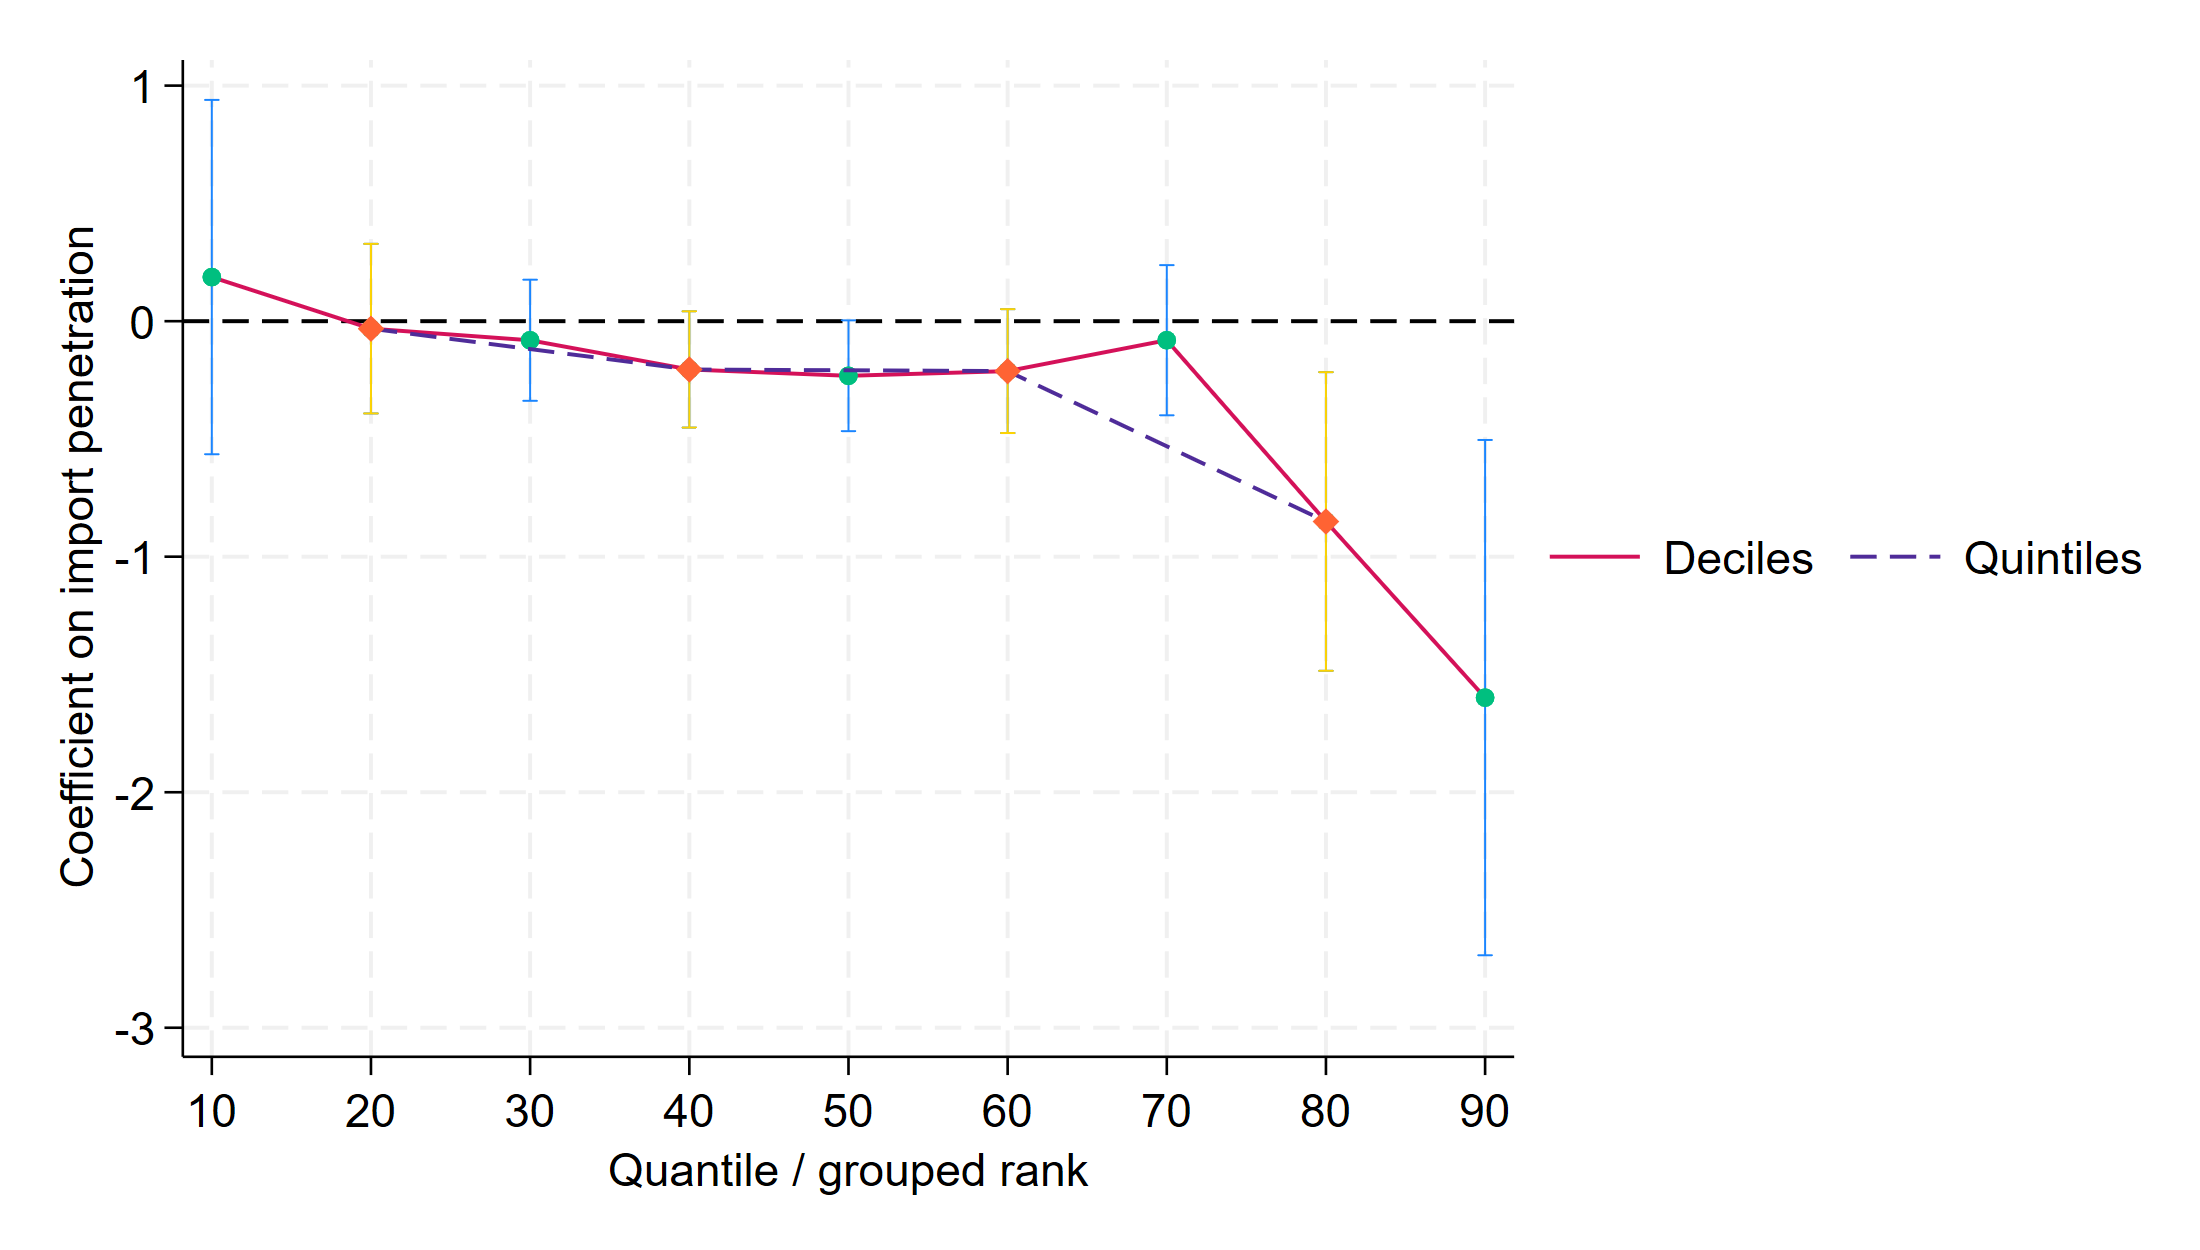
\includegraphics[width=0.85\textwidth]{rob41_decquin_notitle.png}
    \begin{minipage}{0.85\textwidth}
    \footnotesize
    \textit{Notes:} The figure compares the baseline decile estimates with a coarser quintile construction. Points report IV estimates; vertical bars report 95\% confidence intervals. Using quintiles preserves the main shape of the response: estimates remain small through the lower and middle parts of the distribution and become more negative toward the upper tail.
    \end{minipage}
    \caption{Grouped-IV quantile robustness: deciles versus quintiles}
    \label{fig:rob41_decquin}
\end{figure}

\begin{figure}[htbp]
    \centering
    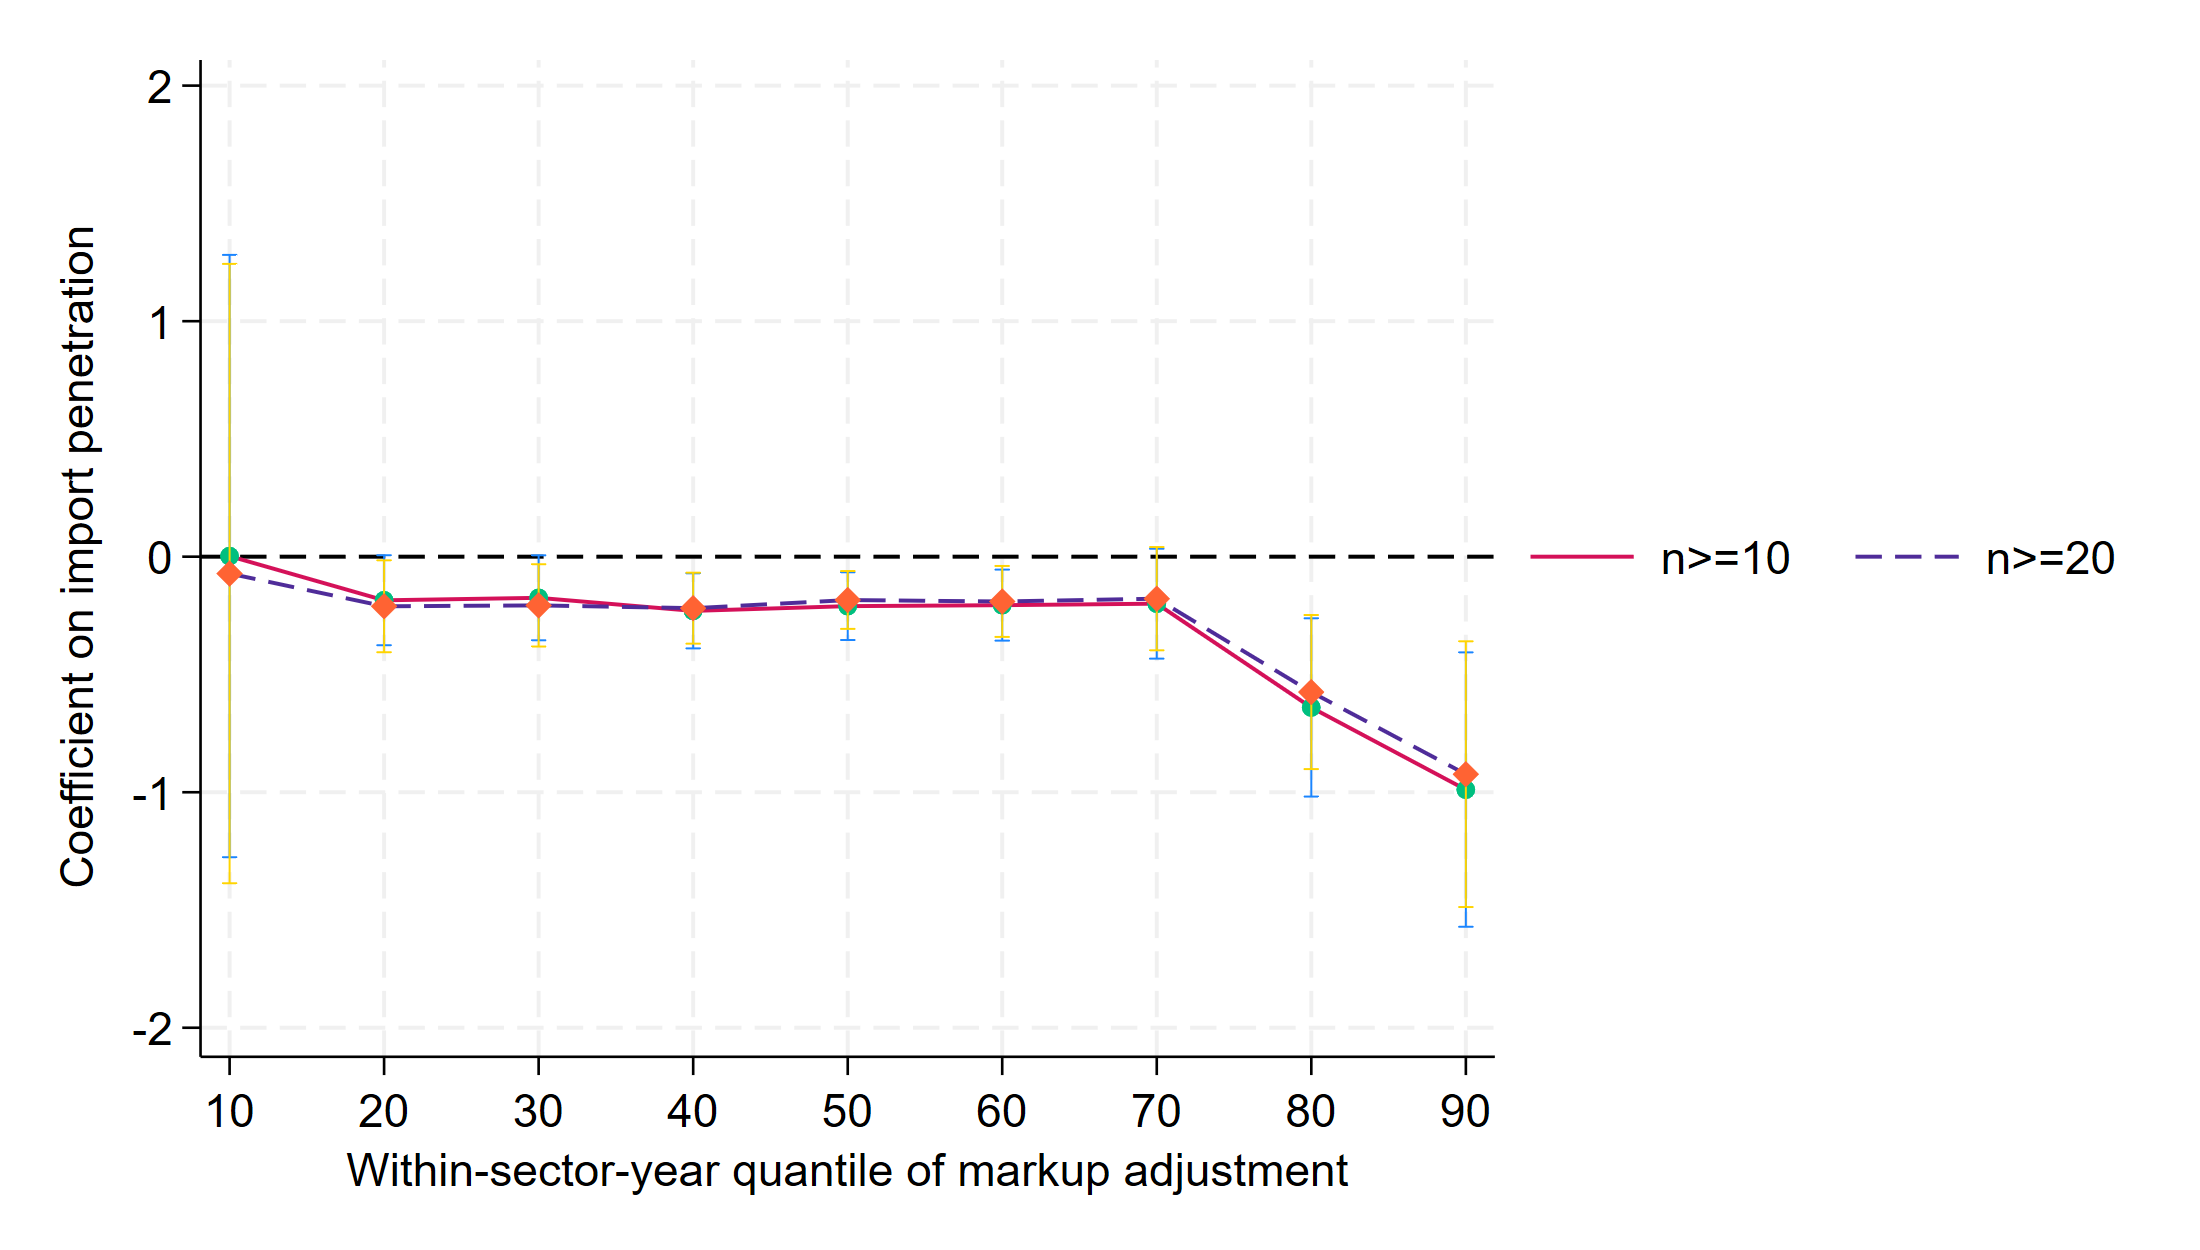
\includegraphics[width=0.85\textwidth]{rob43_thin_notitle.png}
    \begin{minipage}{0.85\textwidth}
    \footnotesize
    \textit{Notes:} The figure excludes thin sector-year cells where empirical quantiles are most sensitive to small-sample order-statistic noise. Points report IV estimates; vertical bars report 95\% confidence intervals. The upper-tail pattern remains visible after this restriction, suggesting that the baseline quantile profile is not driven by a few small cells.
    \end{minipage}
    \caption{Grouped-IV quantile robustness: excluding thin cells}
    \label{fig:rob43_thin}
\end{figure}

The next tables report the finite-sample diagnostics behind the selection diagnostic and grouped-IV quantile correction. The first table uses simulated firm panels with endogenous observation. The second and third tables use simulated sector-year cells to show how the grouped-quantile correction behaves when cell size is correlated with instrument variation.

\begin{table}[htbp]
\centering
\caption{Monte Carlo diagnostic for the selection control function}
\label{tab:mc_selection}
\small
\setlength{\tabcolsep}{5pt}
\begin{fittabular}{llrrrrr}
\toprule
True effect & Specification & Mean beta & Bias & Mean SE & Coverage & Rejection rate \\
\midrule
$\beta_0=0$ & Cubic polynomial & -0.0001 & -0.0001 & 0.0118 & 0.946 & 0.054 \\
& Fifth-order polynomial & -0.0001 & -0.0001 & 0.0118 & 0.946 & 0.054 \\
& Spline, 6 bases & -0.0001 & -0.0001 & 0.0118 & 0.948 & 0.052 \\
& Uncorrected & 0.1134 & 0.1134 & 0.0133 & 0.000 & 1.000 \\
\addlinespace
$\beta_0=0.5$ & Cubic polynomial & 0.4999 & -0.0001 & 0.0118 & 0.946 & 1.000 \\
& Fifth-order polynomial & 0.4999 & -0.0001 & 0.0118 & 0.946 & 1.000 \\
& Spline, 6 bases & 0.4999 & -0.0001 & 0.0118 & 0.948 & 1.000 \\
& Uncorrected & 0.6134 & 0.1134 & 0.0133 & 0.000 & 1.000 \\
\bottomrule
\end{fittabular}
\begin{minipage}{0.88\textwidth}
\footnotesize
\vspace{0.5em}
\emph{Notes:} The table reports Monte Carlo results for the firm-level selection control function with $\theta=0.5$. Coverage is the share of 95 percent confidence intervals containing the true coefficient. For $\beta_0=0$, the rejection rate is the rejection rate of the zero null. For $\beta_0=0.5$, it is the rejection rate against zero. Each design uses 1,000 replications. The average selection rate is approximately 0.491.
\end{minipage}
\end{table}

\begin{table}[htbp]
\centering
\caption{Monte Carlo diagnostic for grouped-IV quantile order-statistic bias}
\label{tab:mc_order_stat}
\scriptsize
\setlength{\tabcolsep}{4pt}
\begin{fittabular}{rrrrrrr}
\toprule
& \multicolumn{2}{c}{Mean coefficient} & \multicolumn{2}{c}{Coverage} & \multicolumn{2}{c}{5\% rejection rate} \\
\cmidrule(lr){2-3}\cmidrule(lr){4-5}\cmidrule(lr){6-7}
Quantile & Uncorrected & Corrected & Uncorrected & Corrected & Uncorrected & Corrected \\
\midrule
10 & 0.0104 & 0.0126 & 0.666 & 0.770 & 0.334 & 0.230 \\
20 & 0.0070 & 0.0063 & 0.756 & 0.880 & 0.244 & 0.120 \\
30 & 0.0061 & 0.0055 & 0.758 & 0.888 & 0.242 & 0.112 \\
40 & 0.0057 & 0.0045 & 0.796 & 0.902 & 0.204 & 0.098 \\
50 & 0.0060 & 0.0031 & 0.768 & 0.920 & 0.232 & 0.080 \\
60 & 0.0062 & 0.0043 & 0.752 & 0.904 & 0.248 & 0.096 \\
70 & 0.0070 & 0.0050 & 0.702 & 0.886 & 0.298 & 0.114 \\
80 & 0.0092 & 0.0053 & 0.564 & 0.888 & 0.436 & 0.112 \\
90 & 0.0148 & 0.0082 & 0.306 & 0.848 & 0.694 & 0.152 \\
\bottomrule
\end{fittabular}
\begin{minipage}{0.88\textwidth}
\footnotesize
\vspace{0.5em}
\emph{Notes:} The table reports a null Monte Carlo with true grouped-IV quantile effects equal to zero. The corrected specification includes a cubic polynomial in sector-year cell size. Coverage is the share of 95 percent confidence intervals containing zero. Rejection is the share of tests rejecting the zero null at the 5 percent level. The simulation uses 500 replications.
\end{minipage}
\end{table}

\begin{table}[htbp]
\centering
\caption{Upper-tail spline-bootstrap robustness for grouped-IV quantiles}
\label{tab:mc_upper_tail_spline}
\small
\begin{fittabular}{lrrrr}
\toprule
Method & Quantile & Mean beta, corrected & Rejection, uncorrected & Rejection, corrected \\
\midrule
Polynomial control & 80 & 0.0058 & 0.436 & 0.120 \\
Polynomial control & 90 & 0.0089 & 0.692 & 0.165 \\
Spline + bootstrap & 80 & 0.0031 & 0.450 & 0.000 \\
Spline + bootstrap & 90 & 0.0025 & 0.750 & 0.050 \\
\bottomrule
\end{fittabular}
\begin{minipage}{0.88\textwidth}
\footnotesize
\vspace{0.5em}
\emph{Notes:} The table reports a targeted upper-tail null Monte Carlo. The spline-bootstrap correction uses a six-basis spline in sector-year cell size with bootstrap inference. Because the procedure is computationally costly, it is implemented only for Q80 and Q90.
\end{minipage}
\end{table}



\FloatBarrier
\normalsize
\renewcommand{\arraystretch}{1}
\subsubsection{Chinese product concentration}

The next appendix tables ask whether the results are driven by product-level concentration inside Chinese imports rather than by broad import competition. Because firm-level Chinese exporter data are unavailable, I proxy this channel with an HS6 product HHI: within each ISIC4-year, I compute how concentrated Chinese import value is across mapped HS6 products. The preferred specifications use the lagged product HHI as a predetermined control or interaction term.

\begin{table}[htbp]\centering
\def\sym#1{\ifmmode^{#1}\else\(^{#1}\)\fi}
\caption{Chinese Product Concentration and Incumbent Markup Adjustment}
\label{tab:rob_chn_gran_mean}
\small
\setlength{\tabcolsep}{4pt}
\renewcommand{\arraystretch}{1.08}

\begin{fittabular}{L{0.38\textwidth}ccc}
\toprule
& \multicolumn{3}{c}{\textbf{Dependent variable: markup adjustment}} \\
\cmidrule(lr){2-4}
& \textbf{Baseline}
& \makecell{\textbf{Add Chinese}\\\textbf{product HHI}}
& \makecell{\textbf{Product HHI}\\\textbf{interaction}} \\
\midrule

\multicolumn{4}{l}{\textbf{Panel A: IV coefficients}} \\

Chinese import-penetration growth
& -0.463\sym{**}
& -0.464\sym{**}
& -0.549\sym{***} \\
& (0.226)
& (0.228)
& (0.197) \\

China IP $\times$ Chinese product HHI
& 
& 
& -0.383 \\
& 
& 
& (0.265) \\

Lagged Chinese product HHI
& 
& -0.001
& -0.002 \\
& 
& (0.003)
& (0.003) \\

Chinese input-supply exposure
& 0.531
& 0.526
& 0.481 \\
& (0.477)
& (0.480)
& (0.467) \\

\midrule
\multicolumn{4}{l}{\textbf{Panel B: Implied import-penetration effect}} \\

At Chinese product HHI $-1$ s.d.
& 
& 
& -0.166 \\

At Chinese product HHI mean
& -0.463
& -0.464
& -0.549 \\

At Chinese product HHI $+1$ s.d.
& 
& 
& -0.932 \\

\midrule
Observations
& 30,269
& 30,269
& 30,269 \\

F-stat
& 24.79
& 24.07
& 12.78 \\

Sector FE
& Yes & Yes & Yes \\

Year FE
& Yes & Yes & Yes \\

Lagged firm controls
& Yes & Yes & Yes \\

\bottomrule
\end{fittabular}

\begin{minipage}{0.92\textwidth}
\footnotesize
\emph{Notes:} The table tests whether concentration of Chinese imports across HS6 products explains the baseline markup-discipline result. Chinese product HHI is computed within ISIC4-year cells using Chinese import values across mapped HS6 products and is standardized in the baseline estimation sample. Chinese import penetration and the interaction term are instrumented by the corresponding output-IV terms. All specifications include ISIC4 sector fixed effects, year fixed effects, lagged firm controls, the Chinese input-supply exposure control, and pre-period labor-share $\times$ post-2016 controls. Standard errors are clustered by ISIC4 sector. 
\sym{*} \(p<0.10\), \sym{**} \(p<0.05\), \sym{***} \(p<0.01\).
\end{minipage}
\end{table}

\FloatBarrier

Table~\ref{tab:rob_chn_gran_mean} adds this product-concentration measure to the mean IV specification. The import-penetration coefficient remains negative and close to the baseline; the interaction terms are imprecise. The diagnostic therefore does not support the view that the main markup response is mechanically driven by a few granular Chinese products.

\begin{table}[htbp]\centering
\def\sym#1{\ifmmode^{#1}\else\(^{#1}\)\fi}
\caption{Grouped IV quantiles: Chinese product concentration interaction}
\label{tab:rob_chn_gran_givq_foreign}
\small
\setlength{\tabcolsep}{4pt}
\renewcommand{\arraystretch}{1.08}
\begin{fittabular}{L{0.42\textwidth}*{4}{c}}
\toprule
                &\multicolumn{1}{c}{(1)}&\multicolumn{1}{c}{(2)}&\multicolumn{1}{c}{(3)}&\multicolumn{1}{c}{(4)}\\
                &\multicolumn{1}{c}{Q25}&\multicolumn{1}{c}{Q50}&\multicolumn{1}{c}{Q75}&\multicolumn{1}{c}{Q90}\\
\midrule
Chinese import-penetration growth&  -0.0467         &   -0.200         &   -0.133         &   -1.363\sym{**} \\
                &  (0.202)         &  (0.160)         &  (0.258)         &  (0.523)         \\
China IP $\times$ Chinese product HHI&  0.00505         &  -0.0276         &  -0.0727         &   -0.260         \\
                & (0.0770)         & (0.0673)         &  (0.116)         &  (0.229)         \\
Lagged Chinese product HHI, standardized& 0.000861         &  0.00187         & -0.00454         & 0.000307         \\
                &(0.00341)         &(0.00320)         &(0.00590)         &(0.00660)         \\
Chinese input-supply exposure&   -0.203         &    0.290         &    1.397         &    1.319         \\
                &  (0.655)         &  (0.438)         &  (1.427)         &  (2.088)         \\
\midrule
Sector-year observations&      596         &      596         &      596         &      596         \\
Kleibergen-Paap rk Wald F&     8.24         &     8.24         &     8.24         &     8.24         \\
\bottomrule
\end{fittabular}
\begin{minipage}{0.92\textwidth}
\footnotesize
\emph{Notes:} The dependent variable is the indicated sector-year quantile of firm-level markup growth. Product HHI is the concentration of Chinese import value across mapped HS6 products within an ISIC4-year cell. All specifications include ISIC4 sector fixed effects, year fixed effects, sector-year cell-size polynomial controls, averaged lagged firm controls, the input-supply exposure control, and pre-period size $\times$ post-2016 controls. Chinese import penetration and its interaction with product HHI are instrumented by the corresponding output-IV terms. Standard errors are clustered by ISIC4 sector.
\end{minipage}
\end{table}

\FloatBarrier

Table~\ref{tab:rob_chn_gran_givq_foreign} repeats the check in the grouped-IV quantile design. The upper-tail coefficient remains negative after adding the Chinese product-HHI interaction, while the interaction itself is not precisely estimated.

Overall, these tables are best read as robustness diagnostics. They show that the baseline and upper-tail results are not absorbed by measured concentration of Chinese imports across HS6 products.

\normalsize
\renewcommand{\arraystretch}{1}
\subsubsection{Synthetic control counterfactuals}

I implement a synthetic-control exercise for the highly exposed sector ISIC4 2790, with the outcome being the sector inverse markup (Figures \ref{fig:scm_gap_spec1}--\ref{fig:scm_gap_spec2}). Following Abadie (2021), the method constructs a weighted combination of lower-exposure sectors that closely tracks ISIC4 2790 before the treatment year, then compares the post-treatment path of the treated sector to this synthetic counterfactual. Using the year 2016 as treatment date, the treated sector displays a post-treatment deviation consistent with lower markup growth relative to its synthetic control. The gap is largest shortly after the China shock and narrows toward the end of the sample, suggesting that the markup response is strongest in the short run and partly absorbed over time through firm adjustment, reallocation, or selective survival.

\begin{figure}[htbp]
    \centering
    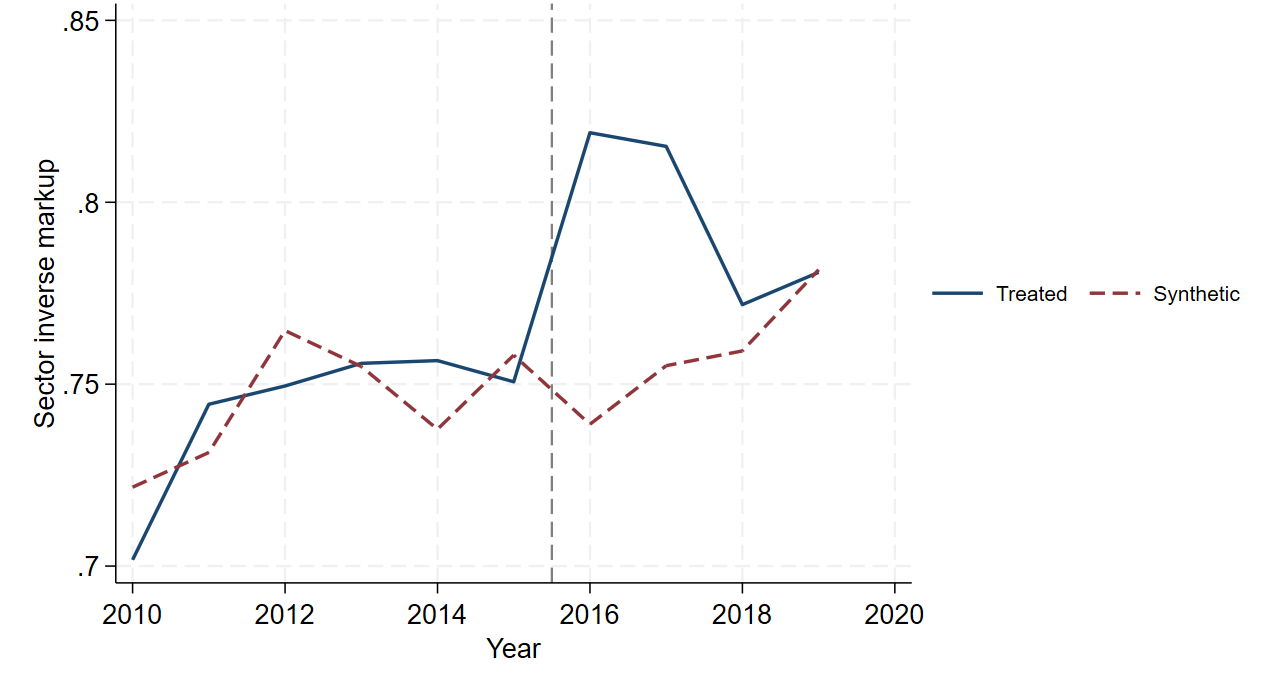
\includegraphics[width=0.82\textwidth]{scm_path_spec2.png}
    \caption{Synthetic-control path: ISIC4 2790, treatment year 2016}
    \label{fig:scm_path_spec2}
\end{figure}

\begin{figure}[htbp]
    \centering
    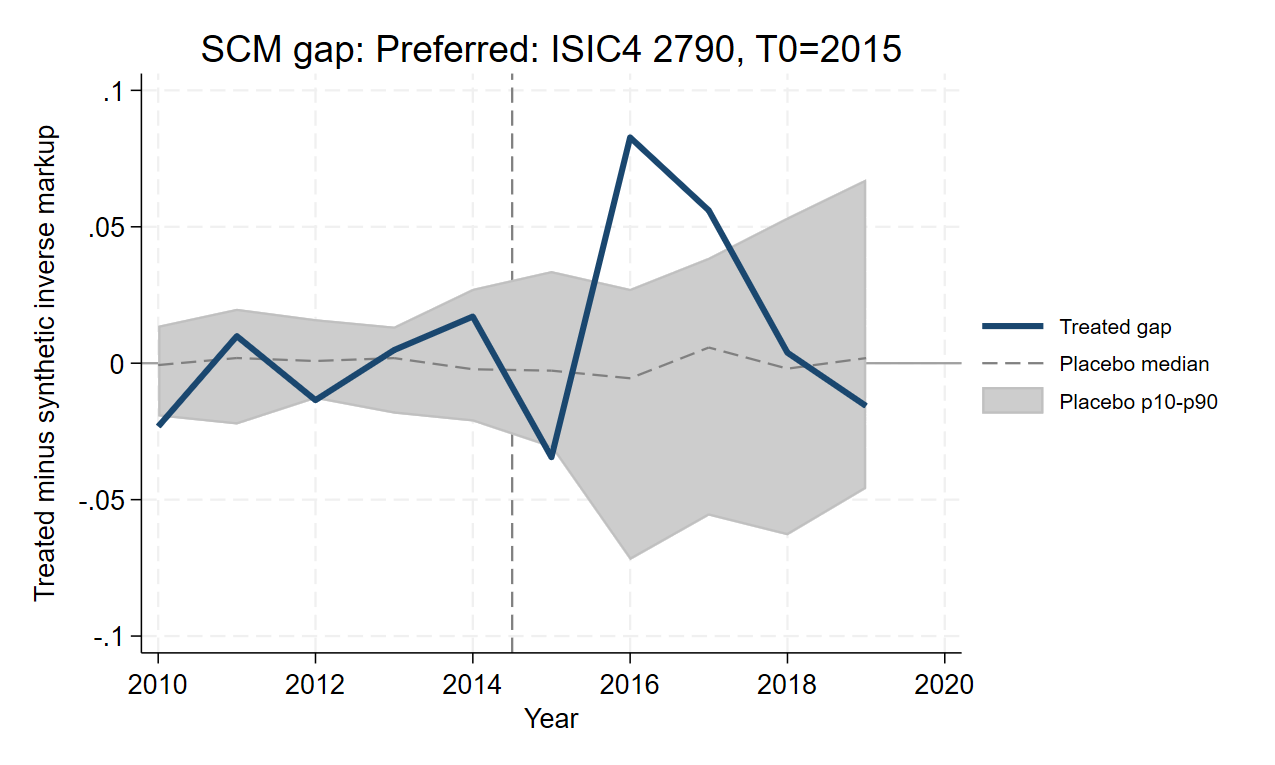
\includegraphics[width=0.82\textwidth]{scm_gap_spec1.png}
    \caption{Synthetic-control gap: ISIC4 2790, treatment year 2016}
    \label{fig:scm_gap_spec1}
\end{figure}

\begin{figure}[htbp]
    \centering
    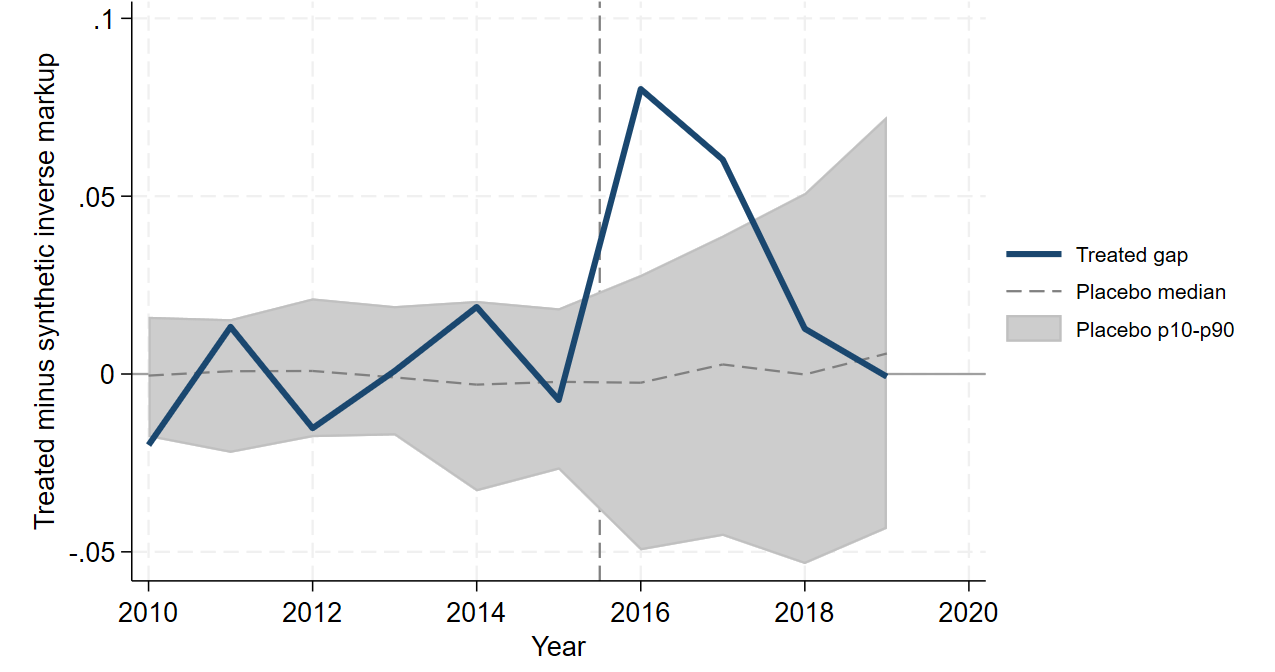
\includegraphics[width=0.82\textwidth]{scm_gap_spec2.png}
    \caption{Synthetic-control gap: ISIC4 2790, treatment year 2016}
    \label{fig:scm_gap_spec2}
\end{figure}



\normalsize
\renewcommand{\arraystretch}{1}
\subsubsection{Internal consistency diagnostics}
\label{app:smm_indirect_inference}

This subsection reports implementation details behind Section~\ref{sec:smm_validation}. The exercise is a restricted SMM check of the output-competition mechanism, not a full structural model of Turkish manufacturing. For each candidate parameter vector \(\theta\), I simulate a panel and compute the same auxiliary IV moments as in the data. The criterion is
\begin{equation}
Q(\theta)=
\left[\widehat m-m^{s}(\theta)\right]'W
\left[\widehat m-m^{s}(\theta)\right],
\end{equation}
where \(\widehat m\) denotes empirical auxiliary moments and \(m^{s}(\theta)\) their simulated counterparts. The targeted moments are the baseline incumbent markup-growth IV coefficient, grouped-IV coefficients at Q80, Q85, and Q90, and the Q90 interaction with sectoral concentration. Sector inverse markups, decomposition terms, input-shock responses, and exit moments are kept as non-targeted diagnostics.

\begin{table}[!htbp]
\centering
\caption{Restricted SMM/calibrated output-competition parameters}
\label{tab:smm_params_app}
\small
\begin{threeparttable}
\begin{fittabular}{L{0.30\textwidth}rL{0.46\textwidth}}
\toprule
Parameter & Value & Interpretation \\
\midrule
\multicolumn{3}{l}{\textit{Estimated output-competition block}} \\
Output scale & 2.138 & Scale of the output-competition channel \\
Output-markup effect & -0.329 & Baseline output-shock effect on markup growth \\
High-markup interaction & -2.102 & Extra output-shock effect for high-markup units \\
Concentration interaction & -2.222 & Extra output-shock effect in concentrated markets \\
Share-dynamics effect & -0.235 & Output-shock component in share dynamics \\
Mean reversion & 1.025 & Auxiliary dynamic-adjustment parameter \\
Drift & 0.350 & Average residual drift in markup dynamics \\
\midrule
\multicolumn{3}{l}{\textit{Externally disciplined parameters and bounds}} \\
\(\eta\) & 1.010 & Across-sector elasticity \parencite{atkesonPricingtoMarketTradeCosts2008} \\
\(\nu\) & 4.000 & Trade elasticity \parencite{simonovskaElasticityTradeEstimates2014} \\
\(\rho\) & 8.000 & Within-sector elasticity \parencite{edmondCompetitionMarkupsGains2015} \\
\(\lambda_{\min}\) & 0.050 & Lower bound for the sectoral exposure/pass-through term \\
\(\lambda_{\max}\) & 0.980 & Upper bound for the sectoral exposure/pass-through term \\
Default \(\lambda\) & 0.850 & Default value used when sector-specific \(\lambda\) is unavailable \\
\bottomrule
\end{fittabular}
\begin{tablenotes}[flushleft]
\footnotesize
\item Notes: The upper panel reports parameters estimated in the restricted SMM exercise. The lower panel reports fixed calibration and bound parameters. Input and selection parameters are fixed at zero, so the exercise summarizes an output-competition block rather than a full model of input pass-through, endogenous exit, or welfare.
\end{tablenotes}
\end{threeparttable}
\end{table}

The signs of the estimated output-competition parameters are consistent with the reduced-form evidence: output competition lowers incumbent markup growth, with stronger effects among high-markup units and in concentrated markets. The remaining elasticity and bound parameters are fixed calibration inputs, not separately estimated from the targeted moments. The mean-reversion coefficient should likewise not be read as a structural persistence estimate; it is an auxiliary adjustment parameter that helps fit the targeted IV moments.

The residual-IV diagnostic also has a narrow interpretation. After subtracting the fitted output-competition component, the residual markup-growth IV coefficient is \(-0.052\) with standard error \(0.295\), using \(31{,}375\) observations, 90 sector clusters, and a first-stage \(F\)-statistic of \(22.93\). Because the fitted component is calibrated to absorb closely related moments, this is an absorption diagnostic rather than an independent holdout validation.

The non-targeted moments show where the restricted block does not travel. The model overstates the sector inverse-markup response relative to the data (\(0.298\) versus \(0.128\)), underpredicts input-shock reallocation (\(2.429\) versus \(8.055\)), and underpredicts the output-shock exit response (\(0.324\) versus \(0.960\)). These gaps are not surprising because the input and selection blocks are switched off. They indicate that input reallocation, endogenous exit, and welfare counterfactuals require a richer structural extension.

The no-output counterfactual is therefore interpreted only as a diagnostic. At the manufacturing level, the average inverse markup changes little, from \(0.5775\) in the fitted path to \(0.5758\) in the no-output path, while the average aggregate markup changes from \(1.7331\) to \(1.7380\). Larger differences appear in specific concentrated sector-years, but they offset in the aggregate. The conclusion is correspondingly local: the fitted mechanism is consistent with incumbent markup discipline in exposed and concentrated markets, not with a full manufacturing-wide welfare effect.



\subsection{Mechanism Evidence and Auxiliary Outcomes}
\label{app:mechanism_appendix}

\subsubsection{Indirect residual-demand evidence}

Lagged-markup interactions (Table~\ref{tab:mech_lagged_interactions}) are statistically meaningful with negative marginal effects at representative distribution points, supporting state dependence.

\begin{table}[htbp]
\centering
\def\sym#1{\ifmmode^{#1}\else\(^{#1}\)\fi}
\caption{Interaction with lagged firm markup}
\label{tab:mech_lagged_interactions}
\begin{threeparttable}
\small
\setlength{\tabcolsep}{5pt}
\renewcommand{\arraystretch}{1.15}
\begin{fittabular}{L{0.40\textwidth}c*{3}{c}}
\toprule
& (1) & \multicolumn{3}{c}{Marginal effect of import competition} \\
\cmidrule(lr){2-2}\cmidrule(lr){3-5}
& $\Delta \log \mu$ & p25 $\mu_{t-1}$ & p50 $\mu_{t-1}$ & p75 $\mu_{t-1}$ \\
\midrule
\multicolumn{5}{l}{\textbf{Panel A: IV coefficients}} \\
Import penetration change ($\Delta IP$) & -1.185\sym{**} & & & \\
& (0.452) & & & \\
$\Delta IP$ $\times$ lagged log markup & 11.52\sym{*} & & & \\
& (6.699) & & & \\
Input-supply shock ($Z^{\text{Input}}$) & 0.265 & & & \\
& (0.592) & & & \\
\addlinespace[0.35em]
\midrule
\multicolumn{5}{l}{\textbf{Panel B: Implied marginal effects}} \\
$\partial \Delta \log \mu / \partial \Delta IP$ & & -2.354 & -1.597 & -0.556 \\
\midrule
Observations & 30551 & & & \\
F-Stat & 9.560 & & & \\
\bottomrule
\end{fittabular}
\begin{tablenotes}[flushleft]
\footnotesize
\item Notes: Standard errors in parentheses. \sym{*} \(p<0.10\), \sym{**} \(p<0.05\), \sym{***} \(p<0.01\).
\end{tablenotes}
\end{threeparttable}
\end{table}

\subsubsection{Input-cost relief and reallocation among continuing firms}

I test input-side mechanisms using sectoral Chinese imported-input dependence $H_j$ and two interaction terms: $Z_{input,jt} \times H_j$ and $\Delta IP_{jt} \times H_j$. The index $H_j = \sum_{k} w_{jk} \bar{s}_k^{\text{CHN}}$ is built from average 2000--2004 Chinese-Turkey input-output weights and China's average import share in upstream Turkish sectors over the same period, so higher values indicate stronger reliance on imported intermediates from China. Table~\ref{tab:input_dep_heterogeneity} shows positive input interaction in markup regression (upstream cost relief) and imprecise output interaction.

\begin{table}[htbp]
\centering
\def\sym#1{\ifmmode^{#1}\else\(^{#1}\)\fi}
\caption{Imported-input dependence heterogeneity}
\label{tab:input_dep_heterogeneity}
\begin{threeparttable}
\small
\setlength{\tabcolsep}{4pt}
\begin{fittabular}{L{0.31\textwidth}*{6}{c}}
\hline\hline
            &\multicolumn{1}{c}{(1)}&\multicolumn{1}{c}{(2)}&\multicolumn{1}{c}{(3)}&\multicolumn{1}{c}{(4)}&\multicolumn{1}{c}{(5)}&\multicolumn{1}{c}{(6)}\\
            &\multicolumn{1}{c}{\theadstack{Markup\\Changes}}&\multicolumn{1}{c}{\theadstack{Markup\\Changes}}&\multicolumn{1}{c}{\theadstack{Revenue\\Changes}}&\multicolumn{1}{c}{\theadstack{Revenue\\Changes}}&\multicolumn{1}{c}{\theadstack{Sales\\Changes}}&\multicolumn{1}{c}{\theadstack{Sales\\Changes}}\\
\hline
Output penetration         &      -0.454\sym{**} &      -1.216\sym{*}  &      -1.632\sym{***}&      -1.974         &      -1.629\sym{**} &      -3.227         \\
                                   &     (0.190)         &     (0.681)         &     (0.535)         &     (2.056)         &     (0.631)         &     (3.209)         \\
[0.3em]
Input supply                 &      -2.041\sym{*}  &       0.285         &       0.996         &       2.651         &      -1.721         &       0.325         \\
                                   &     (1.098)         &     (0.412)         &     (3.526)         &     (1.598)         &     (3.388)         &     (1.977)         \\
[0.3em]
Input supply &       125.8\sym{**} &                     &       87.06         &                     &       124.7         &                     \\
  $\times$ China dependence                                 &     (53.42)         &                     &     (205.2)         &                     &     (159.2)         &                     \\
[0.3em]
Output penetration &                     &       16.84         &                     &       7.252         &                     &       35.52         \\
  $\times$ China dependence                                 &                     &     (11.23)         &                     &     (33.32)         &                     &     (56.91)         \\
[0.3em]
\hline
Observations                       &       30551         &       30551         &       24345         &       24345         &       30551         &       30551         \\
$F$-stat                       &       27.71         &       2.743         &       32.03         &       2.845         &       27.71         &       2.743         \\
\hline\hline
\end{fittabular}
\begin{tablenotes}
\small
\item Notes: Standard errors in parentheses. The output-penetration interaction columns have weak first stages and are interpreted as diagnostics only. \sym{*} \(p<0.10\), \sym{**} \(p<0.05\), \sym{***} \(p<0.01\).
\end{tablenotes}
\end{threeparttable}
\end{table}

Output-competition reallocation toward large incumbents (Table~\ref{tab:mech_share_reallocation}): output-shock interactions not significant; input-shock interactions negative for large-firm/concentration proxies. Input exposure works through reallocation, not by strengthening dominant survivors.

\begin{table}[!htbp]\centering
\def\sym#1{\ifmmode^{#1}\else\(^{#1}\)\fi}
\caption{Market-share reallocation toward large incumbents: output competition and input supply}
\label{tab:mech_share_reallocation}
\setlength{\tabcolsep}{3pt}
\begin{fittabular}{L{0.36\textwidth}*{6}{c}}
\hline\hline
            &\multicolumn{1}{c}{(1)}&\multicolumn{1}{c}{(2)}&\multicolumn{1}{c}{(3)}&\multicolumn{1}{c}{(4)}&\multicolumn{1}{c}{(5)}&\multicolumn{1}{c}{(6)}\\
            &\multicolumn{1}{c}{\theadstack{$\Delta \log$\\$\text{market share}$}}&\multicolumn{1}{c}{\theadstack{$\Delta \log$\\$\text{market share}$}}&\multicolumn{1}{c}{\theadstack{$\Delta \log$\\$\text{market share}$}}&\multicolumn{1}{c}{\theadstack{$\Delta \log$\\$\text{market share}$}}&\multicolumn{1}{c}{\theadstack{$\Delta \log$\\$\text{market share}$}}&\multicolumn{1}{c}{\theadstack{$\Delta \log$\\$\text{market share}$}}\\
\hline
Output shock      &      0.0732         &                     &                     &                     &                     &                     \\
   $\times$ lagged firm size         &    (0.0853)         &                     &                     &                     &                     &                     \\
[0.35em]
Input shock   &                     &      -0.843\sym{*}  &                     &                     &                     &                     \\
  $\times$ lagged firm size          &                     &     (0.451)         &                     &                     &                     &                     \\
[0.35em]
Output shock     &                     &                     &       0.803         &                     &                     &                     \\
  $\times$ large-firm indicator          &                     &                     &     (0.868)         &                     &                     &                     \\
[0.35em]
Input shock  &                     &                     &                     &      -8.689\sym{**} &                     &                     \\
  $\times$ large-firm indicator          &                     &                     &                     &     (3.788)         &                     &                     \\
[0.35em]
Output shock      &                     &                     &                     &                     &       1.787         &                     \\
  $\times$ CR4 membership           &                     &                     &                     &                     &     (1.379)         &                     \\
[0.35em]
Input shock    &                     &                     &                     &                     &                     &      -12.43\sym{**} \\
 $\times$ CR4 membership           &                     &                     &                     &                     &                     &     (6.086)         \\
\hline
Observations&       28159         &       35379         &       28159         &       35379         &       28159         &       35379         \\
F-stat      &       33.40         &                     &       0.904         &                     &       3.238         &                     \\
\hline\hline
\multicolumn{7}{l}{\footnotesize Notes: Standard errors in parentheses. \sym{*} \(p<0.10\), \sym{**} \(p<0.05\), \sym{***} \(p<0.01\)}\\
\end{fittabular}
\end{table}

\subsubsection{Auxiliary outcomes}

Table~\ref{tab:aux_outcomes} applies the mechanism design to revenue, domestic sales, and exports. The import-penetration coefficients are negative for revenue and domestic sales and imprecise for exports. These outcomes support the domestic-demand interpretation of the markup results and help rule out a story driven mainly by export redirection.

\begin{table}[!htbp]\centering
\def\sym#1{\ifmmode^{#1}\else\(^{#1}\)\fi}
\caption{Auxiliary outcomes: revenue, domestic sales, and exports}
\label{tab:aux_outcomes}
\setlength{\tabcolsep}{3pt}
\begin{fittabular}{L{0.30\textwidth}*{8}{c}}
\hline\hline
            &\multicolumn{1}{c}{(1)}&\multicolumn{1}{c}{(2)}&\multicolumn{1}{c}{(3)}&\multicolumn{1}{c}{(4)}&\multicolumn{1}{c}{(5)}&\multicolumn{1}{c}{(6)}&\multicolumn{1}{c}{(7)}&\multicolumn{1}{c}{(8)}\\
            &\multicolumn{1}{c}{$\Delta \log \mu$}&\multicolumn{1}{c}{$\Delta \log \mu$}&\multicolumn{1}{c}{\theadstack{$\Delta \log$\\$\text{Revenue}$}}&\multicolumn{1}{c}{\theadstack{$\Delta \log$\\$\text{Revenue}$}}&\multicolumn{1}{c}{\theadstack{$\Delta \log$\\$\text{Sales}$}}&\multicolumn{1}{c}{\theadstack{$\Delta \log$\\$\text{Sales}$}}&\multicolumn{1}{c}{\theadstack{$\Delta \log$\\$\text{Exports}$}}&\multicolumn{1}{c}{\theadstack{$\Delta \log$\\$\text{Exports}$}}\\
\hline
Import penetration change ($\Delta IP$)   &      -0.540\sym{**} &      -0.979         &      -1.936\sym{***}&      -1.198         &      -1.627\sym{**} &      -1.515         &      -0.416         &      -11.75         \\
            &     (0.231)         &     (0.927)         &     (0.637)         &     (3.075)         &     (0.673)         &     (3.902)         &     (2.625)         &     (17.31)         \\
[0.35em]
Input-supply shock ($Z^{\text{Input}}$)     &      -6.864         &       0.373         &      -25.19\sym{*}  &       2.866\sym{*}  &       1.743         &       0.847         &       53.26         &      -10.10\sym{*}  \\
            &     (5.884)         &     (0.429)         &     (14.52)         &     (1.661)         &     (18.51)         &     (2.009)         &     (35.05)         &     (5.985)         \\
[0.35em]
Input-supply shock $\times$ imported-input dependence   &       28.65         &                     &       107.9\sym{*}  &                     &      -3.609         &                     &      -234.2\sym{*}  &                     \\
            &     (23.00)         &                     &     (57.56)         &                     &     (70.00)         &                     &     (136.7)         &                     \\
[0.35em]
Import penetration $\times$ imported-input dependence  &                     &       1.861         &                     &      -1.554         &                     &      -0.438         &                     &       36.71         \\
            &                     &     (2.849)         &                     &     (9.161)         &                     &     (12.14)         &                     &     (52.04)         \\
\hline
Observations&       30551         &       30551         &       24345         &       24345         &       30551         &       30551         &       19327         &       19327         \\
KP rk Wald $F$&                   &                   &         26.97          &         26.97         &         24.81          &         24.81          &         32.57           &        32.57           \\
\hline\hline
\multicolumn{9}{l}{\footnotesize Notes: Standard errors in parentheses. \sym{*} \(p<0.10\), \sym{**} \(p<0.05\), \sym{***} \(p<0.01\)}\\
\end{fittabular}
\end{table}

\end{document}
